%thesis.tex 
%Model LaTeX file for Ph.D. thesis at the 
%School of Mathematics, University of Edinburgh

%\documentclass[11pt,twoside,openright]{report} 
\documentclass[11pt,oneside]{report} 

%% \titleformat{command}[shape]{format}{label}{sep}{before}[after]

\usepackage{titlesec}
%\usepackage[tracking=true]{microtype}
%\titleformat{\chapter}[display]
%  {\normalfont\huge\bfseries}
%  {\filcenter\underline{\MakeUppercase{\textls[400]{\chaptertitlename}}\ \thechapter}}
%  {20pt}{\Huge}

%\usepackage{epsf}
\usepackage{amsmath}
\usepackage{color}
\usepackage{natbib}
\usepackage{framed}
%\usepackage{cite}
\usepackage{tikz}
\usepackage{tikz-cd}

\RequirePackage{amsmath}
\RequirePackage{amssymb}
\RequirePackage{amsthm}
%\RequirePackage{algorithmic}
%\RequirePackage{algorithm}
%\RequirePackage{theorem}
%\RequirePackage{eucal}
\RequirePackage{color}
\RequirePackage{url}
\RequirePackage{mdwlist}

\RequirePackage[all]{xy}
\CompileMatrices
%\RequirePackage{hyperref}
\RequirePackage{graphicx}
%\RequirePackage[dvips]{geometry}

\usepackage{xcolor}
\usepackage{amsmath,amsfonts,amssymb}
\usepackage{graphicx}
\usepackage[caption=false]{subfig}
\usepackage{enumerate}
\usepackage{mathrsfs}


\titleformat{\chapter}[display]
{\normalfont\Large\filcenter\sffamily}
{\titlerule[1pt]%
\vspace{1pt}%
\titlerule
\vspace{1pc}%
\LARGE\MakeUppercase{\chaptertitlename} \thechapter}
{1pc}
{\titlerule
\vspace{1pc}%
\Huge}
[
%\begin{center}
%%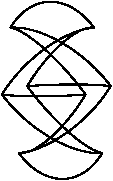
\includegraphics[width=0.8\columnwidth]{pic-deco.pdf}
%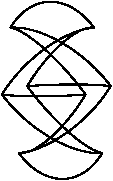
\includegraphics{pic-deco.pdf}
%%\includegraphics{plot-011-tt.pdf}
%\end{center}
%\newpage
]


%\usepackage{epstopdf} % to include .eps graphics files with pdfLaTeX

%\usepackage[pdfpagelabels,pdftex,bookmarks,breaklinks]{hyperref}

\definecolor{darkblue}{RGB}{0,0,127} % choose colors
\definecolor{darkgreen}{RGB}{0,150,0}
%\hypersetup{colorlinks, linkcolor=darkblue, citecolor=darkgreen, filecolor=red, urlcolor=blue}
%\hypersetup{pdfauthor={Simon Burton}}
%\hypersetup{pdftitle={Foo Foo}}

\usepackage[normalem]{ulem}

\usepackage{setspace}   %Allows double spacing with the \doublespacing command

\newcommand{\todo}[1]{\textcolor{red}{#1}}

\newcommand{\Eref}[1]{(\ref{#1})}
\newcommand{\Fref}[1]{Fig.~\ref{#1}}
%\newcommand{\Aref}[1]{Appendix~\ref{#1}}
\newcommand{\SRef}[1]{section~\ref{#1}}


\def\Complex{\mathbb{C}}
\def\C{\mathbb{C}}
\def\R{\mathbb{R}}
\def\Z{\mathbb{Z}}
%\def\Ham{\mathcal{H}} % meh..
\def\Ham{H}
\def\Pauli{\mathcal{P}}
\def\Spec{\mbox{Spec}}
\def\Proveit{{\it (Proof??)}}
\def\GL{\mathrm{GL}}
\def\half{\frac{1}{2}}
\def\Stab{S}


\newcommand{\ket}[1]{|{#1}\rangle}
\newcommand{\expect}[1]{\langle{#1}\rangle}
\newcommand{\bra}[1]{\langle{#1}|}
\newcommand{\ketbra}[2]{\ket{#1}\!\bra{#2}}
\newcommand{\braket}[2]{\langle{#1}|{#2}\rangle}

%\newcommand{\todo}[1]{\textcolor{red}{#1}}

\def\smbox#1{\ \ \mbox{#1}\ \ }



\newcommand{\Field}{\mathcal{F}}
\def\Im{\mathrm{im}}
\def\Ker{\mathrm{ker}}
\def\Dim{\mathrm{dim}}
%\def\euler{\chi}
\def\euler{\mu}


\title{Non-Abelian Quantum Codes}
\author{Simon David Burton}
\date{2016}

\usepackage[phd]{edmaths}
\flushbottom

\begin{document}

\pagenumbering{roman}

\maketitle

%\doublespacing
%\onehalfspacing

\begin{abstract}
Like their classical counterparts,
quantum codes are designed to protect quantum
information from noise.
From the perspective of information theory
one considers the operations required to restore
the encoded information given a syndrome which
diagnoses the noise.
From a more physics perspective, one considers
systems whose energetically protected groundspace
encodes information.
In this work we show that standard error correction
procedures can be applied to systems where the
noise appears as non-abelian Fibonacci anyons.
In the case of a Hamiltonian with non-commuting
terms, we build a theory describing the spectrum of
these models,  
with particular focus on the 3D gauge color code model.
Numerics support the conjecture that this model is gapped,
which one would expect for a self-correcting quantum memory.
\end{abstract}

\declaration

%\dedication{To X Y Z}

\tableofcontents
%\addcontentsline{toc}{chapter}{Contents}
\newpage
\pagenumbering{arabic}

\chapter{Introduction}

%\chapter{A Homological Perspective on Quantum Codes}
%
\def\Complex {C}
\def\tensor{\otimes}
\def\Tensor{\bigotimes}

\def\Stab{\text{\tt Stab}}
\def\Logical{\text{\tt Logical}}
\def\Error{\text{\tt Error}}
\def\Guage{\text{\tt Guage}}

\def\Set{\widetilde{\text{Set}}}
\def\Top{\widetilde{\text{Top}}}
\def\Vec{\widetilde{\text{Vec}}}
\def\Chain{\widetilde{\text{Chain}}}

\def\ker{\text{ker}}
\def\coker{\text{coker}}
\def\im{\text{im}}

%\def\H{\mathcal{H}}
\def\H{H}
\def\S{S}
\def\Z{\mathbb{Z}}

\def\nin{\not\in}

%\begin{abstract}
%We adopt the category of length-3 chain complexes over
%$\Z_2$ as the canonical definition of the category of
%(CSS) stabilizer codes. 
%In this category we show how
%%RG comes from a retract,
%the tensor product gives the generalized hypergraph 
%product~\cite{Tillich09}~\cite{Freedman13}
%and welding~\cite{Michnicki12} comes from a pushout diagram.
%Motivation is provided by showing these constructions
%in more well known categories.
%Finally we show how to generalize the category to
%handle non-CSS codes.
%\end{abstract}

% ----------------------------------------------------------------------------
%

\section{Introduction}

%For the sake of simplicity we consider CSS Codes.

%We first introduce the abstract notion of a chain complex.
%This is the central concern of the study of homological
%algebra. 
%%Next we show how topological spaces give rise to chain
%%complexes.
%Historically, these constructions came from the study
%of invariants of topological spaces, but have since found
%application in areas of algebra (commutative rings, etc.) disjoint from topology.
%%Then we show how to store topological information in a chain complex
%%and then codes are chains
%Classical linear codes and quantum stabilizer codes
%can also be seen as homological objects.
%The intersection of these two areas give topological
%codes (\cite{Dennis01}, \cite{Freedman02}, \cite{Bombin06}).
%But we also find application
%of abstract homological constructs to building codes.

%In defense of arrows
%Physicists tend to ignore domain and range
%Category theory is a kind of type theory, akin to
%dimensional analysis, is group theory  (free groups)
%where any type is composable (product of two values),
%but for example
%tensor products and contractions force one
%to keep track of composability (hense tensor networks;
%arrow diagrams for physicists.)
%Equations become commuting diagrams.
%Dimensionless constants.. what does the type theory
%say of itself?
%Sometimes dimensional analysis gets you to the answer
%even though you don't know what you are doing. It's smart
%enough to do it for you. Similarly with categories, sometimes
%it's enough to just compose arrows together in some obvious
%way.
% Also compare: Heisenberg Vs Schrodinger picture.
% Heisenberg is the arrows (operators) to Schrodinger's elements (states).

% Arrows help us keep track of which matrices we
% can multiply together!

% QIT is infused with ad-hoc methods. The author feels
% that a more abstract viewpoint will help to corral 
% the explosion of these ad-hoc constructions. [ref D.P.]

% ----------------------------------------------------------------
%
%
%
% ----------------------------------------------------------------


\section{Symplectic structure of stabilizer codes}

We work with vector spaces over the field $\mathbb{Z}_2.$

A quantum CSS code is given by two
parity check matrices $\S_z$ and $\S_x.$

Such a code will be called {\it regular}
when the parity checks have full rank.

Given a regular code, we can
a symplectic structure is any
solution to the following (block)
matrix equation:

$$
\left(
\begin{array}{c}
L_z \\
\S_z \\
T_z \\
\end{array}
\right)\left(
\begin{array}{c}
L_x \\
T_x \\
\S_x \\
\end{array}
\right)^\top = I,
$$

where $I$ denotes the appropriate
identity matrix, and the small $T$
is matrix transposition.

In general this is a non-linear
equation because of the presense
of the quadratic term: $T_zT_x^\top=0.$

To construct solutions given
$\S_z$ and $S_x$ we proceed as follows:

{\it (1)} 
Find $L_z$.
The rows of $L_z$ lie in the kernel of $\S_x$,
chosen to be (arbitrary) elements of the cosets
of $\S_z^\top$. Ie. the rows of $L_z$ span $\ker(\S_x)/Im(\S_z^t)$.

{\it (2)}
Find $L_x$.
We first repeat step {\it (1)} on the dual code ($\S_x$ and $\S_z$
swapped) to find $L_x'$.
We look for $L_x$ such that $L_zL_x^\top=I$
knowing that the rows of $L_x$ lie in the
span of $L_x'.$ Ie.  $ L_x = AL_x'$ for some $A$.
Now solve $L_zL_x^\top A^\top = I$ for $A.$

{\it (3)}
Find $T_z$. This will be a solution
of the linear system:

\begin{align*}
    (*)\ \ \S_x T_z^\top &= I \cr
    L_x T_z^\top &= 0.\cr
\end{align*}

The solution space has kernel spanned by
the rows of $\S_z.$

{\it (4)}
$T_z$ is now a solution of the linear system:
\begin{align*}
    \S_z T_x^\top &= I \cr
    L_z T_x^\top &= 0\cr
    T_z T_x^\top &= 0.\cr
\end{align*}

From $(*)$ above, we know that $T_z$ has
full rank, and so this system has a unique
solution $T_x.$




% ----------------------------------------------------------------
%
%  The boundary of the boundary is empty
%
% ----------------------------------------------------------------


\section{The boundary of the boundary is empty}


\subsection{Chain complexes}

We introduce the category of chain complexes, $\Chain$.

A {\it chain complex} $C$ is given by a sequence of vector spaces
${C_i}$ and linear maps $d_i:C_i\to C_{i-1}$ such that $d_{i-1}d_i=0$
for all $i$.

Here is a diagram:

\begin{center}
%\includegraphics[width=0.5\textwidth]{mypicture.png}
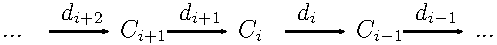
\includegraphics{chain.pdf}
\end{center}

The condition $d_{i-1}d_i=0$ is equivelant to
%requiring $\text{image}(d_i) \subseteq \text{kernel}(d_{i-1})$.
requiring the image of $d_i$ to be contained within the kernel of $d_{i-1}$:

\begin{center}
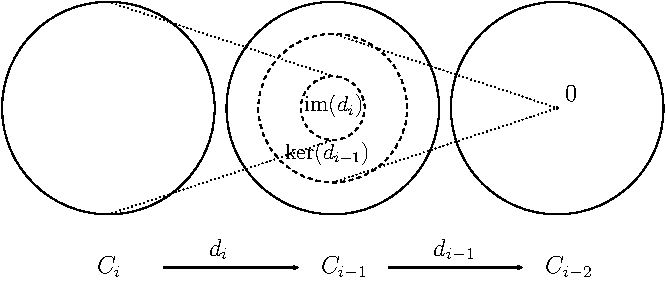
\includegraphics{figure_02.pdf}
\end{center}

Elements of the space $ B_i := \im(d_{i+1}) $ are known as {\it boundaries},
and elements of $ Z_i := \ker(d_i) $ are also known as {\it cycles}.

We form the quotient vector space
$\H_i(C) := B_i(C) / Z_i(C)$,
%$H_i := im(d_{i+1}) / kern(d_i)$,
called the i'th homology 
%vector space.
group (the group operation is given by the vector space addition.)
%We use a different font to dissambiguate the parity
%check matrix, which gets the regular font $H$.

The sequence of spaces ${\H_i}$ will also be denoted as
simply $\H.$ It can be taken to be a chain
complex with the zero boundary map.

We can always consider finite length chain complexes
by appending/prepending zero vector spaces and maps,
for example $A \to B \to C$ can be extended as

    $$ ... \to 0 \to A \to B \to C \to 0 \to ... $$


\subsection{Chain maps}

A chain map $f:C\to C'$ is a sequence of linear maps
$f_i:C_i\to C'_i$ that commute (intertwine) with the boundary map:
$f_{i-1}d_i = d'_if_i.$
Or in diagram form:

\begin{center}
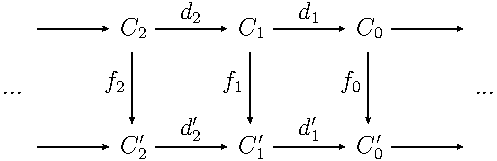
\includegraphics{chainmap.pdf}
\end{center}

The main point about
a chain map is that it
induces a (linear) map of homology groups:

    $$\tilde{f}_i : \H_i\to\H'_i.$$



\subsection{The Hom functor}

%We consider the action of the boundary
%operator by pre-composition:

We consider the boundary operator acting
by pre-composition:

\begin{center}
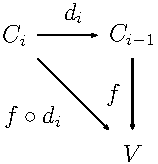
\includegraphics{compose.pdf}
\end{center}

Given a chain complex $C$ and an arbitrary vector
space $V$ we see that the boundary
map $d_i$ acts on maps $f:C_{i-1}\to V$ to give a map $C_i\to V.$
We will fix $V$ to be the underlying field $\Z_2$ then
this action is ``multiplying on the right'',
ie. the transpose operation.
In this way we construct the dual cochain.


\begin{center}
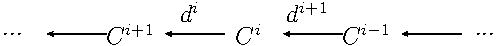
\includegraphics{cochain.pdf}
\end{center}

This is the familiar covector construction.
In general, the so-called hom functor reverses the
direction of all the arrows (of some diagram.)
In our case this means simply that the transpose of a
product reverses the product: $(AB)^\top = B^\top A^\top.$

% ----------------------------------------------------------------
%
%
%
% ----------------------------------------------------------------


% Put this in the intro ??
%
%\subsection{Topologies give chain complexes}
%
%Homology theory in algebraic topology
%
%The boundary of a disc is a circle.
%The boundary of a circle is empty.
%A circle on a sphere is the boundary of a disc,
%but on a torus a circle may not always bound a disc.
%The homology of a space measures the failure of cycles to
%bound a higher dimensional object.
%
%% *** figure here ***
%
%There are many ways to carve up a space such that
%we can perform arithmetic (linear combinations) on
%finite dimensional objects within.
%Definition of n-dimensional object and it's
%(n-1)-dimensional boundary, such that these
%boundaries have trivial boundary themselves.
%
%Cubical (or simplicial) singular homology.
%\cite{Massey}.


\subsection{Classical linear codes}

A classical linear code may be specified as the
kernel of a parity check matrix $\S:\Z_2^n\to \Z_2^m.$
As a chain complex, this is the homology group at
$\Z_2^m.$

As a notational convenience we will sometime denote
a vector space by its (integer) dimension,
eg. $\S:n\to m.$

\setlength{\tabcolsep}{15pt}

\begin{center}
\begin{tabular}{ c c }
\underline{Chain}           &   \underline{Cochain}       \\[8pt]
%$\S:n\to m$      &      $\S^\top:m\to n$    \\[8pt]
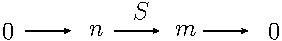
\includegraphics{classchain.pdf}   &  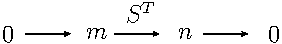
\includegraphics{classcochain.pdf} \\[8pt]
$\H_1=\ker(\S)=:L$  &   $\H^0=\ker(\S^\top) =: L^\top $   \\[8pt]
$\H_0=m/{\im(\S)}=\coker(\S)$ &     $\H^1=n/{\im(\S^\top)}=\coker(\S^\top)$     \\[8pt]
\end{tabular}
\end{center}


\subsection{Quantum stabilizer codes}


A quantum (CSS) code is given by two parity
check matrices $\S_X:n\to m_X$ and $\S_Z:n\to m_Z,$
such that the chain condition $ \S_X \S_Z^\top = 0$
is satisfied.


\begin{center}
\begin{tabular}{ c c }
\underline{Chain}           &   \underline{Cochain}       \\[8pt]
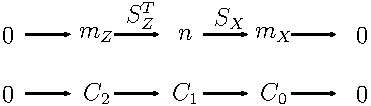
\includegraphics{quchain.pdf}     &  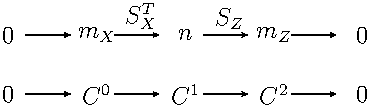
\includegraphics{qucochain.pdf} \\[8pt]
$\H_2=\ker(\S_Z^\top)$                &   $\H^0=\ker(\S_X^\top) $   \\[8pt]
$\H_1=\ker(\S_X)/\im(\S_Z^\top)=:L_X$  &   $\H^1=\ker(\S_Z)/\im(\S_X^\top) =: L_Z $   \\[8pt]
$\H_0=m_X/{\im(\S_X)}=\coker(\S_X)$             &   $\H^2=m_Z/{\im(\S_Z)}=\coker(\S_Z)$     \\[8pt]
\end{tabular}
\end{center}

In the chain we are thinking of the space
$m_Z$ as the space of ``2-dimensional'' objects.
In the toric code this is the space of plaquettes,
but more generally we can think of these as ``generator
labels''. The space $n$ is associated with the physical
qubits, this is where the pauli operators reside.

\begin{center}
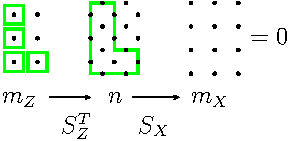
\includegraphics{toric_mZ.pdf}
\end{center}

In the toric code $n$ is the space of ``1-dimensional'' error
operators. The space $m_X$ is then the space of
(X-type) syndrome measurements. In the toric code
these are the ``zero-dimensional'' end-points of (Z-type)
error operators.

\begin{center}
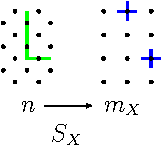
\includegraphics{toric_mX.pdf}
\end{center}


% ----------------------------------------------------------------
%
%
%
% ----------------------------------------------------------------



\section{Tensor product}


The tensor product $C\otimes C'$ of two chain complexes $(C, d)$ and $(C', d')$
is given by

%    $$ (C\otimes C')_i = \bigoplus_{j+k=i} C_j\otimes C'_k $$
    $$ (C\otimes C')_i = \sum_{j+k=i} C_j\otimes C'_k $$

%This is a sum along the diagonals, for example:

with boundary map

    $$ d(c\otimes c') = d(c)\otimes c' + (-1)^{deg(c)}c\otimes d'(c').$$


%We now consider the following two dimensional diagram
%formed from two chain complexes $C$ and $C'$:

%We would like to form a product $C\otimes C'$ of two chain
%complexes $C$ and $C'$. To this end consider the following
%diagram:

To motivate these formulae, consider the following
two dimensional complex:

\begin{center}
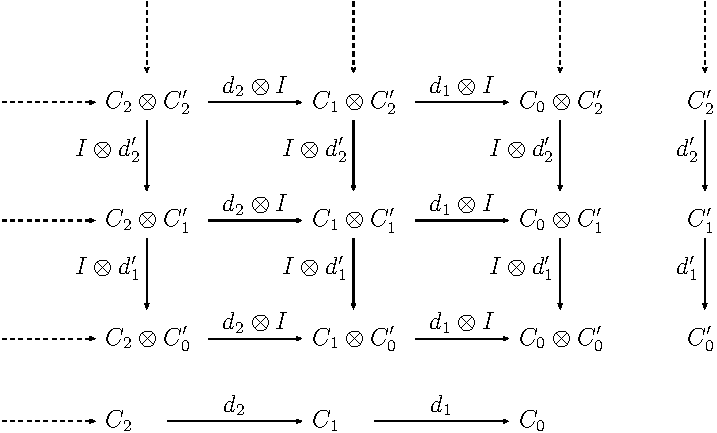
\includegraphics{figure_03.pdf}
\end{center}

where $I$ indicates the appropriate identity map on each vector space.

To reduce this to a one dimensional structure we
(direct) sum along the diagonals, for example:

%Tensor product of two length three chain complexes
\begin{center}
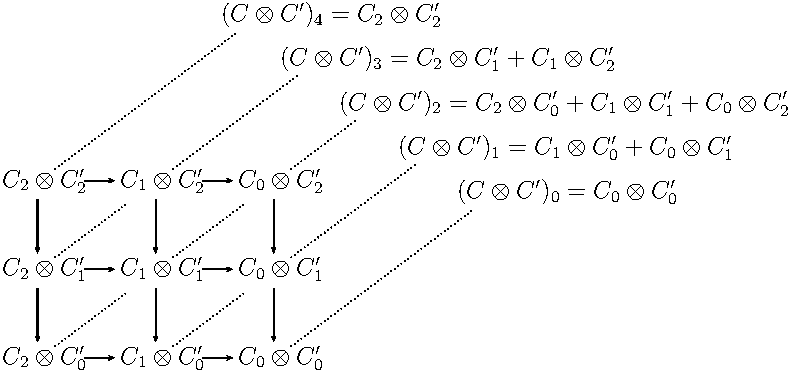
\includegraphics{figure_04.pdf}
\end{center}

Now we add the arrows in an alternating fashion to get a boundary map.
The composition of two arrows in the same direction is
evidently zero, and
we use an alternating weight 
to force the two paths around each square to cancel:

\begin{center}
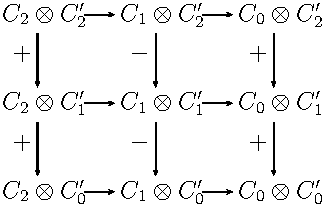
\includegraphics{figure_05.pdf}
\end{center}

With this definition of tensor product the category of
chain complexes becomes a monoidal category 
(See \cite{Baez09}, section 2.3 for a helpful discussion of
monoidal categories.)
%For the categorical definition of the tensor
%product see \cite{Baez09}, section 2.3.

\subsection{The Kunneth formula}

The homology group of the product inherits the same structure
as the underlying chain complex.
This is the import of the Kunneth formula:

    $$ \H_i(C\otimes C') = \sum_{j+k=i} \H_j(C) \otimes \H_k(C') $$

We now define a homomorphism
$ f:\H(C)\otimes \H(C') \to \H(C\otimes C')$
by its action on the subspaces: 
    $$ f:\H_j(C)\otimes \H_k(C') \to \H_{j+k}(C\otimes C').$$

defined by choosing $u_j\in \ker(d_j), u'_k\in \ker(d'_k)$
and then noting that 
    $$ (d_j\otimes I)(u_j\tensor u'_k) = 0,\ \ 
        (I\otimes d'_k)(u_j\tensor u'_k) = 0 $$
which means $u_j\tensor u'_k$ is in the kernel
of the tensor product boundary map, and so represents
an element of $\H_{j+k}(C\otimes C').$
Next check that the choice of $u_i, u'_j$ did not matter...

Weight of stabilizers...
Weight of logops...


\subsection{Product of two classical codes}


The hypergraph product of Tillich and Zemor \cite{Tillich09} is the
product of a classical code and the dual of a classical code.
We didn't define such a product above, but evidently if we
follow the arrows in the same way (or alternativy,
relabel the cochain) it should all work out.

\begin{center}
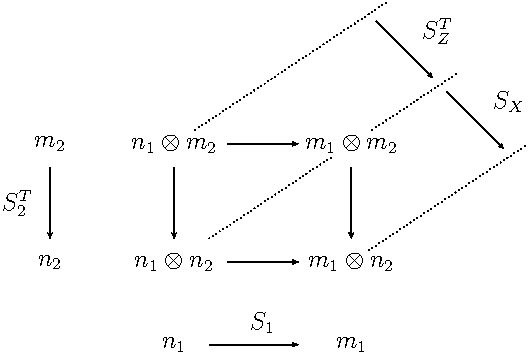
\includegraphics{hyperprod.pdf}
\end{center}

We use the Kunneth formulae to compute the logical
operators:

\begin{align*}
%    \H_1(C_1\otimes C_2^\top)   &= m_1/\im(\S_1)\otimes L_2^\top + L_1 \otimes n_2 / \im(\S_2^\top) \cr
    \H_1(C_1\otimes C_2^\top)   &= \coker(\S_1)\otimes L_2^\top + L_1 \otimes \coker(\S_2^\top) \cr
    |\H_1(C_1\otimes C_2^\top)| &= (m_1-|\im(\S_1)|)|L_2^\top| + |L_1|(n_2 - |\im(\S_2^\top)|) \cr
        &= (m_1-|\im(\S_1^\top)|)|L_2^\top| + |L_1|(n_2 - |\im(\S_2)|) \cr
        &= |\ker(\S_1^\top)||L_2^\top| + |L_1||\ker(\S_2)| \cr
        &= |L_1^\top||L_2^\top| + |L_1||L_2| \cr
\end{align*}

The toric code is obtained from the product of a
(classical) repitition code with its dual.
The important thing to note is that the parity check
matrix (stabilizer generators) is the object of primary
importance, not the space of logical operators.
To get the toric code we must start with a degenerate
parity check matrix  $
\S = \left(
\begin{array}{ccc}
1 & 1 & 0 \\
0 & 1 & 1 \\
1 & 0 & 1 \\
\end{array}
\right).$ 
Then $|L|=|L^\top|=1$ and we get the two logical
qubits in the product.
Using the matrix $
\S = \left(
\begin{array}{ccc}
1 & 1 & 0 \\
0 & 1 & 1 \\
\end{array}
\right).$ gives $|L|=1, |L^\top|=0$ which gives
one logical qubit in the product; this is a surface
code.

\subsection{Product of a classical and a quantum code}

This results in two separate quantum codes, as indicated in
the following diagram:

\begin{center}
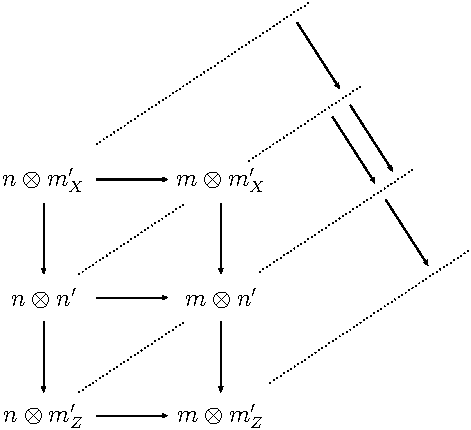
\includegraphics{prodcq.pdf}
\end{center}

(There are also two classical codes at the endpoints.)

In this way we can generate the 3 (spatial) dimension toric code,
as a product of the 2D toric code with the repitition code.
Here we see the two resulting codes have sheets and lines for
logical operators, one code has x-type sheets and z-type lines, the
other code is x-type lines and z-type sheets.

\subsection{Product of two quantum codes}

Continueing this pattern we can generate three different
quantum codes as a product of two quantum codes:

\begin{center}
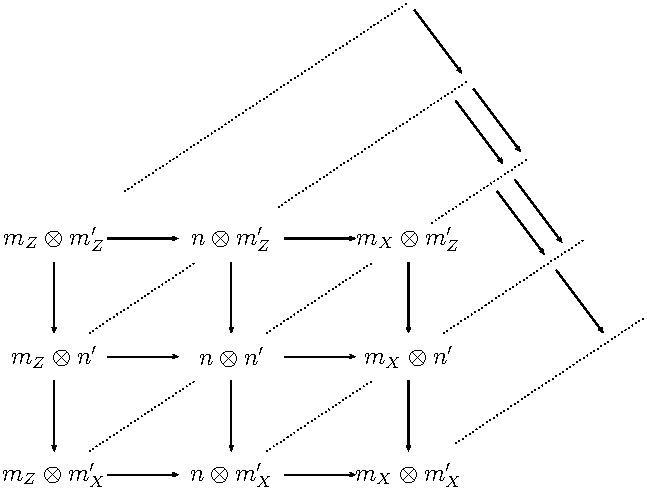
\includegraphics{prodqq.pdf}
\end{center}

For example, the product of the 2D toric code with itself
produces the 4D toric code with x and z type sheet operators,
thats the code in the middle.

Another example, the middle code of the product Stean x Stean has
parameters $[67, 1, 9].$


%\section{Code concatenation}

% ----------------------------------------------------------------
%
%
%
% ----------------------------------------------------------------


\section{Sums and Pushouts}

In any category the sum of two objects $A$ and $B$ is given by
an object $C$ and two maps $f:A\to C$ and $g:B\to C$. These
maps show how to embedd $A$ and $B$ into their ``sum''. A further
requirement is that $C$ is somehow minimal: any other contender
$C'$ for the sum of $A$ and $B$ with ``embedding'' maps $f'$ and $g'$
must factor uniquely through $C$.

In the category of sets we take the disjoint union of $A$ and $B$,
similarly in the category of topological spaces. The embedding
into the sum is the obvious inclusion map.

In the category of vector spaces, we take the direct sum $A\oplus B$, together
with maps $f=I\oplus 0$ and $g=0\oplus I.$
This extends to the category of chain complexes, which 
gives the disjoint union of two codes.

If we would like to join objects $A$ and $B$ along some
``sub-part'', $i:R\to A$, $j:R\to B$ we play the same game
but now require $f$ and $g$ to respect $i$ and $j$, that is,
$f\circ i = g\circ j.$ This is known as a ``pushout'' (of $i$ and $j$.)
In the category of sets, we would take the disjoint union as
before, and then identify those elements according to $(fi)(r) \sim (gj)(r), r\in R.$

This identification also works for topological spaces,
but for vector spaces we project out the {\it subspace} defined
by $fi - gj.$ The notation is then $A\oplus_R B.$

Extended to chain complexes we obtain a general way to
``weld'' two quantum codes together~\cite{Michnicki12}.

TODO...

\section{Non-CSS codes}

TODO...

%\section{Acknowledgements}
%Thanks to Gilles Zemor for some useful hints


%\section{Appendix: stabilizer vs vector space language}



In this chapter we give a brief introduction to
the theory of quantum error correcting codes \cite{Calderbank1997,Dennis2002}.
% focusing on the Kitaev toric code
This will form the foundation for the rest of the thesis,
in terms of being the ``easy'' version of all that follows.

We begin with a consideration of ``size'', or ``counting''.
To count the size of something $A$ we write $\euler(A).$
Size is \emph{additive} in the sense of 
$\euler(A\cup B) = \euler(A) + \euler(B)$ except that
$A$ and $B$ may have intersection.
In this case we would have counted the 
size of the intersection twice and so we modify this formula as
$$
    \euler(A\cup B) = \euler(A) + \euler(B) - \euler(A\cap B).
$$
We can continue this idea to find the
size of the union of three pieces
\begin{center}
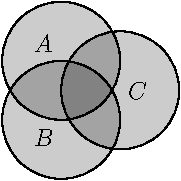
\includegraphics{pic-ABC.pdf}
\end{center}
In this case the formula reads:
\begin{align}\label{EulerAddSub}
\euler(A\cup B\cup C) = \ &\euler(A) + \euler(B) + \euler(C)  \nonumber \\
                     &- \euler(A\cap B) - \euler(A\cap C) - \euler(B\cap C) \nonumber \\
                     &+ \euler(A\cap B \cap C).
\end{align}
The point here is the alternating signs:
each time we try to count a size we overcount by
one intersections worth, subtracting those intersections
goes too far in the opposite direction and so we need
to add intersections of intersections, and so on.

We now wish to apply this idea to count the
size of a sphere. The trick here is to tile the
sphere with the faces of a cube:
\begin{center}
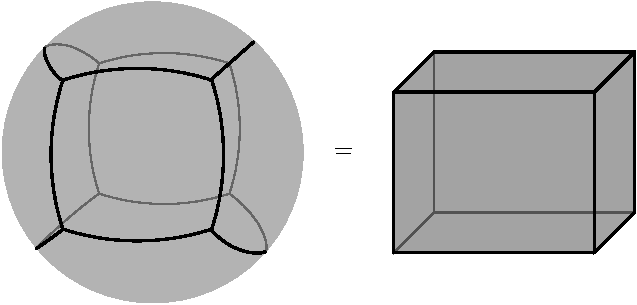
\includegraphics{pic-cube.pdf}
\end{center}
So we have six faces and one might suggest that 
$\euler(S^2)=6$ but these are closed faces, so they
intersect on their edges, of which we have 12.
But these edges intersect at vertices and there are
8 of these. 
We extend the above formula \Eref{EulerAddSub} to calculate:
$$
    \euler(S^2) = 6 - 12 + 8 = 2.
$$
So the sphere has ``size'' two!
The magic here is that any other convex polyhedron would give
the same answer of two.
This, of course, is known as the \emph{Euler characteristic},
and for a sphere this is indeed two.
{This approach to defining Euler characteristic is
discussed in the fascinating book \cite{Klain1997}.}

We repeat this calculation for another surface, a torus.
\begin{center}
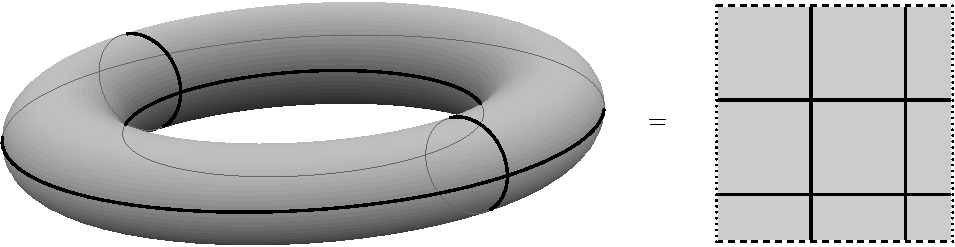
\includegraphics[width=1.0\columnwidth]{pic-torus.pdf}
\end{center}
This time we use four faces, eight edges and four vertices:
$$
    \euler(S^1\times S^1) = 4 - 8 + 4 = 0.
$$

The Euler characteristic has many equivalent definitions,
and we now turn to one of these, which is the idea of a homology.
This theory goes back to Poincar\'e who was trying to
deal with topological issues as they arise in complex analysis~\cite{Lefschetz1970}.
%The first step is to consider vector spaces ...

We are going to replace sets of things by vector
spaces whose basis is the original set.
And just to keep things simple we will 
take our vector spaces over the finite field with
two elements $\Field=\{0, 1\}.$
%That is, we use mod 2 arithmetic when counting things.
This has the distinct advantage
of eliminating all sign errors!

From the set of faces we form a vector space
$C_2$ with basis the set of faces.
Similarly, the one-dimensional pieces are the basis of $C_1$
and the zero-dimensional pieces are the basis of $C_0$:
\begin{align*}
    C_2 &: \mbox{faces},\\
    C_1 &: \mbox{edges},\\
    C_0 &: \mbox{vertices.}
\end{align*}
The formula for Euler characteristic now reads:
\begin{align}\label{EulerEq}
    \euler(C_{\bullet}) = \mbox{dim}(C_2) - \mbox{dim}(C_1) + \mbox{dim}(C_0).
\end{align}
But now things get more interesting,
because we have the following linear operators:
\begin{align}\label{Sequence}
    C_2 \xrightarrow{\ \ \partial_2\ \ } C_1 \xrightarrow{\ \ \partial_1\ \ } C_0.
\end{align}
These are defined to take the ``boundary'' of a shape. 
The operator $\partial_2$ gives the boundary of a face $f\in C_2$
which is just the sum of edges incident to (contained by) that face:
$$
    \partial_2(f) = \sum_{\substack{e\in \text{edges},\\e\sim f}} e.
$$
where we use $\sim$ to indicate incidence, and we extend
$\partial_2$ to all of $C_2$ by linearity.
Similarly, $\partial_1$ is defined to take an edge
to the sum over its vertex endpoints:
$$
    \partial_1(e) = \sum_{\substack{v\in \text{vertices},\\v\sim e}} v.
$$

Now with a small amount of thought one finds that 
$$
    \partial_1 \circ \partial_2 = 0.
$$
This is because each vertex around a face gets counted twice,
and this is zero in $\Field$-linear arithmetic.
\begin{center}
%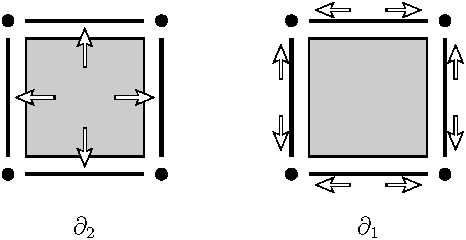
\includegraphics[width=1.0\columnwidth]{pic-bdy.pdf}
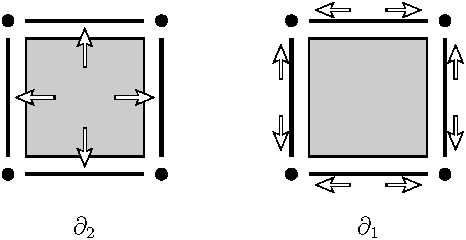
\includegraphics{pic-bdy.pdf}
\end{center}
In other words, the boundary of the boundary is empty!
Or equivalently,
$$
    \Im(\partial_2) \subset \Ker(\partial_1).
$$
%We call the subspace $\Ker(\partial_1)$ the \emph{cycles}
%of $C_1$. 
The subspace $\Ker(\partial_1)$ of $C_1$
will be sums of edges that form closed loops, and we
call these \emph{cycles}.
The subspace $\Im(\partial_2)$ is the space of \emph{boundaries}.
So the above formula
says the space of boundaries is contained within the space of cycles.
This allows us to define the following quotient,
known as the first \emph{homology} group:
$$
    H_1 := \Ker(\partial_1) / \Im(\partial_2).
$$
These are the cycles modulo boundaries.

With a bit more work we can extend the above sequence \Eref{Sequence} to
$$
  0 \xrightarrow{\ \ \partial_3\ \ } 
    C_2 \xrightarrow{\ \ \partial_2\ \ } 
    C_1 \xrightarrow{\ \ \partial_1\ \ } 
    C_0 \xrightarrow{\ \ \partial_0\ \ } 0
$$
so that $\partial_i \circ \partial_{i+1}=0$ 
for $i=0,1,2$
and then define
$$
    H_i := \Ker(\partial_i) / \Im(\partial_{i+1}),\ \ \ \mbox{for}\ \ \ i=0,1,2.
$$

Now we have a new formula for the Euler characteristic,
\begin{align}\label{EulerHom}
    \euler(H_{\bullet}) = \mbox{dim}(H_2) - \mbox{dim}(H_1) + \mbox{dim}(H_0),
\end{align}
which follows from
%from the homology condition
%$\partial_i \circ \partial_{i+1}=0$  and
an application of the rank-nullity theorem to
equation \Eref{EulerEq}.

Going back to the torus example, with four faces,
eight edges and four vertices:
\begin{center}
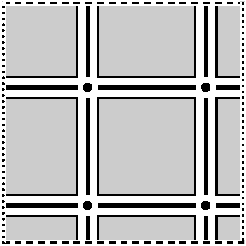
\includegraphics{pic-torus-hom.pdf}
\end{center}
we see that the sum over all faces in $C_2$
has zero boundary,
$$
    \partial_2(\sum_{f\in\text{faces}} f) = 0
$$
and this is the only vector with zero boundary so that
that $\Dim(H_2)=1$.
The space $H_1$ is two dimensional, with representative
cycles given by a vertical or horizontal loop of edges.
Finally, the space $H_0$ is one dimensional: these
are single points.
Putting this together we get
$$
    \euler(S^1\times S^1) = 
    \mbox{dim}(H_2) - \mbox{dim}(H_1) + \mbox{dim}(H_0) = 1-2-1 = 0,
$$
which agrees with our previous calculation for the Euler
characteristic of the torus.

%Because we have $\partial_3=0$ and $\partial_0=0$ this formula
%becomes
%\begin{align}
%    \euler(H_{\bullet}) = \Dim(\Ker{\partial_2}) - \dim(H_1) + \dim(\Im{\partial).
%\end{align}

This is all great but what does it have to do with quantum codes?
Well, before we talk quantum it is worth first going over what we
mean by a code in the classical sense of the word.
We wish to communicate a single bit of information, 
but the communication channel we use suffers from random noise.
This noise acts to randomly toggle bits.
One way to mitigate against this effect is to just
send multiple copies of each bit we wish to communicate.
For example, we send either $000$ or $111$.
Once again it is useful to think of this as a three
dimensional vector over $\Field.$
When the message is recieved any noise can be diagnosed
using the check matrix, $S:\Field^3\to\Field^3:$
$$
S = \left( \begin{array}{lll}
1&1&0\\
0&1&1\\
1&0&1
\end{array} \right).\quad
$$
The codewords belong in the kernel of this operator.
Any failure to be in the kernel is presumed to come
from a noise process.
Notice that this matrix is rank degenerate.
There is a reason for this: we can view it as
the boundary operator for the homology of a circle!
\begin{center}

\includegraphics{pic-circle-hom.pdf}
\end{center}
In this case, there is one bit for each of the three
edges, and the $S$ matrix will record a boundary vertex
between non-identical bits.
$$
  0 \xrightarrow{\ \ \ \ } 
    C_1 \xrightarrow{\ \ S=\partial_1\ \ } 
    C_0 \xrightarrow{\ \ \ \ } 0.
$$

Thinking of the finite field $\Field=\{0,1\}$ as a classical
bit would suggest that the passage to quantum codes involves
taking superpositions over these two bit values.
Indeed this is what we do.
The two dimensional complex Hilbert space that we get
is known as a \emph{qubit}:
$$
    \Complex[\Field] = \{ \alpha \ket{0} + \beta \ket{1}, \ \ \alpha,\beta\in \Complex \}.
$$
Notice how we put the $\Field$-linear values inside the ket.
Taking $n-$fold tensor products
of a qubit corresponds to superpositions over
$n$ dimensional $\Field$-linear values.
This basis we call the \emph{computational basis.}

Using this basis, we write matrices for 
the two important operators, Pauli X and Z:
$$
X = \left( \begin{array}{ll}
0&1\\
1&0\end{array} \right),\quad
Z = \left( \begin{array}{rr}
1&0\\
0&-1\end{array} \right).
$$
These two operators generate the (real) single qubit \emph{Pauli group} $\Pauli_1.$
We call these \emph{bitflip} and \emph{phaseflip} operators, respectively.
For the $n$-qubit Pauli group $\Pauli_n$
we take $n$-fold tensor products of $I, X,$ and $Z,$
where $I$ is the single qubit identity operator.
%Because this is used frequently
We suppress the tensor symbol in such products, for example
writing $XII$ for $X\otimes I\otimes I.$

Now we take the classical repitition code and
try the following quantum version:
$$
    \alpha\ket{0} + \beta\ket{1} \mapsto \alpha\ket{000} + \beta\ket{111}.
$$
To detect any single bitflip error, such as
$XII, IXI$ or $IIX$ 
we measure the \emph{check} operators
$ ZZI, IZZ.$
The outcome of such measurements we call a \emph{syndrome}
because these serve to diagnose an error process.

However, bitflip errors are not the only unitary operators
that we would like to detect.
Indeed, any single bit phaseflip operator, $ZII, IZI$ or $IIZ$
has the effect
$$
    \alpha\ket{000} + \beta\ket{111} \mapsto \alpha\ket{000} - \beta\ket{111}
$$
which goes unnoticed by our syndrome measurements.
Effectively we still have a classical code.

In order to move towards the solution to this problem,
we examine more closely the action of the check operators.
Given any state 
$$
    \ket{\psi} = \alpha\ket{000} + \beta\ket{111}
$$
we have 
$$
    g \ket{\psi} = \ket{\psi}
$$
for $g \in \{III, ZZI, IZZ, ZIZ\}.$
In other words, $\ket{\psi}$ is \emph{stabilized}
by the group generated by $ZZI$ and $IZZ.$
This motivates the following definition.
A \emph{stabilizer code} is 
specified by a commutative subgroup $S$ of $\Pauli_n$
such that $-I\notin S.$
We define the subgroup $\Pauli_n^X$
to be generated by $n$-fold tensor products of the $I$ and $X$ operators.
Similarly, $\Pauli_n^Z$ 
is generated by $n$-fold tensor products of the $I$ and $Z$ operators.

We now make the restriction that the generators of
the stabilizer group come from either $\Pauli_n^X$ or $\Pauli_n^Z$.
This is known as a \emph{CSS stabilizer code}\ \cite{Gottesman1996,Calderbank1997}.

Both of $\Pauli_n^X$ and $\Pauli_n^Z$ are abelian and
isomorphic as groups to the $n$-fold product of $\Z_2$.
But $Z_2$ is more than an abelian group, it's also a field,
which we have been notating as $\Field.$
In this way, we identify these groups with the $n$-dimensional
vector space over the field $\Field:$
$$
\Pauli_n^X \cong \Field^n,\ \ \ 
\Pauli_n^Z \cong \Field^n.
$$
Using this identification, the commutativity of 
operators $u\in\Pauli_n^X$ and $v\in\Pauli_n^Z$
is equivalent to the $\Field$-linear
inner product of $u$ and $v$ being zero.

So the theory of CSS stabilizer codes becomes 
amenable to the theory of finite dimensional vector
spaces. But there's more than this.
It turns out that such a stabilizer code 
is essentially equivalent to a homology!

We show how this works by 
using the above example of torus homology.
Here we separately number
the faces, edges and vertices as
\begin{center}
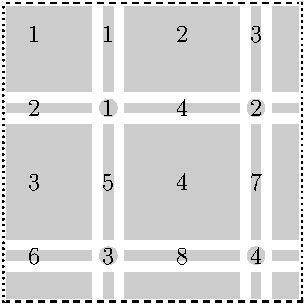
\includegraphics{pic-torus-count.pdf}
\end{center}
Using this ordering 
we write 
the boundary operators as the following matrices, with
zero entries indicated by dots:
\begin{align*}
S_X = \partial_2^{\top} &= \left( \begin{array}{cccccccc}
1&1&1&.&.&1&.&.\\
1&.&1&1&.&.&.&1\\
.&1&.&.&1&1&1&.\\
.&.&.&1&1&.&1&1
\end{array} \right),\\
S_Z = \partial_1 &= \left( \begin{array}{cccccccc}
1&1&.&1&1&.&.&.\\
.&1&1&1&.&.&1&.\\
1&.&.&.&1&1&.&1\\
.&.&1&.&.&1&1&1
\end{array} \right).
\end{align*}

%\begin{align*}
%\partial_2^{\top} &= \left( \begin{array}{cccccccc}
%1&1&1&.&.&1&.&.\\
%1&.&1&1&.&.&.&1\\
%.&1&.&.&1&1&1&.\\
%.&.&.&1&1&.&1&1
%\end{array} \right),\ \ \ \ \ 
%S_X = \left( \begin{array}{c}
%XXXIIXII\\
%XIXXIIIX\\
%IXIIXXXI\\
%IIIXXIXX\\
%\end{array} \right),\\
%\partial_1 &= \left( \begin{array}{cccccccc}
%1&1&.&1&1&.&.&.\\
%.&1&1&1&.&.&1&.\\
%1&.&.&.&1&1&.&1\\
%.&.&1&.&.&1&1&1
%\end{array} \right),\ \ \ \ \ 
%S_Z = \left( \begin{array}{c}
%ZZIZZIII\\
%IZZZIIZI\\
%ZIIIZZIZ\\
%IIZIIZZZ
%\end{array} \right).
%\end{align*}

The rows of $\partial_2^\top$ become the $X$ type generators of
the stabilizer group, and the rows of $\partial_1$ are $Z$ type
generators.
It follows that 
the homology condition $\partial_1\partial_2 = 0$ is
exactly the commutativity requirement $S_Z S_X^\top = 0$ for
a stabilizer code.
Writing $m_X$ for the rows of $S_X$ and $m_Z$ for the rows
of $S_Z$ we have the following sequence:
$$
    \Field^{m_X} \xrightarrow{\ \ S_X^\top\ \ } 
    \Field^{n} \xrightarrow{\ \ S_Z\ \ } 
    \Field^{m_Z}.
$$

The $S_Z$ operators detect bitflip errors $u\in\Field^n$
via $\Field$-linear multiplication on the left:
$$
    v = S_Zu.
$$
This vector is the \emph{syndrome} vector.
We now dissect the space $\Field^n$ according to the kernel of $S_Z$.
Writing $\Field^n$, the space of bitflip operators,
as a direct sum:
$$
    \Field^n = \Ker(S_Z) \oplus T_X
$$
where the kernel of $S_Z$ are the \emph{undetectable errors}, or cycles.
Everything else is in 
the space $T_X,$ which are the \emph{detectable errors}.
The undetectable errors contain the $X$ type stabilizers, or boundaries,
which don't effect the codespace.
Also in the kernel of $S_Z$ are the $X$ type logical operators, which 
we write as $L_X.$
These operators are cycles that are not boundaries, and so they represent
elements of the homology $H_1.$

We already know $S_ZS_X^\top=0$ so that vectors in the row space 
of $S_X$ are undetectable by $S_Z.$
Note that $S_X$ and $S_Z$ are rank degenerate matrices, so
we make the non-degenerate matrices $\tilde{S}_X$ and $\tilde{S}_Z$ 
by deleting rows:
\begin{align*}
\tilde{S}_X = \left( \begin{array}{cccccccc}
1&1&1&.&.&1&.&.\\
1&.&1&1&.&.&.&1\\
.&1&.&.&1&1&1&.
\end{array} \right),\ \ \ 
\tilde{S}_Z = \left( \begin{array}{cccccccc}
1&1&.&1&1&.&.&.\\
.&1&1&1&.&.&1&.\\
1&.&.&.&1&1&.&1
\end{array} \right).
\end{align*}
We find a right inverse to $\tilde{S}_Z$ and form the matrix $T_X$:
$$
    T_X^\top \tilde{S}_Z = I
$$
where $I$ here is the appropriate $F$-linear identity.
This $T_X$ matrix has as rowspace the \emph{detectable errors:}
\begin{align*}
T_X = \left( \begin{array}{cccccccc}
.&.&.&.&1&.&.&1\\
.&.&.&.&.&.&1&.\\
.&.&.&.&.&.&.&1
\end{array} \right).
\end{align*}
The rows of this matrix,
together with those from $\tilde{S}_X$, form a six dimensional
subspace of $\Field^n$.
The other two dimensions are
spanned by operators $L_X$ such that $L_X^\top S_Z=0:$ 
\begin{align*}
L_X = \left( \begin{array}{cccccccc}
1&.&.&.&1&.&.&.\\
.&1&.&1&.&.&.&.
\end{array} \right).
\end{align*}
Together this forms an $(L,S,T)$-decomposition of the CSS
stabilizer code $S$\ \ \cite{Duclos-Cianci2010a,Yoshida2010}.

To see the error correction process more vividly, we expand the
code dimensions.
Here we show a tiling of the torus, with $m_X = 5\times 5$ tiles.
There are two edges per tile, so this code has $n=50$ qubits:
\begin{center}
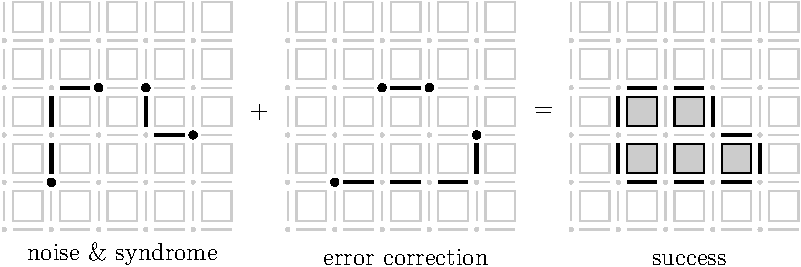
\includegraphics[width=0.8\columnwidth]{pic-toric-suc.pdf}
\end{center}
We show a noise process that acts by bitflip errors
and the resulting syndrome.
The noise process acts on qubits, this is a vector in $\Field^n:$
$$
    c \in \Field^n = C_1.
$$
So the error process is represented as some collection of edges.
The syndrome operator $S_Z$ gives the boundary of these
edges, shown as black vertices.
The error correction procedure takes these boundary vertices
as input and attempts to reconstruct the most likely collection of
edges with this boundary. This then is the operator $c'\in\Field^n$
that is applied to correct the error.
Note that $c+c'$ is a cycle because the vertices of $c$ and $c'$ cancel out.
If the resulting operator $c+c'$ is in the image of $S_X,$
ie. a boundary, then the error correction has succeeded.

Otherwise, $c+c'$ is not a boundary and represents a non-trivial
operator in $H_1$ and will therefore alter the encoded qubits:
\begin{center}
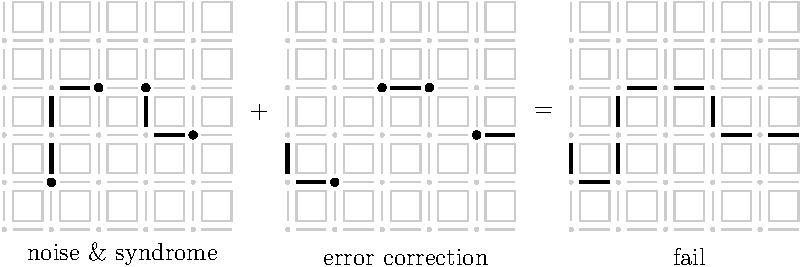
\includegraphics[width=0.8\columnwidth]{pic-toric-fail.pdf}
\end{center}

Given any homology $\partial_1 \partial_2 = 0$
we get another homology by taking the transpose:
$\partial_2^\top \partial_1^\top = 0.$
\begin{center}
%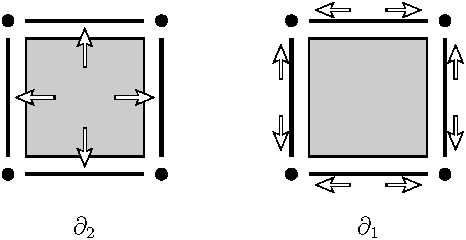
\includegraphics[width=1.0\columnwidth]{pic-bdy.pdf}
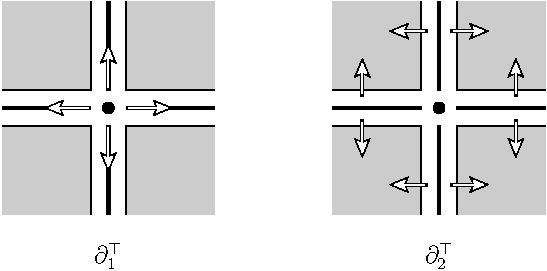
\includegraphics{pic-cobdy.pdf}
\end{center}
In this way we can examine the effect of phase flip errors:
$$
    \Field^{m_Z} \xrightarrow{\ \ S_Z^\top\ \ } 
    \Field^{n} \xrightarrow{\ \ S_X\ \ } 
    \Field^{m_X}.
$$

% ------------------------------------------------------------------

\begin{center}
* \ \ \ \ \ \ \ \ \ \ * \ \ \ \ \ \ \ \ \ \ *
\end{center}

So far we have been considering how to protect quantum information
using the framework of error correction.
An alternative perspective arises by considering energetic
protection.
This works by considering the stabilizer generators $G_0$ as
the terms of a Hamiltonian:
$$
    H = \sum_{g\in G_0} g.
$$
Note that in this thesis we use a neg-Hamiltonian convention,
so that the groundspace belongs to the largest eigenvalue of $H$.
Because all the terms in $H$ commute, we can label the eigenspaces of
this Hamiltonian uniquely by the eigenvalues of the stabilizers.
The groundspace is the simultaneous $+1$ eigenspace of the stabilizers
and therefore corresponds exactly to the stabilized codespace above.

In terms of error correction,
we think of noise processes as being diagnosed by a syndrome. 
But here 
effects of noise are now interpreted energetically, as particle creation.
Any bitflip error ``creates'' particles at the vertex endpoints.
In other words, the syndrome is interpreted as a collection of particles.
These particles are called \emph{anyons}
because of their unusual exchange statistics.

We can write down a basis for the groundspace by summing over
the orbit of the stabilizer code,
$$
    \sum_{g_X\in S_X} g_X \ket{l_X},
$$
where $l_X$ is any logical bitflip operator, written as a computational
basis element (inside the ket).
Such a basis element looks like a so-called string-net condensate:
\begin{center}
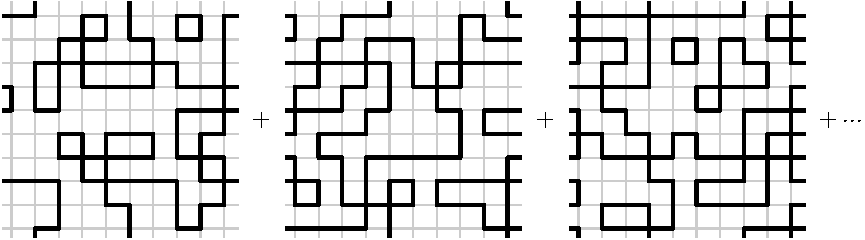
\includegraphics[width=0.8\columnwidth]{pic-toric-liquid.pdf}
\end{center}
It is clear from this picture that the state is stabilized and
hense belongs in the groundspace of $H:$ 
the $S_Z$ stabilizers act as $+1$ on this state because there
are no vertex endpoints, and the $S_X$ stabilizers act to permute
the terms of the sum.

% ------------------------------------------------------------------

\begin{center}
* \ \ \ \ \ \ \ \ \ \ * \ \ \ \ \ \ \ \ \ \ *
\end{center}

There are two approaches to non-abelian codes
explored in this thesis.
The first involves relaxing the commutativity
of the Hamiltonian terms.
These are the gauge code Hamiltonians discussed in chapter 2.
While these Hamiltonians are no longer easily diagonalizable,
we still find the stabilizers playing an important role.
In particular, we generalize the $(L,S,T)$-decomposition to these
Hamiltonians, and show how this relates to the string-net condensation picture.
Building states by summing over the orbit of the terms of the
Hamiltonian is the basic idea behind group representation theory.

With commuting Hamiltonian terms it is easy to find the spectral gap,
which is the difference between the groundspace eigenvalue and the
first excited eigenvalue.
In chapter 2 
we make progress understanding the spectrum of
the non-commuting gauge code Hamiltonians, 
with particular attention payed
to the gap.

The second approach to non-abelian codes can be understood 
from an algebraic topology perspective. 
A practitioner of these arts would likely describe
the fundamental group of a topological space as being the non-abelian 
version of its homology.
And this is indeed closely related to 
the theory of anyons and modular
functors which we describe in chapter 3.
Then in chapter 4, we go on to show how
error correction can be simulated in these systems.

In the abelian theory the following two
processes are equivalent (homologous), but for
general anyon theories this is not the case:
\begin{center}
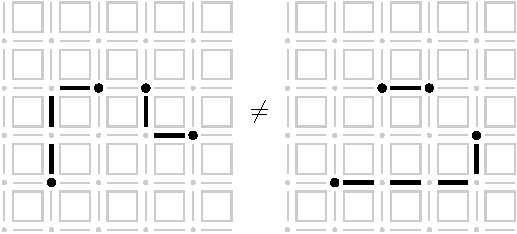
\includegraphics[width=0.5\columnwidth]{pic-toric-nonab.pdf}
\end{center}

While chapter 4 relies on chapter 3, capter 2 is independant of these.

\begin{center}
* \ \ \ \ \ \ \ \ \ \ * \ \ \ \ \ \ \ \ \ \ *
\end{center}

\begin{samepage}
It seems that physics has a long history of surprising encounters
with advanced mathematical concepts,
long after the mathematicians
themselves have finished being excited by them.
This would suggest the following algorithm for
success in theoretical physics:
\begin{enumerate}
\item look at what mathematicians were getting excited about several decades ago,
\item ???
\item profit!
\end{enumerate}
\end{samepage}
This is somewhat the philosophy of the present thesis.
The downfall of this is perhaps that some concepts are
elucidated in an overly technical manner. However, the
author feels this approach to be useful as it makes contact
with a shared mathematical language.

\chapter{Representations and Spectra of Gauge Code Hamiltonians}


%\renewenvironment{framed}[1][\hsize]{%
%\def\FrameCommand{{\color{black}\vrule width 3pt}\hspace{0pt}\fboxsep=\FrameSep\colorbox{lightgray}}%
%\MakeFramed{\hsize0.8\linewidth\advance\hsize-\width\FrameRestore}}
%{\endMakeFramed}

\renewenvironment{framed}
{\begin{samepage}
\MakeFramed{\hsize0.8\linewidth\advance\hsize-\width\FrameRestore}}
{\endMakeFramed\end{samepage}}

%\renewenvironment{framed}
%{\MakeFramed}
%{\endMakeFramed}


\def\Complex{\mathbb{C}}
\def\C{\mathbb{C}}
\def\R{\mathbb{R}}
\def\Z{\mathbb{Z}}
%\def\Ham{\mathcal{H}} % meh..
\def\Ham{H} 
\def\Pauli{\mathcal{P}}
\def\Spec{\mbox{Spec}}
\def\Proveit{{\it (Proof??)}}
\def\GL{\mathrm{GL}}
\def\half{\frac{1}{2}}
\def\Stab{S}

\newcommand{\ket}[1]{|{#1}\rangle}
\newcommand{\expect}[1]{\langle{#1}\rangle}
\newcommand{\bra}[1]{\langle{#1}|}
\newcommand{\ketbra}[2]{\ket{#1}\!\bra{#2}}
\newcommand{\braket}[2]{\langle{#1}|{#2}\rangle}

%\newcommand{\todo}[1]{\textcolor{red}{#1}}

\def\smbox#1{\ \ \mbox{#1}\ \ }

%%%%%%%%%%%%%%%%%%%%%%%%%%%%%%%%%%%%%%%%%%%%%%%%%%%%%%%%%%%%%%%%%%%%%%%%%%%%%%%
%
%%%%%%%%%%%%%%%%%%%%%%%%%%%%%%%%%%%%%%%%%%%%%%%%%%%%%%%%%%%%%%%%%%%%%%%%%%%%%%%
%

\section{Introduction}

What is an operator?
From the perspective of a quantum code these are the
things that we use to diagnose errors and perform error correction.
We can also interpret these operators as the terms of a Hamiltonian, whose
groundspace corresponds to the energetically protected codespace.
In the case of mutually commuting operators we can easily diagonalize the
Hamiltonian, but for gauge (subsystem) codes this does not hold.
From the mathematical perspective we examine three different notions of
representation theory, with a view to extracting
spectral information about the Hamiltonian.
Group theory representations give 
a block diagonalisation of the Hamiltonian as labeled by stabilizer eigenvalues.
The coarser tool of Perron-Frobenius theory gives information about the
spectral layout of these blocks in the case of CSS gauge codes.
At the finest level, the operators in each of these blocks form a semisimple Lie
algebra and ideals in this algebra correspond to tensor products of
representations. 
Using all of these tools we 
perform exact diagonalisation on some 
large instances of the 3-dimensional gauge color code Hamiltonian.
These numerics support the conjecture that these models are gapped,
which in turn lends weight to the possibility that these may
be self-correcting quantum memories.

While there are
some hints of this theory in the literature \cite{Bacon2006quantum,Brzezicki2013}
here we spell out in detail how this works and much more.
Partly it's because these models are new and we don't have
many examples.

Then we turn to examine the low energy spectra.
In particular we are interested in the gap between
the energy of the groundstate and the first excited state.
Having a constant gap (bound from below)
is part of the story of topologically ordered phases
\cite{Kitaev2003,Brown2016}.
%\cite{Wen1991} % 

\subsection{Some motivating examples}

We start our journey considering a two-dimensional state space.
This space is blessed with two basis vectors $\ket{0}$ and $\ket{1}.$
The $Z$ and $X$ operators act on these states as:
\begin{center}
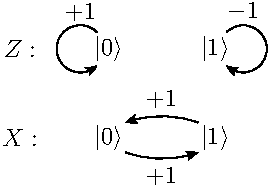
\includegraphics[]{pic-zx.pdf}
\end{center}
From this picture we can see that $Z$ acts by \emph{stabilizing} the
state $\ket{0}$ and anti-stabilizing the $\ket{1}$ state.
The $Z$ operator has been reduced 
to two operators each acting on a one dimensional subspace:
$Z = +1 \oplus -1.$
The $X$ operator serves to ``bitflip'' the state between
these two subspaces.

But what happens if we get confused and end up swapping
the $X$ and $Z$ operators? We would like to see the $X$ operator
as stabilizing / anti-stabilizing two subspaces, together with the
$Z$ operator as bitflipping between these.
The trick is to consider the \emph{orbits} of the operator
we hope to act as a stabilizer.
In this case there is only one orbit, $\ket{0}+\ket{1}$
and indeed, the $Z$ operator bitflips this to another state
$\ket{0}-\ket{1}$ that is anti-stabilized by $X.$

We are going to be considering Hamiltonians built from
summing operators of this form.
In this paper we use a ``neg-Hamiltonian'' convention,
to save complicating expressions with negative signs.
The ground space corresponds to the \emph{largest} eigenvalue.

Building a Hamiltonian from a single $X$ or $Z$ term
we can find the ground space as the stabilized space
using orbits. Then the adjacent operator acts to bitflip
between the eigenspaces.
To further elucidate this idea we turn to another example.
Now we have a hamiltonian built from three commuting and
independent operators 
$$
    \Ham = XXI + IXX + ZZZ.
$$
Starting with $\ket{000}$ we compute the orbit state
as $\ket{000}+\ket{011}+\ket{110}+\ket{101}.$
This time we have three bitflip operators
one for each of the stabilizer operators:
$ZII, IIZ, IXI.$
(We could also have chosen $IZZ, ZZI, XXX.$)
For example, $ZII$ sends the ground state to
$\ket{000}+\ket{011}-\ket{110}-\ket{101}$
which is anti-stabilized by $XXI.$
The bitflip operators form an abelian group of
order $2^3 = 8$ and by appying each element of
this group to the ground state we get a basis
of our state space, which we call a \emph{symmetry
invariant basis.}

Now we consider a four qubit example:
$$
    \Ham = XXII + IIXX + ZIZI + IZIZ.
$$
This time the terms of the Hamiltonian do not form
an abelian group.
We will call the group generated by the terms in the Hamiltonian
the \emph{gauge} group, $G$.
The stabilizers in this case will be the elements of $G$
that commute with every other element in $G.$
By inspection we see these are generated by $\Stab_0=\{XXXX, ZZZZ\}.$
and we can choose the reduced gauge generators to be $R_0=\{XXII, ZIZI\}.$
The logical operators are generated by $L_0 = \{XIXI, ZZII\},$
and then the errors $T_0$ corresponding to $\Stab_0$ will
be $\{ZZZI, IIIX\}.$
All of this can be summarized in a table of anti-commuting pairs:
\begin{center}
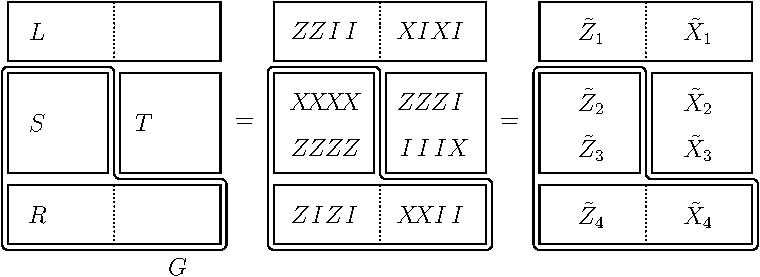
\includegraphics[]{pic-gauge4.pdf}
\end{center}
where the number of rows equals $n$ and each entry
commutes with the entries on other rows, and anticommutes
with the entry on the same row. 
If we take all the operators in the left column
we get the operators 
$\{ ZZII, XXXX, ZZZZ, ZIZI \}.$ 
These generate an abelian group 
that stabilizes the
state $\ket{\psi} = \ket{0000}+\ket{1111}.$
Let $r$ be the gauge operator $XXII$ adjacent to the 
stabilizer $ZIZI$,
The state $\ket{\psi}$ then lies in the $G-$orbit 
$$
\{\ket{\psi}, r\ket{\psi}\} = \{\ket{0000}+\ket{1111}, \ket{1100}+\ket{0011}\}.
$$
We use the $T_0$ operators $t_1=ZZZI$ and $t_2=IIIX$
to list three other $G-$orbits:
$$
\{t_1 \ket{\psi}, t_1 r\ket{\psi}\}, 
\{t_2 \ket{\psi}, t_2 r\ket{\psi}\}, 
\{t_1 t_2 \ket{\psi}, t_1 t_2 r\ket{\psi}\}.
$$
Here we have sixteen vectors forming an orthogonal basis for the state space.
They are arranged on the vertices of a cube. This cube is actually a four
dimensional hypercube, but we suppress the last dimension in
this diagram.
Such an arrangement of basis vectors has a cartesian product
structure which induces a tensor product decomposition of
the original state space.
\begin{center}
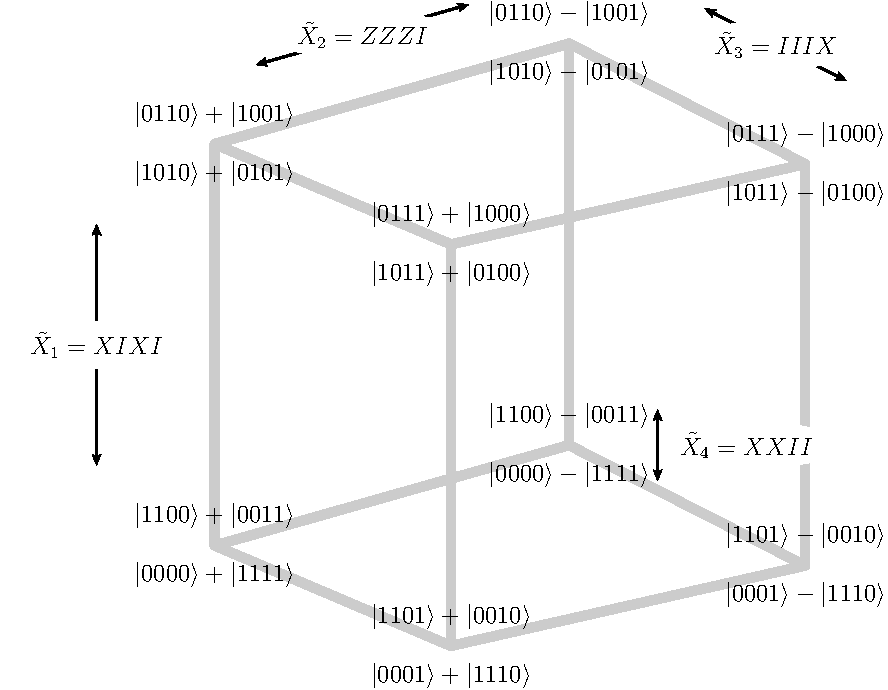
\includegraphics[width=0.7\columnwidth]{pic-operators.pdf}
\end{center}
The Hamiltonian acts on states by left multiplication.
Because this action
is a sum of gauge group elements,
it will decompose into blocks,
one for each $G-$orbit.
We depict this action as a weighted graph, where we omit edges
with zero weight:
\begin{center}
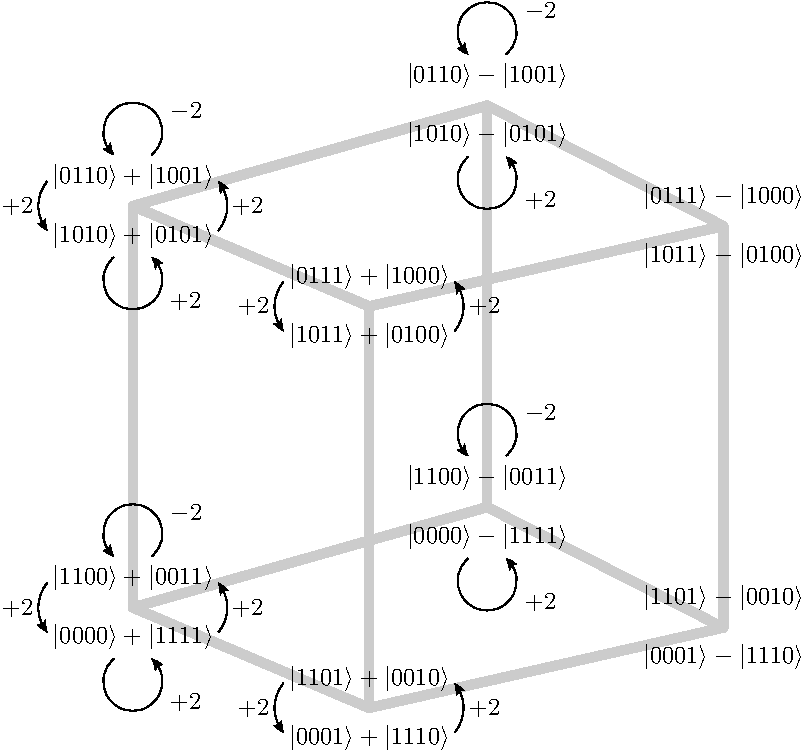
\includegraphics[width=0.7\columnwidth]{pic-orbit.pdf}
\end{center}

\def\Xt{\tilde{X}}
\def\Zt{\tilde{Z}}

\todo{XXX and now for another formula}
\begin{align*}
\Ham &= XXII + IIXX + ZIZI + IZIZ \\
  &= \Xt_4 + \Zt_2\Xt_4 + \Zt_4 + \Zt_3\Zt_4 \\
  &= (I+\Zt_2)\Xt_4 + (I+\Zt_3) \Zt_4.
\end{align*}

Using the symmetry invariant basis computed from the orbits we
can write the matrix for the Hamiltonian in
block diagonal form:
$$
\Ham = 
\left( \begin{array}{cccc}
2(X+Z) & 0 & 0 & 0 \\
0  & 2X & 0 & 0 \\
0  & 0 & 2Z & 0 \\
0  & 0 & 0 & 0 \\
\end{array} \right) \otimes I
$$

\section{Group theoretic representations}

\subsection{The Pauli group}

The Pauli group $\Pauli_1$ is normally 
defined as a set of matrices closed under
matrix multiplication, but we can define
it abstractly
as the group generated
by the (abstract) elements $\{\omega, X, Z\}$ with
relations as follows:
$$
\omega^2=I,\ X^2=I,\ Z^2=I,\ \omega X\omega X=I,\ \omega Z\omega Z=I,\ \mbox{and}\  \omega ZXZX=I,
$$
where $I$ is the group idenity.
Actually, $\omega $ is generated by $X$ and $Z$, so
it is not necessary to include $\omega $ in the generating set,
but here it simplifies the relations.
%\footnote{We leave out $Y$ because...}
This group has eight elements, and is isomorphic to the dihedral group $D_4$,
the symmetry group of a square.

To define
the {\it $n$-qubit Pauli group} $\Pauli_n$, 
we use the $2n+1$ element 
generating set 
$$\{\omega , X_1, .., X_n, Z_1, .., Z_n\}$$
with relation $\omega^2=I$ as before, and
\begin{equation}\label{presentation}
\begin{array}{c}
X_i^2=I,\ Z_i^2=I,\ \omega X_i\omega X_i=I,\ \omega Z_i\omega Z_i=I,\ \omega Z_iX_iZ_iX_i=I, 
\mbox{\ for\ } i=1,...n,\\
Z_iX_jZ_iX_j=I, \mbox{\ for\ } i, j = 1,..,n,\ i\ne j.
\end{array}
\end{equation}

This abstract approach to the definition of a group is known as
a group \emph{presentation}. In general, this is a set of
generators together with a set of relations satisfied
by these generators.

Note that each of the generators squares to the identity,
and of these, only $\omega$ commutes with every element of $\Pauli_n.$
%Note that $\omega$ commutes with all elements of $\Pauli_n$
%and squares to the idenity, 
Therefore we will write $\omega$ as $-I,$
similarly $\pm I$ will denote the
set $\{\omega, I\},$ and $-X$ is $\omega X$, etc.

We write the group commutator as
$[[g, h]]:=ghg^{-1}h^{-1}$
and note the important commutation relation:
$$
    [[Z_i, X_j]] = 
    \left\{ \begin{array}{ll}
 -I &\mbox{if}\ i=j,\\
 I &\mbox{if}\ i\ne j.\end{array}\right.
$$
If we take an arbitrary $g\in \Pauli_n$
written as a product of the generators,
it follows that we can rewrite this
product uniquely as %in an ordered fashion:
$ g = \pm g_1 ... g_n $
where each $g_i$ is one of $I, Z_i, X_i$ or $X_i Z_i$
for $i=1,..,n.$
Therefore, the size of the
Pauli group is 
$$
    |\Pauli_n| = 2^{2n+1}.
$$

%Elements of $\Pauli_n$ that consist of
%products of only $I$ or $X$ will
%be call $X$-type elements (or operators)
%and similarly $Z$-type elements are 
%products of only $I$ or $Z$.
The subgroup of $\Pauli_n$ generated by
the elements $\{X_1,...,X_n\}$ % $\{X_i\}_{i=1,..,n}$ 
is denoted $\Pauli_n^X.$ These are the $X$-type
elements. Similarly,
 $\{Z_1,...,Z_n\}$ generates % $\{Z_i\}_{i=1,..,n}$ 
the subgroup of $Z$-type elements $\Pauli_n^Z$.

\subsection{Subgroups of the Pauli group}

We now define an {\it $n-$qubit gauge group} to be 
any non-abelian subgroup $G$ of $\Pauli_n,$
defined by a set of generators $G_0\subset \Pauli_n,$
%for some subgroup $G$ of $\Pauli_n:$
$$ G := \langle G_0\rangle.$$
%We will assume $G$ is not abelian, which 
%%is equivalent to the condition that $-I\in G.$ % No! {-I, I} is abelian...
%implies that $-I\in G.$
Because $G$ is not abelian, it follows that $-I\in G.$
We also restrict $G_0$ to only contain Hermitian operators,
which is equivalent to requiring that $g^2=I$ for all $g\in G_0.$

Now let $\Stab$ be the largest subgroup of $G$ not containing
$-I.$
$\Stab$ is then an abelian subgroup,
also known as the {\it stabilizer} subgroup.
%(Note that each of the stabilizers commutes with the Hamiltonian.)
$G$ decomposes as a direct product:
$$G = \Stab\times R,$$
where $R\cong P_r$ for some $1\le r\le n,$
and $\Stab\cong \Z_2^{m}$ for $0\le m<n.$
Therefore, 
$$|G| = |\Stab| |R| = 2^{m+2r+1}.$$
We call $R$ the {\it reduced gauge group}.
We consider both $\Stab$ and $R$ to be subgroups of $G.$
%Let $\phi:P_r\to R$ be a group isomorphism,
Let $\phi:R\to P_r$ be a group isomorphism,
%then $R_0 := \{\phi(X_i), \phi(Z_i)\}_{1\le i\le r}$
%then $R_0 := \{\phi(X_i), \phi(Z_i)\}_{i=1,..,r}$
then $R_0 := \{\phi^{-1}(X_i), \phi^{-1}(Z_i)\}_{i=1,..,r}$
is a set of independent generators of $R.$
We also let $\Stab_0$ be a set of $m$ independent generators of $\Stab.$

To find the cosets of $G$ in $\Pauli_n$ we take
the group closure of $G-\Pauli_n$; when this is non-empty
we only need to add $I$ and $-I.$
This is another
gauge group, whose reduced gauge group is known as
the {\it logical} operators $L$, and whose 
stabilizer subgroup is known as the {\it error} operators $T.$
Now any coset of $G$ can be written as $ltG$ with
$l\in L$ and $t\in T.$
The size of $T$ equals the size of $\Stab$: $|T|=|\Stab|=2^m.$
If we let $L_0$ be an independent generating set for $L$
then we have the important formula:
\begin{align}
n &= \frac{1}{2}|L_0| + |\Stab_0| + \frac{1}{2}|R_0|\\
  &= k + m + r
\end{align}
We summarize the information in this section in a table
of Pauli group elements arranged in
two columns and $n$ rows:
\begin{center}
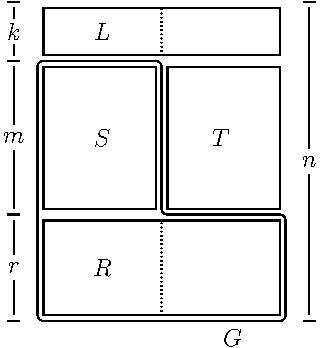
\includegraphics[]{pic-canonical.pdf}
\end{center}
Here we show the $2n$ generators of $\Pauli_n$ arranged 
so that each row contains a pair of generators,
where each such generator anti-commutes with the operator on the same row and
commutes with all the other operators in the table.
Note that this is exactly the definition of the Pauli group
via a presentation given in the previous section.
Furthermore, the table shows $2k$ generators
of $L$, $m$ generators each for $S$ and $T,$ and $2r$
generators of $R.$
The gauge group $G$ encloses $R$ and $S$, and one can
immediately see how $L$ and $T$ also form a gauge group.


\subsection{Representations of the Pauli group}

We now define the
{\it Pauli representation} 
of the Pauli group as a group homomorphism:
$$
    \rho_{\mathrm{pauli}} : \Pauli_n \to \GL(\Complex[2^n])
$$
where $\Complex[2^n]$ is the $2^n$-dimensional state space of $n$ qubits.
On the independent generators 
$\{X_1, .., X_n, Z_1, .., Z_n\},\ \rho_{\mathrm{pauli}}$
is defined as the following tensor product of $2\times 2$ matrices:

%$$
%\rho_{\mathrm{pauli}}(X_i) := \bigotimes_{j=1}^n \left\{ \begin{array}{ll}
%\left( \begin{array}{ll}
%1&0\\
%0&1\end{array} \right) &\mbox{for $j\ne i$,}\\
%\\
%\left( \begin{array}{ll}
%0&1\\
%1&0\end{array} \right) &\mbox{for $j=i$} \end{array}
%\right\},\ 
%\rho_{\mathrm{pauli}}(Z_i) := \bigotimes_{j=1}^n \left\{ \begin{array}{ll}
%\left( \begin{array}{ll}
%1&0\\
%0&1\end{array} \right) &\mbox{for $j\ne i$,}\\
%\\
%\left( \begin{array}{rr}
%1&0\\
%0&-1\end{array} \right) &\mbox{for $j=i$}\end{array}
%\right\}.
%$$

\begin{align*}
\rho_{\mathrm{pauli}}(X_i) := &\bigotimes_{j=1}^n \left\{ \begin{array}{ll}
\left( \begin{array}{ll}
0&1\\
1&0\end{array} \right) &\mbox{for $j=i$}\\
\\
\left( \begin{array}{ll}
1&0\\
0&1\end{array} \right) &\mbox{for $j\ne i$} \end{array}
\right.\\
\rho_{\mathrm{pauli}}(Z_i) := &\bigotimes_{j=1}^n \left\{ \begin{array}{ll}
\left( \begin{array}{ll}
1&0\\
0&-1\end{array} \right) &\mbox{for $j=i$}\\
\\
\left( \begin{array}{rr}
1&0\\
0&1\end{array} \right) &\mbox{for $j\ne i$}\end{array}
\right.
\end{align*}

%on $n$ qubits, $\Pauli_n,$
%as the set of $n$-fold tensor products
%of the matrices $\pm I, X, Z:$
%$$
%I = \left( \begin{array}{ll}
%1&0\\
%0&1\end{array} \right),\quad
%X = \left( \begin{array}{ll}
%0&1\\
%1&0\end{array} \right),\quad
%Z = \left( \begin{array}{ll}
%1&0\\
%0&-1\end{array} \right).
%$$

Normally the image of 
$\rho_{\mathrm{pauli}}$ is thought of as the
Pauli group itself, and we are indeed free to think
that way because $\rho_{\mathrm{pauli}}$ is a group
isomorphism.

Given a group representation $\rho:G\to GL(V)$
the {\it character} of $\rho$ is a function
$\chi_\rho:G\to \Complex$ given by
$$
    \chi_\rho(g) = \mbox{Tr}\ \rho(g).
$$

Given two functions $u,v : G \to \Complex$ 
we define the following inner product:
$$
    \langle u, v \rangle := \frac{1}{|G|} \sum_{g\in G} u(g) \overline{v(g)}.
$$

The character of the Pauli representation, $\chi_{{pauli}}:\Pauli_n\to\Complex$
is given by:
$$
\chi_{{pauli}}(g) = \sum_{v \in basis} \langle v | \rho_{{pauli}}(g) | v \rangle
    = \left\{ \begin{array}{ll}
 \pm 2^n &\mbox{if}\ g=\pm I\\
 0 &\mbox{otherwise}\end{array}\right.
$$

Since $|P_n|=2^{2n+1}$ it follows that
$\langle\chi_{pauli},\chi_{pauli}\rangle = 1$ and
so $\rho_{pauli}$ is an irreducible representation of $\Pauli_n.$

%It turns out %(see Appendix for details)
%that $\rho_{\mathrm{pauli}}$ is an
%irreducible representation ({\it irrep}) of $\Pauli_n$. 
The only other irreps of $\Pauli_n$ are 
the $1$-dimensional irreps $\rho:\Pauli_n\to\Complex$
defined on the independent generators as:
    $$ \rho(X_i) = \pm 1,\quad \rho(Z_i) = \pm 1.$$

So we have $2^{2n}$ many $1$-dimensional irreps,
and a single $2^n$-dimensional irrep.
Summing the squares of the dimensions
shows that we have a complete set of irreps of $\Pauli_n.$

%\subsection{Representations of stabilizer groups}
%
%Any abelian subgroup $\Stab\subset \Pauli_n$
%that does not contain $-I$ we call a stabilizer group.
%The reason for this name is...


\subsection{Representations of gauge groups}

%Our next job will be to find the irreps of {\it subgroups} of $\Pauli_n.$
Although $\rho_{\mathrm{pauli}}$
restricted to a gauge group $G\subset\Pauli_n$ serves as a representation
of $G$ it is no longer irreducible.
Our aim will be to decompose $\rho_{\mathrm{pauli}}$ into irreps of $G.$

The $1$-dimensional irreps $\rho:G\to \Complex,$
are now defined by
specifying the action of $\rho$ on the independent generators:
$$
    \rho(h)=\pm 1\ \mbox{for}\ h\in \Stab_0,
    \quad \rho(\phi^{-1}(X_i)) = \pm 1,\quad \rho(\phi^{-1}(Z_i)) = \pm 1.
$$
This gives all $2^{m+2r}$ of the $1$-dimensional irreps.
%These will turn out not to be used below.

The $2^r$-dimensional irreps are given by:
$$
    \rho(h) = \pm I^{\otimes r}\ \mbox{for}\ h\in \Stab_0,
    \quad \rho(\phi^{-1}(X_i)) = X_i,\quad \rho(\phi^{-1}(Z_i)) = Z_i.
$$
We are free to choose the signs of the $\rho(h)$ for each $h\in \Stab_0.$
Hence there are $2^m$ many of these irreps.
Each such choice corresponds to the choice of a {\it syndrome} vector $s(h)=\pm 1$, for $h \in \Stab_0,$
or alternatively, choice of an element $t\in T:$
$$
    \rho^1_t(h) = \left\{ \begin{array}{ll}
 I^{\otimes r}\ &\mbox{if $th=ht$}\\
 -I^{\otimes r}\ &\mbox{if $th=-ht$}\end{array} \right. %\right\}\mbox{for}\ h\in \Stab_0.
$$

%Finally, there are $2^m$ many $2^r$-dimensional irreps $\rho_t$
%which are labeled by $t\in T$ and defined as
%$$
%    %\rho_t(h)=\pm I^{\otimes 2^r}\ \mbox{for}\ h\in \Stab_0,
%    %\rho_t(h)= [t,h] = th^{-1}th^{-1} = \pm I^{\otimes 2^r}\ \mbox{for}\ h\in \Stab_0,
%    \rho_t(h) = \left\{ \begin{array}{ll}
% I^{\otimes 2^r}\ &\mbox{if $th=ht$}\\
% -I^{\otimes 2^r}\ &\mbox{if $th=-ht$}\end{array} \right\}\mbox{for}\ h\in \Stab_0,
%    \quad \rho_t(\phi^{-1}(X_i)) = X_i,\quad \rho_t(\phi^{-1}(Z_i)) = Z_i.
%$$

%For $G$ a subgroup of $\Pauli_n$, and decomposition
Because $G$ decomposes 
into a direct product $G=\Stab\times \Pauli_r$ we have the
following representations:
$$
    \rho_t(g) = \rho^1_t(h) \rho^r_{pauli}(g'),
$$
where $g=hg'$, $h\in \Stab$, $g'\in \Pauli_r$ 
%and $\rho_1(h)$ is a $1$-dimensional representation of $\Stab$.
and $\rho^r_{pauli}$ is the $r$-qubit Pauli representation.
The character for this representation is:
$$
\chi_{t}(hg') = \rho_t^1(h) \sum_{v \in basis} \langle v | \rho^r_{{pauli}}(g') | v \rangle
    = \left\{ \begin{array}{ll}
 \pm 2^r\rho_t^1(h) &\mbox{if}\ g'=\pm I\\
 0 &\mbox{otherwise}\end{array}\right.
$$

We have that $|G|=2^{2r+m+1}$ and so
$\langle\chi_{t},\chi_{t}\rangle = 1$ and
$\rho_t$ is an irreducible representation of $G.$
We now count the occurances of 
this representation in $\rho^r_{pauli}$:
\begin{align*}
\langle\chi^r_{pauli},\chi_{t}\rangle &= \frac{1}{|G|}\sum_{g\in G} \chi^r_{pauli}(g)\overline{\chi_{t}(g)} \\
&= \frac{1}{2^{2r+m+1}} \sum_{g=\pm I} 2^n 2^r = \frac{2^{n+1+r}}{2^{2r+m+1}} = 2^k
\end{align*}
where $k$ is the number of logical qubits so that $n=r+m+k.$

%\noindent{\bf Theorem.}
%Using characters one can show that
%on a subgroup $G$ of $\Pauli_n$ the
In summary, the Pauli representation decomposes into 
$2^m$ many irreps $\rho_t,$ 
each with dimension $2^r,$ 
and appearing with multiplicity $2^k:$
$$
    \rho_{\mathrm{pauli}} = 
        \bigoplus_{t\in T}\ \rho_t \otimes I^{\otimes k}
$$
%where we label the $2^r$-dimensional irreps by $t\in T.$
%See appendix for details.

\subsection{Symmetry invariant basis}

In general, given a representation $\rho:G\to \GL(V)$
and the character of some irreducible representation $\chi:G\to \C$
the following operator 
$P:V\to V$
projects onto the subspace on which
this irreducible representation acts:
$$
    P := \frac{d}{|G|} \sum_{g\in G} {\overline{\chi(g)}} \rho(g).
$$
where $d$ is the dimension of the irreducible representation.
We can use this to calculate projectors onto the irreps $\rho_t$ in $\rho_{pauli}$:
\begin{align*}
P_t &= \frac{d}{|G|} \sum_{g\in G} \overline{\chi_t(g)} \rho_{pauli}(g) \\
    &= \frac{d}{|G|} \sum_{h\in \Stab}\sum_{g\in R} \overline{\chi_t(hg)} \rho_{pauli}(hg) \\
    &= \frac{d}{|G|} 2^{2r} \sum_{h\in \Stab} {\rho^1_t(h)} \rho_{pauli}(h) \\
    &= \frac{1}{2^m} \sum_{h\in \Stab} {\rho^1_t(h)} \rho_{pauli}(h).
\end{align*}

We can also write this as a product of projectors onto
the $\pm 1$ eigenspaces of stabilizers $\rho_{pauli}(h)$ for $h\in \Stab.$
Choose generators $h_1,...,h_m$ of $S$
and then the projectors onto the $\pm 1$ eigenspace of $\rho_{pauli}(h_i)$ are
$$
P^i_t = \frac{1}{2} \bigl(I^{\otimes n} \pm \rho_{pauli}(h_i) \bigr)
$$
and we see that 
$$
P_t = \prod_{i=1,...,m} P^i_t 
    = \frac{1}{2^m} \bigl(I^{\otimes n} \pm \rho_{pauli}(h_1)\bigr)
    ...\bigl(I^{\otimes n} \pm \rho_{pauli}(h_m)\bigr).
$$
This projector will have rank $2^{k+r}$ and
$$
U := \sum_{t\in T} P_t
$$
is a unitary transformation that sends
physical qubits to encoded qubits.


\subsection{The Hamiltonian}

The Hamiltonian of interest is 
an operator $\Ham:\Complex[2^n]\to\Complex[2^n]$:
%and normally defined
%as the negative sum of terms from $G_0,$ but here
%we will reverse the sign:
$$ \Ham := \sum_{g\in G_0} \rho_{\mathrm{pauli}}(g).$$
Using the above decomposition we find:
\begin{align*}
    \Ham &= \sum_{g\in G_0}\ \bigoplus_{l\in L, t\in T}\ \rho_t(g)\\
         &= \bigoplus_{l\in L, t\in T} \sum_{g\in G_0}\ \rho_t(g).
\end{align*}
%The goal is to decompose $\Ham$ into blocks as
%$$
%    \Ham = \bigoplus_{\mathrm{irrep}\rho} \sum_{g\in G_0}\ \rho(g),
%$$
We will notate each block as
$\Ham_t := \sum_{g\in G_0}\rho_t(g)$
for each irrep $\rho_t$ appearing in $\Ham.$
\begin{framed}
\noindent{\bf Fact 0:}
The Hamiltonian is block diagonalized, with blocks indexed by operators $t$ in
the abelian group $T$ and multiplicity $2^k:$
$$
    \Ham =  \bigoplus_{t\in T}\ \Ham_t \otimes I^{\otimes k}.
$$
\end{framed}
%Writing $I$ for the identity element of $T$ we write the corresponding
%block of the hamiltonian as $\Ham_{0,0}.$

More generally, we can assign real valued weights
$J_g\in\R$
to each operator $g\in G_0,$
\begin{align*}
    \Ham = \sum_{g\in G_0} J_g \rho_{\mathrm{pauli}}(g)
            = \bigoplus_{l\in L, t\in T} \sum_{g\in G_0}\ J_g \rho_t(g).
\end{align*}
In other words, using weights does not change the block structure of $\Ham.$

In the following sections we will forget the distinction 
between $g$ and $\rho_{\mathrm{pauli}}(g)$,
so terms such as $Z$ and $X$ can be understood
as the corresponding Pauli linear operators.

%%%%%%%%%%%%%%%%%%%%%%%%%%%%%%%%%%%%%%%%%%%%%%%%%%%%%%%%%%%%%%%%%%%%%%%%%%%%%%%
%
%%%%%%%%%%%%%%%%%%%%%%%%%%%%%%%%%%%%%%%%%%%%%%%%%%%%%%%%%%%%%%%%%%%%%%%%%%%%%%%
%

\section{Applications}

We now use the tools built so far
to analyse two examples of gauge code Hamiltonians.
The above procedure is not entirely automatic,
it relies on extracting the isomorphism $\phi$,
but when this can be made to work it works surprisingly well.

%%%%%%%%%%%%%%%%%%%%%%%%%%%%%%%%%%%%%%%%%%%%%%%%%%%%%%%%%%%%%%%%%%%%%%%%%%%%%%%
%
%%%%%%%%%%%%%%%%%%%%%%%%%%%%%%%%%%%%%%%%%%%%%%%%%%%%%%%%%%%%%%%%%%%%%%%%%%%%%%%
%

\subsection{The 2D compass model}

Here we consider the two-dimensional compass model \cite{Bacon2006}.
We coordinatize the qubits on a square 
lattice of\ $l\times l$\ sites,
$(i, j)$\ for\ $1\le i, j\le l.$
This gives $n = l^2.$
For the single qubit Pauli operators acting on site
$(i, j)$ we coordinatize with subscripts $ij$, 
with $i$ and $j$ understood modulo $l$.
The generators of the gauge group are
$$
    G_0 = \big\{ X_{ij}X_{i,j+1},\ Z_{ij}Z_{i+1,j}\ \mbox{for}\ 1\le i, j\le l\big\}.
$$
We write generators of the reduced
gauge group in anti-commuting pairs:
$$
    R_0 = \big\{ X_{i1}X_{ij},\ Z_{1j}Z_{ij}\ \mbox{for}\ 2\le i, j\le l\big\}.
$$
This makes it clear the isomorphism $\phi : R \to \Pauli_r$ to use,
and we again use pairs $i,j$ to coordinatize $\Pauli_r$:
$$
    \phi(X_{i1}X_{ij}) = X_{i-1,j-1}, \ \ \phi(Z_{1j}Z_{ij}) = Z_{i-1,j-1},\ \mbox{for}\ 2\le i, j\le l.
$$
The generators for the stabilizers are
$$
    \Stab_0 = \big\{ \prod_{i=1}^l X_{ij}X_{i,j+1},\ \prod_{i=1}^l Z_{ji}Z_{j+1,i}\ \mbox{for}\ 1\le j\le l-1\big\}.
$$
The logical operators are generated by $L_0 = \big\{ \prod_i X_{i1}, \prod_j Z_{1j} \}.$
These sets have cardinalities:
$$|G_0|=2l^2,\ |R_0| = 2(l-1)^2,\ |\Stab_0| = 2(l-1).$$
%And we note that $\frac{1}{2}|L_0| + |\Stab_0| + \frac{1}{2}|R_0| = n.$
And we note that $k+m+r=n$ is satisfied.
%Now we can define the irreps of $G$.
Now we write down the values of the
irreps on the gauge operators.
Here we define each irrep using a pair 
of syndrome vectors $s_X$ and $s_Z:$
\begin{align*}
\rho(X_{i1} X_{i2}) &= X_{i-1,1} &
%\rho(Z_{1i} Z_{2i}) &= Z_{1,i-1} &\mbox{for}\ 2\le i\le l\\
\rho(Z_{1i} Z_{2i}) &= Z_{1,i-1} \\&&&\mbox{for}\ 2\le i\le l\\
\rho(X_{il} X_{i1}) &= X_{i-1,l-1} &
%\rho(Z_{li} Z_{1i}) &= Z_{l-1,i-1} &\mbox{for}\ 2\le i\le l\\
\rho(Z_{li} Z_{1i}) &= Z_{l-1,i-1} \\&&&\mbox{for}\ 2\le i\le l\\
\rho(X_{ij} X_{i,j+1}) &= X_{i-1,j-1} X_{i-1,j} &
%\rho(Z_{ji} Z_{j,i+1}) &= Z_{j-1,i-1}Z_{j,i-1} &\mbox{for}\ 2\le i\le l, 2\le j<l\\
\rho(Z_{ji} Z_{j,i+1}) &= Z_{j-1,i-1}Z_{j,i-1} \\&&&\mbox{for}\ 2\le i\le l, 2\le j<l\\
\rho(X_{1j} X_{1,j+1}) &= s_X(j-1) \prod_{i=1}^{l-1} X_{i,j-1} X_{ij} &
%\rho(Z_{j1} Z_{j+1,1}) &= s_Z(j-1) \prod_{i=1}^{l-1} Z_{j-1,i} Z_{ji} &\mbox{for}\ 2\le j<l\\
\rho(Z_{j1} Z_{j+1,1}) &= s_Z(j-1) \prod_{i=1}^{l-1} Z_{j-1,i} Z_{ji} \\&&&\mbox{for}\ 2\le j<l\\
\rho(X_{11} X_{12}) &= \prod_{j=1}^{l-1}s_X(j) \prod_{i=1}^{l-1} X_{i1} &
\rho(Z_{11} Z_{21}) &= \prod_{j=1}^{l-1}s_Z(j) \prod_{i=1}^{l-1} Z_{1i}.
\end{align*}
Note the transposition symmetry between the $X$ and $Z$-type operators.
We sum all these terms to find 
the form of the hamiltonian in each block:
$$
\Ham_\rho = \sum_{g\in G_0} \rho(g) = \sum_{1\le i,j<l} \rho(X_{ij}X_{i,j+1}) + \rho(Z_{ij}Z_{i+1,j}).
$$
We note that in \cite{Brzezicki2013},
they perform a
spin transformation of the compass model
which also results in an $(l-1)\times(l-1)$ lattice
of spins and identical Hamiltonian up to some signs.

%Note that the form of each of the Hamiltonian blocks $H_t$
%comes from another gauge code.
%In this case it has some non-local operators, as well as $\pm 1$ factors
%which can be subsumed into the gauge code as operators $\pm I.$

%We have the following important fact which we will prove in section \ref{spectra} below:
%\begin{framed}
%\noindent{\bf Fact 1:}
%The blocks $H_t$ of a CSS gauge code Hamiltonian are also CSS.
%\end{framed}
%
%By counting dimensions we can conclude the following:
%\begin{framed}
%\noindent{\bf Fact 2:}
%Each block $H_t$ has non-degenerate groundspace.
%\end{framed}
%
%\emph{!! check what happens with weights $\pm 1.$}

%\fbox{\parbox[b]{5cm}{This is long text that will be wrapped once it reaches five centimeters.}}

%%%%%%%%%%%%%%%%%%%%%%%%%%%%%%%%%%%%%%%%%%%%%%%%%%%%%%%%%%%%%%%%%%%%%%%%%%%%%%%
%

\subsection{The 1D $XY$-model}

This example shares features of both the previous and the next examples.
The $XY$-model lives on a one dimensional chain of $n$ qubits.
We write the gauge group generators as
$$
    G_0 = \{ X_i X_{i+1}, Z_i Z_{i+1} \ \mbox{for}\ i=1,...,n \}
$$
with periodic boundary conditions.

Normally these operators are written as 
$\{ X_i X_{i+1}, Y_i Y_{i+1} \ \mbox{for}\ i=1,...,n \}$
but note that there is an automorphism of the Pauli group...
\todo{XXX}


%%%%%%%%%%%%%%%%%%%%%%%%%%%%%%%%%%%%%%%%%%%%%%%%%%%%%%%%%%%%%%%%%%%%%%%%%%%%%%%
%

\subsection{The Kitaev honeycomb model}


%\begin{figure*}[th!]
%\begin{center}
%        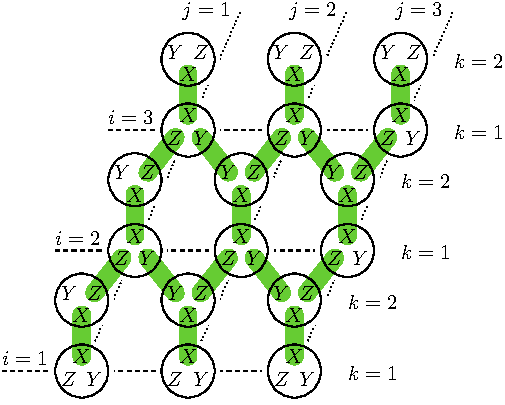
\includegraphics[width=0.6\columnwidth]{fig_00.pdf}
%\caption{
%Gauge generators have support on the edges of the honeycomb lattice.
%Qubits here are depicted as circles.
%}
%\label{honeycomb}
%\end{center}
%\end{figure*}


The Kitaev honeycomb model \cite{Kitaev2006} is built from spins on
the sites of a hexagonal lattice. 
The lattice of linear size $l$ has $n=2l^2$ sites
which we coordinatize using integer triples $i, j, k$
with $1\le j, k\le l$ and $k=1, 2.$
We use periodic boundary conditions so $i, j$ are
to be taken modulo $l$.
Gauge generators have support on the edges of the honeycomb lattice,
and we depict qubits here as circles:
\begin{center}
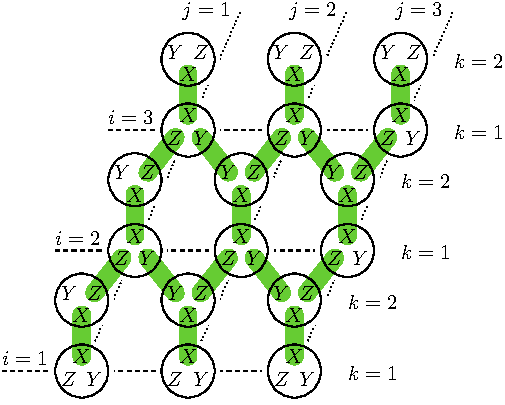
\includegraphics[width=0.6\columnwidth]{fig_00.pdf}
\end{center}
%See figure \ref{honeycomb}.
The edges of the lattice are in one-to-one
correspondence with the generators $G_0$:
$$
G_0 := \big\{X_{ij1}X_{ij2},\ Z_{ij2}Z_{i+1,j1},\ Y_{ij1}Y_{i-1,j+1,2}
\ \mbox{for}\ 1\le i,j\le l\big\}.
$$
Note that we make the definition $Y:=XZ$ for each site.

Stabilizers are generated from closed strings of
gauge operators. 
For example, each hexagon gives a stabilizer
\begin{align*}
h_{ij}:&= 
X_{ij1}X_{ij2}
Z_{ij2}Z_{i+1,j1}
Y_{i+1,j1}Y_{i,j+1,2}
X_{i,j+1,2}X_{i,j+1,1}
Z_{i,j+1,1}Z_{i-1,j+1,2}
Y_{i-1,j+1,2}Y_{ij1}
\\
&= 
Z_{ij1} Y_{ij2} X_{i+1,j1}
Z_{i,j+1,2} Y_{i,j+1,1} X_{i-1,j+1,2}.
\end{align*}

And the two homologically non-trivial loops
give stabilizers:
$$
h_v := \prod_{i=1}^l Y_{i11} Y_{i12},\ \ 
h_h := \prod_{j=1}^l X_{1j2} X_{2j1}.
$$

This gives independent stabilizer generators $\Stab_0$
from each hexagon, less one, as well as $h_v$ and $h_h.$
%two homologically non-trivial loops.
The number of hexagons is $\frac{1}{2}n$ and
so we find $|\Stab_0|=\half n+1.$
There are no logical operators, so we
must have $|R_0|=n-2.$

%\begin{figure*}[th!]
%\begin{center}
%        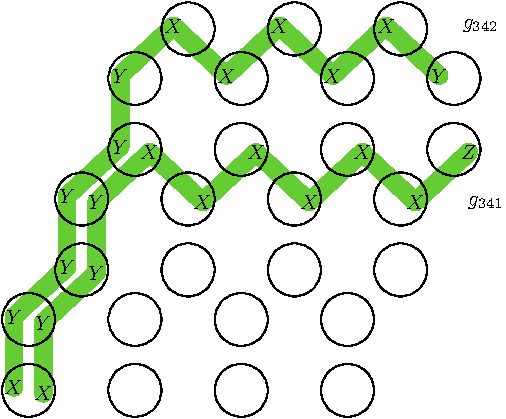
\includegraphics[width=0.5\columnwidth]{fig_01.pdf}
%%\caption{Two elements $g_{341}$ and $g_{342}$ of the set $R_0$}
%\caption{Two elements of the set $R_0$ corresponding
%to $i=3$, $j=4$ and $k=1,2.$}
%\label{jaws}
%\end{center}
%\end{figure*}

Now we construct a set of string operators $R_0$,
one for each site on the lattice, except for
the two sites $(1,1,1)$ and $(1,1,2).$
Each string $g_{ijk}\in R_0$
is constructed as the product of
gauge operators along a path starting at
$(1,1,1)$ and terminating at $(i,j,k).$
%See figure \ref{jaws}.

Two elements of the set $R_0$ corresponding
to $i=3$, $j=4$ and $k=1,2.$
\begin{center}
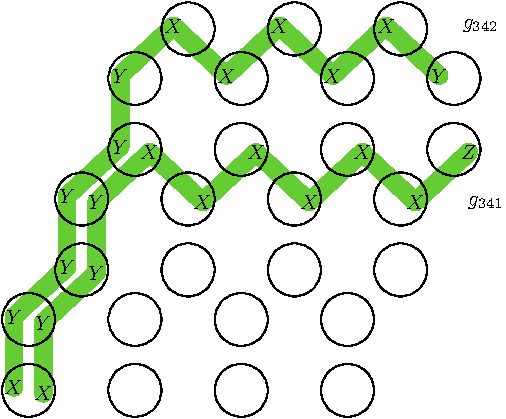
\includegraphics[width=0.5\columnwidth]{fig_01.pdf}
\end{center}

Each such path is built from two ``straight''
path segments, first in the $i$ direction
and then in the $j$ direction. 
The paths for operators $g_{ij1}$ and
$g_{ij2}$ coincide along the $i$ direction
but become disjoint in the $j$ direction:
the $g_{ij1}$ path goes around the bottom
of the hexagons and the $g_{ij2}$ path
goes around the top.
With periodic boundary conditions $R_0$ forms an
independent generating set of $R$ of size $n-2.$

We construct an isomorphism $\phi: R\to \Pauli_r$
by sending elements of $R_0$ bijectively
to the following independent generating
set of $\Pauli_r$:
$$
\big\{c_{2j}:=Z_1...Z_{j-1} X_j,\ c_{2j+1}:=Z_1...Z_{j-1} Y_j\ \ \mbox{for}\ 1\le j\le r\big\}.
$$
The bijection is constrained 
by setting $\phi(g_{ij1}):=c_{2j'+1}$
and $\phi(g_{ij2}):=c_{2j'}$
where $j'$ is chosen uniquely for each $i, j.$
The $c_j$ are paired Majorana fermion operators \cite{Kitaev2006}.

%We construct an isomorphism $\phi: R\to \Pauli_r$
%by setting $\phi(g_{ij1}):=c_{2j'}$
%and $\phi(g_{ij2}):=c_{2j'+1}$
%%we map 
%%elements of $R_0$ to the following independent generating
%where the $c_j$ form the following independent generating
%set of $\Pauli_r$:
%$$
%%\big\{\prod_{i=1}^{j-1} Z_i X_j,\ \prod_{i=1}^{j-1} Z_i Y_j\ \mbox{for}\ 1\le j\le r\big\}.
%\big\{c_{2j}:=Z_1...Z_{j-1} X_j,\ c_{2j+1}:=Z_1...Z_{j-1} Y_j\ \ \mbox{for}\ 1\le j\le r\big\}.
%$$

We check this is a group homomorphism by showing that relations
satisfied by elements of $R_0$ are satisfied by
their images under $\phi.$
All such relations are either of the form
$g^2=~\pm~I$, $gg'=\pm~g'g$, or
products thereof.
So it is sufficient to check squares of
elements and commutation relations.
Every element of $R_0$ anticommutes with
every other element of $R_0$, and this is true also
of the $c_j.$
Also, $g_{ij1}^2=-I$ and $g_{ij2}^2=I$ 
is preserved by $\phi$ because $c_{2j}^2=I$ and $c_{2j+1}^2=-I$.
Finally, $\phi$ is an isomorphism
because it is a bijection of two independent
generating sets.

The next step is to write each element of $G_0$
as a product of reduced gauge operators and stabilizers.
The key thing to note is that the product of two
operators $g_{ijk}, g_{i'j'k'}\in R_0$ gives a string
operator between the sites $(i,j,k)$ and $(i',j',k')$.
And {\it any} string operator between these
two sites can then be generated by using stabilizers to
``deform'' the string $g_{ijk}g_{i'j'k'}.$
For example, taking the product
of two operators from $R_0$ that differ
by one path segment gives the following:
\begin{align*}
Z_{ij2}Z_{i+1,j,1} &= g_{ij2} g_{i+1,j,1} \\
%&\mbox{for}\ \  1\le i<l,\ 1\le j\le l, \ \ \mbox{except}\ \  (i,j)=(1,1) \ \ \mbox{or}\ \ (l,1)\\
Y_{i+1,j,1}Y_{i,j+1,2} &= g_{i+1,j,1}g_{i,j+1,2}
%&\mbox{for}\ \  1\le i,j\le l, \ \ \mbox{except}\ \  (i,j)=(1,1) \ \ \mbox{or}\ \ (l,1).
\end{align*}
We need the homologically non-trivial stabilizers to get these:
\begin{align*}
Z_{lj2}Z_{1j1} &= h_v g_{lj2} g_{1j1} &\mbox{for}\ \  2\le j\le l
\end{align*}
And the $X_{ij1}X_{ij2}$
gauge operators can be generated
by the product of 
$g_{ij1}g_{ij2}$ and the enclosed hexagon stabilizers:
$$X_{ij1}X_{ij2}=g_{ij1}g_{ij2}\prod_{j'=1}^{j-1} h_{ij'}.$$

The only $G_0$ operators that are not 
quadratic in $R_0$ operators are the five
operators that touch either of the sites
$(1,1,1)$ or $(1,1,2)$.

So each block in the Hamiltonian
is seen to be quadratic in the $c_j$ plus
five other Pauli operator terms which we denote as $\Lambda_\rho$:
$$
    \Ham_\rho = \sum_{ij} \Gamma_{ij}(\rho) c_i c_j + \Lambda_\rho
$$
The coefficients $\Gamma_{ij}$ are dependant on the irrep $\rho.$

In \cite{Kells2009} they introduce a similar set of
mutually anti-commuting string operators $R_0.$

%A similar analysis applies to the ising model, Jordan-Wigner... 
%http://arxiv.org/pdf/1504.01444 page 86.

%%%%%%%%%%%%%%%%%%%%%%%%%%%%%%%%%%%%%%%%%%%%%%%%%%%%%%%%%%%%%%%%%%%%%%%%%%%%%%%
%

\def\Cn{\Complex[2^n]}
\def\Cr{\Complex[2^r]}
%\def\Field{\mathcal{F}_2}
\def\Field{\mathcal{F}}
%\def\Fn{\Field[n]}
%\def\Fr{\Field[r]}
\def\Fn{\Field^n}
\def\Fm{\Field^m}
\def\Fr{\Field^r}
%\def\Fnd{\Field^{n*}}
%\def\Fmd{\Field^{m*}}
%\def\Frd{\Field^{r*}}
\def\Fnd{\Field_{n}}
\def\Fmd{\Field_{m}}
\def\Frd{\Field_{r}}

\def\Im{\mathrm{im}}
\def\Ker{\mathrm{ker}}
%\def\Span#1{\mathrm{span}(#1)}
\def\Span#1{\langle #1 \rangle}

%\section{Representations over the finite field $\Field$}
\section{Symplectic representations}

This is a way of ``brute-forcing'' the representations when
we cannot find a way of writing them down in a closed form expression.
For finite systems this yields an algorithm that is efficiently implementable.

In this section, and the remainder of this chapter,
we restrict our
attention to gauge groups formed from terms 
in $\Pauli_n^X\cup\Pauli_n^Z.$
We call these \emph{CSS gauge codes.}
We briefly review the symplectic structure of
these operators.

Let $\Field$ denote the finite field with two elements $0$ and $1$.
Both $\Pauli^X_n$ and $\Pauli^Z_n$ are abelian groups,
and can be identified with the additive 
group structure of the $n$ dimensional vector space
over $\Field:$
$$
    \Pauli^X_n \cong \Fn,  \ \ 
    \Pauli^Z_n \cong \Fn. 
$$
We do this in the obvious way by sending $X_i$ to the basis vector with
$1$ in the $i-$th entry, and similarly for each $Z_i$. 
We also identify the computational basis of our statespace $\Complex[2^n]$
with $\Fn$ in the obvious way:
$$
\Complex[2^n] \cong \Complex[\Fn].
$$
This has the potential to be very confusing, and
so where appropriate we use $X$ and $Z$ subscripts.
%apart from occasionally
%we resist the temptation to
%use any other decorations.

$X$-type operators act on the $\Complex[\Fn]$
basis vectors using $\Field$ addition:
$$
    g_X \in \Pauli^X_n \cong \Fn, \ \ g_X : v \longmapsto g_X + v
$$

$Z$-type operators act on the
$\Complex[\Fn]$ basis vectors using $\Field$ inner product:
$$
    g_Z \in \Pauli^Z_n \cong \Fn, \ \ g_Z : v^\top \longmapsto g_Z v^\top
$$
This is an $\Field$ scalar, just zero or one. We think of this
as a ``syndrome''.
This suggests that actually these $Z$-type operators
live in the dual vector space $\Fnd.$
Because of the underlying symmetry
(and notational confusion)
between the $X$ and $Z$-type operators,
we make the convention that by default
all our $\Field$-vectors come as row vectors (ie. dual vectors).
This means we use the transpose operator $^\top$ to
indicate a primal (column) vector.
%so a product $u v^\top$ of
%two $\Fn$ vectors is a scalar.

It doesn't make sense to add an $X$-type operator and
a $Z$-type operator:
$$
    g_Z + g_X \ \ \ \mbox{\emph{no no!!!}}
$$
but it does make sense to take the inner product:
$$
    g_Z g_X^\top = g_X g_Z^\top.
$$
This is an $\Field$ scalar which gives the commutator of the 
two operators.

An $\Field$-linear operator such as
$ A : \Fn \to \Fm $
acts on the left as $ u^\top \mapsto A u^\top.$
It also acts on dual vectors as
$ A : \Fmd \to \Fnd $
which corresponds to acting on the right: $v \mapsto vA.$ 
We call the rowspace of 
$A$ the \emph{span} and denote 
it as 
$$\Span{A} = \{ vA | v \in \Fmd \}$$
The kernel of $A$ is defined as
$$
    \Ker(A) = \{ u^\top | u^\top \in \Fn,\ \  A u^\top = 0 \}.
$$

We wish to use this language to decompose a CSS gauge group $G.$
First we write the gauge group generators in terms of
$X$-type and $Z$-type operators:
$$
    G_0 = G_X \cup G_Z.
$$
Following the theory from the previous section,
we are going to rewrite the gauge group generators
as a union of stabilizer generators $S_0 = S_X \cup S_Z$
and reduced gauge generators $R_0 = R_X \cup R_Z.$
Similarly, the error operators
will be split into $X$ and $Z$ type
operators $T_X$ and $T_Z$ and
finally the logical operators
$L_X$ and $L_Z.$
We summarize all of these sets
in the following table:
\begin{center}
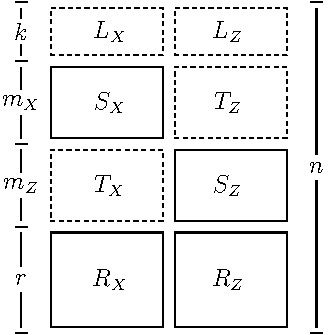
\includegraphics[]{pic-symplectic.pdf}
\end{center}
The solid rectangles indicate operators that
span the $X$ and $Z$ parts of the gauge group,
and the dashed rectangles indicate operators that
do not live inside the guage group.

We consider each of these blocks 
$L_X, L_Z, S_X, T_Z, T_X, S_Z, R_X, R_Z,$
as well as $G_X,G_Z,$
%Each of these blocks can be thought of as 
as either a set of $\Fnd$ vectors (the rows) or as an 
$\Field$-linear operator.
For example, we write $u\in R_X$ to mean $u$ is 
a row of the matrix $R_X$.
%As an $r\times n$ matrix this operator is
%$$
%    R_X : \Field^n] \to \Field^r]
%$$
%Given $v\in \Fr$ then $u = v R_X$ is
%a generic vector in the rowspace of $R_X.$

We first find the stabilizers $S_Z$.
These are built out of $\Fnd$ vectors from the span of $G_Z$
that commute with the rows of $G_X:$
\begin{align*}
    \Span{S_Z} &= \{\  vG_Z \ |\  v G_Z G_X^\top = 0, \ \ v \in F_{|G_Z|}\ \} \\
               &= \{\  vG_Z \ |\  v^\top \in \Ker(G_X G_Z^\top)  \ \}.
\end{align*}
The generators (rows of $S_Z$) are then extracted
from this span by row reduction.
We swap the role of $X$ and $Z$ to find $S_X.$

Once we have the stabilizers, in order to
complete the above table as a presentation
of the Pauli group we solve the
following $\Field$-linear block matrix equation,
%All of this can be summarized in the block matrix equation:
$$
\left( \begin{array}{l}
L_X\\
S_X\\
T_X\\
R_X
\end{array} \right)
\left( \begin{array}{l}
L_Z\\
T_Z\\
S_Z\\
R_Z
\end{array} \right)^\top =
I,
$$
%And once again we have a presentation of the Pauli group.
subject to the restriction that the rows of
$R_X$ lie in the span of $G_X$ and
the rows of $L_X$ do not.
Similarly for $R_Z$ and $L_Z.$
This set of 16 equations is quadratic in the unknown variables
and so it is not obvious how to proceed, but it turns out a
systematic way can be found.

We begin by finding $L_Z.$
These operators satisfy the following \emph{homology} condition:
$$
    l_Z \in L_Z \smbox{is given by} l_Z^\top \in \Ker(G_X) \smbox{mod} \Span{S_Z}.
$$
In other words, $L_Z$ is formed from a basis for the kernel of $G_X$ 
row-reduced using $S_Z.$
To be more specific %about this operation of mod $\Span{S_Z}$
we take any direct sum decomposition
$$\Fnd = \Span{S_Z} \oplus V$$
then the operation of mod $\Span{S_Z}$ is the
projection onto $V.$
We can explicitly write such a 
projector as the $n\times n$
matrix given by
$$
    P_Z = I + A^\top S_Z
$$
where the matrix $A$ is the $m_Z\times n$ matrix consisting of
the leading 1's in any row-reduction of $S_Z.$
We define $P_X$ similarly for the operation of mod $\Span{S_X}.$

To find $L_X$ we solve the following $\Field$-linear
system:
%\begin{align*}
%    L_Z L_X^\top &= I, \\
%    G_Z L_X^\top &= 0.
%\end{align*}
$$
\left( \begin{array}{l}
L_Z\\
G_Z\\
\end{array} \right)
L_X^\top = 
\left( \begin{array}{l}
I\\
0
\end{array} \right)
$$

The reduced gauge group matrix $R_X$
is found as a row-reduction of $G_X P_X.$
We cannot merely set $R_Z$ to be $G_Z P_Z$ 
because we also require $R_X R_Z^\top = I.$
Instead we define the auxiliary matrix
$\widetilde{R}_Z$ to be a row-reduction of  $G_Z P_Z.$

The error operators $T_X$ are then found as the solution
to the $\Field$-linear system:
%\begin{align*}
%    S_Z T_X^\top &= I,\\
%    L_Z T_X^\top &= 0,\\
%    \widetilde{R}_Z T_X^\top &= 0.
%\end{align*}
$$
\left( \begin{array}{l}
L_Z\\
S_Z\\
\widetilde{R}_Z
\end{array} \right)
T_X^\top = 
\left( \begin{array}{l}
0\\
I\\
0
\end{array} \right)
$$
And then the operators $T_Z$ solve the $\Field$-linear system:
%\begin{align*}
%    S_X T_Z^\top &= I,\\
%    T_X T_Z^\top &= 0,\\
%    L_X T_Z^\top &= 0,\\
%    R_X T_Z^\top &= 0.
%\end{align*}
$$
\left( \begin{array}{l}
L_X\\
S_X\\
T_X\\
R_X
\end{array} \right)
T_Z^\top = 
\left( \begin{array}{l}
0\\
I\\
0\\
0
\end{array} \right)
$$
Finally at this point $R_Z$ is given as the solution to
%\begin{align*}
%    R_X R_Z^\top &= I,\\
%    L_X R_Z^\top &= 0,\\
%    S_X R_Z^\top &= 0,\\
%    T_X R_Z^\top &= 0.
%\end{align*}
$$
\left( \begin{array}{l}
L_X\\
S_X\\
T_X\\
R_X
\end{array} \right)
R_Z^\top = 
\left( \begin{array}{l}
0\\
0\\
0\\
I
\end{array} \right)
$$
Note that $R_Z$ and $\widetilde{R}_Z$ have identicle span 
and so we have $R_Z T_X^\top = 0.$

We call this array of eight $\Field$-linear 
matrices
an $(L,S,T,R)$-decomposition of the gauge group.
In general this will not be unique for
any given gauge group.

\subsection{The Hamiltonian}

The complex Hilbert state space of our
Hamiltonian has $2^n$ dimensions and we
write this space as $\Complex[2^n]$.
This notation is meant to suggest that
we are forming a $\Complex$ vector space
using $2^n$ ``points'' 
as basis vectors.
Working in the computational basis,
we do indeed have $2^n$ such points; 
these are the elements of $\Fnd.$
And so we make the identification
$$
    \Complex[2^n] \cong \Complex[\Fnd].
$$
In other words, we are labeling 
our basis vectors with elements of $\Fnd$
and therefore such notation as
$$
    \bra{u} H \ket{v}
$$
with $u, v \in \Fnd$ makes sense.
We will make further use of this below,
by writing  $\Field$-vector space 
computations inside the Dirac brakets.

Returning to the code $(L,S,T,R)$-decomposition
above,
given the Pauli operator $t\in T$ such that $t = t_X t_Z$ (in $\Pauli_n$)
we get a basis for the irrep $\rho_t$:
$$
    \{ \ket{v R_X + t_X} \ \mbox{such that}\  v \in \Frd \}.
$$
In other words,
the basis of the irrep $\rho_t$ is 
an affine subspace of $\Fnd.$
Each such affine subspace is indexed by an
element of $\Frd$ and
all of these are
translates of each other,
so we make the following identification:
$$
\Complex[\{vR_X+t_X\}_{v\in\Frd}]
\cong \Complex[\Frd].
$$
This will allow us to write the components
of each block $H_t$ of the Hamiltonian
as $\bra{u}H_t\ket{v}$ for $u,v\in\Frd.$
We make this identification of affine subspaces
not out of laziness but because it will
help us to compare each of
the Hamiltonian blocks $H_t$ below.

\begin{framed}
\noindent{\bf Important:}
The computational basis identifies
basis vectors of $\Complex[2^n]$
with elements of a finite vector space $\Fnd$:
$$
    \Complex[2^n] \cong \Complex[\Fnd].
$$
The $(L,S,T,R)$-decomposition naturally
decomposes $\Fnd$ into $2^{m_Z+k}$ affine subspaces:
$$
    \{ v R_X + t_X + l_X \}_{v\in\Frd}
$$
for each $t_X \in \Span{T_X}, l_X \in \Span{L_X}.$
Each such affine subspace forms a basis
for the irreducible blocks $H_{t_X,t_Z}$ of $H$,
and can be naturally identified with $\Frd:$
$$
    H_{t_X,t_Z} : \Complex[\Frd] \to \Complex[\Frd].
$$
\end{framed}

We now wish to understand the action of the
gauge group on each of its irreps.
Starting with the $t_X,t_Z=0,0$ irrep,
this is where each of the stabilizers has
a trivial action. 
In $\Fn$ this
corresponds to the additive action of the zero vector.

\newcommand{\pluseq}{\mathrel{+}=}
States $u\in\Span{R_X}$ can be built from a
vector matrix product
$$
    u = v R_X
$$
with $v\in\Frd.$
Since $R_X R_Z^\top = I$
we can write $v = u R_Z^\top.$
Each $g_X\in G_X$ acts on $u$ to give
\begin{align*}
    u_1 &= (u + g_X) \ \mbox{mod}\ \Span{S_X} \\
        &= (u + g_X) P_X \\
        &= (v R_X + g_X) P_X.
\end{align*}
writing $u_1 = v_1 R_X$ we then have
\begin{align*}
    v_1 &= (v R_X + g_X) P_X R_Z^\top \\
        &= v + g_X R_Z^\top.
\end{align*}
%\todo{XXX explain that \todo{$P_X R_Z^\top = R_Z^\top$} etc. XXX}
So we have that working in the computational
basis, the action of the $X$ part of the
gauge group in the $t_X,t_Z=0,0$ irrep is to send
%$v\in R_X$ to 
$v\in \Frd$ to $v + g_X R_Z^\top.$
In summary, we have the following contributions from the
$G_X$ terms of the Hamiltonian:
$$
%    H_{0,0}(v, v+g_X  R_Z^\top) \ne 0,\ \ \mbox{for}\ g_X\in G_X, v\in \Frd
    \bra{v} H_{0,0} \ket{v+g_X  R_Z^\top} 
        \pluseq 1,\ \ \mbox{for}\ g_X\in G_X, v\in \Frd
$$
where we use the $\pluseq$ notation
because there may be other contributions to the
same component.
These terms will always be off
the diagonal unless $g_X$ is a stabilizer.

The action of the $G_Z$ gauge group
contributes to the diagonal of $H.$
These diagonal terms apply a kind of
``potential energy'' penalty
to the basis states
that depends on the \emph{syndrome} vector:
$$
    \mbox{syndrome}(u) = G_Z u^\top
$$
for $u^\top \in \Fn.$
This is an $\Field$-vector that has one component for
each row of $G_Z.$
Writing $|G_Z|$ for the number of these rows, and 
using a \emph{weight} function $w$ that just counts
the number of non-zero entries in any $\Field$-vector
we have the following contributions to
the Hamiltonian:
$$
    \bra{v} H_{0,0} \ket{v} 
        \pluseq |G_Z| - 2w(G_Z R_X^\top v^\top),
$$
for $v\in \Frd.$

Adding up all of the above we
have in summary,
$$
H_{0,0} = \sum_{\substack{v\in\Frd\\g_X\in G_X } }
  \ket{v+g_X  R_Z^\top}\bra{v} 
  + \sum_{v\in\Frd} \bigl(|G_Z| - 2w(G_Z R_X^\top v^\top)
    \bigr) \ \ket{v}\bra{v}.
$$

For any $t_X\in \Span{T_X}$ the Hamiltonian block $H_{t_X,0}$
has components indexed by basis vectors:
$$
    u = v R_X + t_X
$$
this means that the $G_X$ gauge terms
have the same effect on $H_{t_X,0}$
as $H_{0,0}$ and only the diagonal has changed:
$$
H_{t_X,0} = \sum_{\substack{v\in\Frd\\g_X\in G_X } }
  \ket{v+g_X  R_Z^\top}\bra{v} 
  + \sum_{v\in\Frd} \bigl(
    |G_Z| - 2w(G_Z R_X^\top v^\top + G_Z t_X^\top)
    \bigr) \ \ket{v}\bra{v}.
$$
%Writing the difference explicitly:
%$$
%    H_{0,0} - H_{t_X,0} = 
%  \sum_{v\in\Frd} 2\bigl(
%    w(G_Z R_X^\top v^\top + G_Z t_X^\top)
%    -w(G_Z R_X^\top v^\top)
%    \bigr) \ \ket{v}\bra{v}.
%$$
The general form of
each the Hamiltonian block is:
\begin{align*}
H_{t_X,t_Z} = &\sum_{\substack{v\in\Frd\\g_X\in G_X } }
    \eta(t_Z g_X^\top)
  \ \ket{v+g_X  R_Z^\top}\bra{v} \\
  &+ \sum_{v\in\Frd} \bigl(
    |G_Z| - 2w(G_Z R_X^\top v^\top + G_Z t_X^\top)
    \bigr) \ \ket{v}\bra{v}.
\end{align*}
Here we use $\eta$ to send 
$t_Zg_X^\top$ which is an $\Field$ value
to the multiplicative subgroup $\{\pm1\}$
of $\Complex:$
$$
    \eta(0) = 1,\ \eta(1) = -1.
$$
The $\eta(t_Zg_X^\top)$ term
is a kind of parity check that
picks up one phase flip for (some of)
the $X$ type stabilizers found in $g_X.$
This works because $T_Z$ is a left inverse
of $S_X^\top.$
The $t_Z\in\Span{T_Z}$ selects which
$X$ type stabilizers act as $-1$ in this irrep.

In summary, we have the complete representation
theory for $CSS$ gauge code Hamiltonians.
%It is a remarkable fact that this involves such
%a close interplay with $\Field$ linear algebra.


%%%%%%%%%%%%%%%%%%%%%%%%%%%%%%%%%%%%%%%%%%%%%%%%%%%%%%%%%%%%%%%%%%%%%%%%%%%%%%%
%

\section{Perron-Frobenius theory}

%We restrict our attention to Hamiltonians whose off-diagonal entries
%are non-negative (in some basis).
%These are also known as \emph{stoquastic} Hamiltonians \cite{Bravyi2006}.
%This can be achieved by considering Hamiltonians where each term
%involves either $X$-type operators or $Z$-type operators but not both.
%That is, $G_0$ consists only of $X$-type operators and $Z$-type operators.
%We will call this a \emph{CSS gauge code Hamiltonian} after the stabilizer codes
%of the same name.
%We also shift the Hamiltonian by a constant energy, so that
%the diagonal entries are non-negative:
%$$
%%\Ham := \sum_{g\in G_0} \rho_{\mathrm{pauli}}(g).
%\Ham := \sum_{g\in G_0} \rho_{\mathrm{pauli}}(g) + kI.
%$$
%This does not change the spectral gap or eigenvectors.

%This is another kind of representation theory of $\Pauli_n.$
%We are representing either $G_X$ or $G_Z$ as a permutation representation (?)
%It has the ability to extract irreps of $G$ corresponding to
%the $X$ type operators as affine subspaces $\{vR_X+t\}$ of $\Fn.$
%For the $Z$ representations we will still need the complex
%representation theory to build states on $\Complex[\{vR_X+t\}]$
%that look like ``waves''.
%These (stationary) waves do indeed have a geometric interpretation,
%with the wavefront nodes being identified with so-called Cheeger cuts.
%To switch back and forth between the $X$ and $Z$ type
%representations 

We begin this section with the following two definitions.
A CSS gauge code is \emph{self-dual} when the $X$ and $Z$ type
gauge generators are equal: $$G_X = G_Z.$$
The $XY$-model is an example of a self-dual code.
A CSS gauge code is \emph{weakly self-dual}
when there is a permutation $P$ on the set of $n$ qubits
that induces equality of the gauge generators:
$$
    G_X P = G_Z,
$$
where we write $P$ as an $n\times n$ permutation matrix.
The compass model is then weakly self-dual when we transpose
the square lattice of $l\times l$ qubits.

We now turn to another notion of reducibility, coarser than
the group theoretic reducibility.
The easiest way to understand this is via graph theory.
Given a CSS gauge code Hamiltonian $H,$ 
we see that 
the diagonal terms (working in the computational basis)
come from the $Z$ operators and the off-diagonal terms
come from $X$ type operators.
\todo{...stoquastic...}
This suggests the following definition.
We define a graph $\Gamma$ with vertices the $2^n$ computational
basis elements, and edges:
$$
    \ket{v} \mapsto g_X \ket{v}, \smbox{for all} v\in\Fnd, g_X\in G_X.
$$
These are undirected edges because $g_X^2 = I.$
We also add weighted loops corresponding to the $Z$-type gauge operators:
$$
    \ket{v} \mapsto \sum_{g_Z\in G_Z} g_Z \ket{v}, \smbox{for all} v\in\Fnd.
$$
In this way we can consider $H$ and $\Gamma$ interchangeably,
as either a matrix or a graph.
An irreducible matrix is one whose corresponding graph is connected.
Using the $\Field$-linear $(L,S,T,R)$-decomposition of the gauge group
we then have the following:
\begin{framed}
\noindent In the computational basis, any CSS gauge code
Hamiltonian $H$ is the direct sum of $2^{m_Z}$
irreducible matrices $\Gamma_{t_X}$
indexed by $t_X\in\Span{T_X}$
with multiplicity $2^k$:
$$
    H = \bigoplus_{
    \substack{t_X\in\Span{T_X}\\l_X\in\Span{L_X}}}
        \Gamma_{t_X}.
$$
\end{framed}
A basis for each $\Gamma_{t_X}$ is given by a coset
of $G_X$ in $\Fnd:$
$$
    \{ v S_X + u R_X + t_X \}_{v\in \Field_{m_X}, u\in\Frd}.
$$

%See \cite{Baez2012}
%We return to the investigation of Hamiltonians
%formed from CSS gauge codes.
%We can think of such Hamiltonians as the adjacency matrix of a graph.
%Loosely speaking we can view the off-diagonal terms as 
%raising and lowering operators, and the diagonal
%terms measure the energy of each level.

The off-diagonal entries of $H$ are all positive.
If we use a spectral shift operator, a constant multiple of the identity $+cI$,
we find that $H+cI$ is a non-negative matrix. 
We call such a matrix \emph{Perron-Frobenius.}
%Now we invoke the Peron-Frobenius theorem.
Each of the blocks $\Gamma_{t_X}$ is also Perron-Frobenius
and in combination with their irreducibility this means the following:
\begin{framed}
\noindent For each $t_X\in\Span{T_X}$
the largest eigenvalue 
of $\Gamma_{t_X},$
$$\lambda_1(\Gamma_{t_X})
$$
is non-degenerate,
and is associated with an eigenvector 
$$v_1(\Gamma_{t_X})
$$
with positive components.
\end{framed}
\todo{PF theorem}

Now we make the restriction that $H$
comes from a weakly self-dual gauge code.
Our goal will be to show that the
groundspace of $H$ is spanned
by vectors which are stabilized.
This will imply that $\lambda_1(H)=\lambda_1(H_{0,0}).$
To begin, let $v_1$ be the top
eigenvector of $\Gamma_{t_X}$ with $t_X\in\Span{T_X}.$
Because $v_1$ has all positive components
it will be fixed by  any operator
$s\in\Span{S_Z}$.
To show that the $X$ type stabilizers
also fix $v_1$ 
we use weak self-duality
and see that by change of basis
we can swap the roles of the $X$ and $Z$ type operators.
\begin{framed}
\noindent{\bf Fact 1:}

For any weakly self-dual gauge code Hamiltonian $\Ham$
every groundstate is stabilized 
and so $$\lambda_1(\Ham) = \lambda_1(\Ham_{0,0})$$
and for $t_X\in\Span{T_X}, t_Z\in\Span{T_Z}$
with $t_X\ne 0$ or $t_Z\ne 0$
$$
\lambda_1(\Ham) > \lambda_1(H_{t_X,t_Z}).
$$
\end{framed}
Notice that 
$H_{0,0}$ is also Perron-Frobenius (in the computational basis)
and so has non-degenerate
groundspace, but it appears with multiplicity $2^k$ within
the Hamiltonian $H$ and this accounts for the degeneracy of the
groundspace of $H$.

%Taken together, these eigenvectors form a basis for the
%groundspace of the system.
%Stabilizers act as $+1$ or $-1$ on eigenvectors
%of the Hamiltonian.
%A stabilizer $s\in\Pauli^X$ just permutes the
%coordinates of the groundstate and so must fix any
%groundstate. 
%A stabilizer $s\in\Pauli^Z$ acts trivially
%on $\ket{0...0}$ and therefore must also fix any groundstate.
%We have demonstrated the following

%A simple variational argument % ???
%shows that the top eigenvector (the groundstate)
%can be chosen to have all positive entries
%(this is the Perron-Frobenius theorem)
%and therefore is stabilized:

The next goal is to search for
the second eigenvalue of $H$,
$\lambda_2(H).$
Using a basis change and the
above equation for $H_{t_X,0}$
we have
\begin{framed}
\noindent{\bf Fact 2:}
Given a weakly self-dual
gauge code Hamiltonian $\Ham$ and
$t_X\in \Span{T_X},\  t_X\in \Span{T_Z}$
the blocks $\Ham_{t_X,0}$ and 
$\Ham_{0,t_Z}$ are Perron-Frobenius.
\end{framed}

We extend the above argument:
\begin{framed}
\noindent For a weakly self-dual gauge code
Hamiltonian,
and $t_X\ne 0$, $t_Z\ne 0$
\begin{align*}
\lambda_1(\Ham_{t_X,0}) &< 
    \lambda_1(\Ham_{t_X,t_Z}) \ \smbox{and}\\
\lambda_1(\Ham_{0,t_Z}) &< 
    \lambda_1(\Ham_{t_X,t_Z}).
\end{align*}
\end{framed}

In summary, 
to find the spectral gap of a weakly self-dual Hamiltonian,
which is the difference of the top two eigenvalues of the Hamiltonian,
we need only examine the top two eigenvalues of $H_{0,0}$ and 
the top eigenvalue of $H_{t_X,0}$ for each $t_X\in T_X.$ 

\section{The gauge color code model}

%\begin{center}
%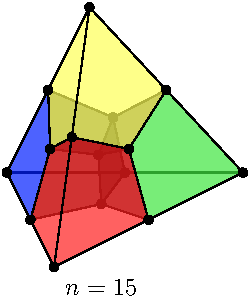
\includegraphics[width=0.3\columnwidth]{pic-gcolor-1.pdf}
%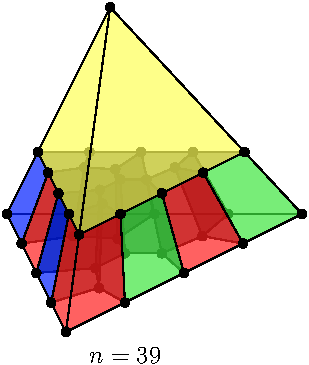
\includegraphics[width=0.3\columnwidth]{pic-gcolor-15.pdf}
%\end{center}
%
%\begin{center}
%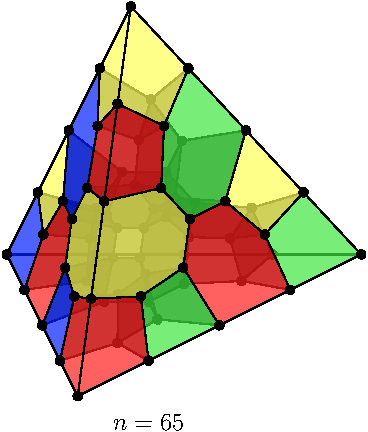
\includegraphics[width=0.3\columnwidth]{pic-gcolor-2.pdf}
%\end{center}

We now turn to the central animal that motivated
the theory developed in this chapter.


The three dimensional gauge color code \cite{Bombin2015,Bombin2015single,Kubica2015}
is a self-dual CSS gauge code. 
It is based on the following geometric construction known
as a \emph{colex} \cite{Bombin2007exact}.
We begin with a tetrahedron and subdivide it into finitely many
convex 3-dimensional polytopes, or \emph{bodies}.
Each body has a boundary consisting of 0-dimensional cells
which we call \emph{vertices}, 1-dimensional cells called \emph{edges}
and 2-dimensional cells called \emph{faces}.
By a \emph{cell} we mean any of these 0,1,2 or 3-dimensional convex polytopes.
Any two bodies in this tetrahedral subdivision will
have either empty intersection or otherwise intersect
on a common vertex, edge or face.
When the intersection is on a face these two bodies
are called \emph{adjacent}.
Two vertices in the same edge will also be called adjacent.
Each body is colored by one of four \emph{colors},
either taken to be red, green, blue, yellow or 
otherwise an element of the set $\{1, 2, 3, 4\}.$
The four exterior triangular faces of the bounding tetrahedron are
called \emph{regions,} the intersection of two regions is called
a \emph{border} and the intersection of three regions is called
a \emph{corner.}
A cell not contained within any region is called an interior cell.

This colored cellulation is required to have the following further properties:
\begin{enumerate}
\item Adjacent bodies have different colors.
\item Each region has a unique color 
such that no bodies intersecting that region has that color.
\item All vertices are adjacent to four other vertices,
except for the corner vertices which are adjacent to three other vertices.
\end{enumerate}

Here we show some instances of this construction,
along with the colors of the unobscured bodies.
Each instance is labeled by the number of vertices $n$.
\begin{center}
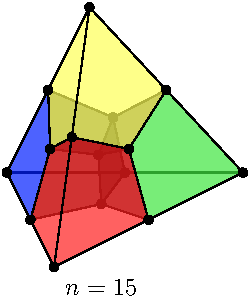
\includegraphics{pic-gcolor-1.pdf}\ \ \ \ \ \ \ \ \ \ \ 
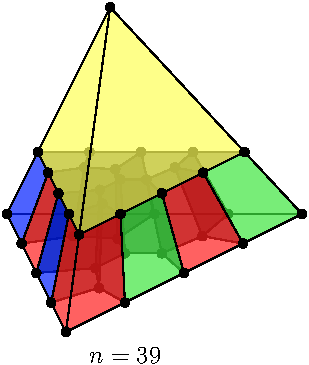
\includegraphics{pic-gcolor-15.pdf}
\end{center}

\begin{center}
\includegraphics{pic-gcolor-2.pdf}\ \ \ \ \ \ \ \ \ \   \includegraphics{pic-gcolor-3.pdf}
\end{center}

%From the above conditions it follows that:\\
We note the following consequences of the above conditions.
Every face supports an even number of vertices.
% Each face cobounds two bodies, the other bodies that
% share an edge must be 2-colorable, ie even number of edges.
We now think of each region as corresponding to a ``missing'' body.
Each edge is then contained in the boundary of three bodies.
%Every interior edge is in the boundary of three bodies.
%Edges contained in the regions are either in the boundary of two bodies or
%otherwise are contained in one of the borders and the boundary of one body.
This means we can associate a unique color to each edge,
which is also the color of two bodies intersecting a vertex of the edge.
That is, each edge joins two bodies of the same color.
Each face bounds two bodies, and so we color each face with the two colors of these bodies.
%We color each face with the two colors of the bodies 

Using this cellulation we now construct the gauge code.
Qubits are associated with the $n$ vertices.
We associate operators to other cells, or union of cells,
by using the contained vertices as support.
Because this is a self-dual code, the same goes for
both the $X$ and $Z$ type operators.
%and we confuse the distinction between union of cells
%and the corresponding $X$ or $Z$ type operator.
The $X/Z-$type gauge group is generated by
$X/Z-$type operators supported on each face.
The $X/Z-$type stabilizer group is generated by
$X/Z-$type operators supported on each body.
There is one $X/Z-$type logical operator and these
are generated by
$X/Z-$type operators supported on any region.

%%%%%%%%%%%%%%%%%%%%%%%%%%%%%%%%%%%%%%%%%%%%%%%%%%%%%%%%%%%%%%%%%%%%%%%%%%%%%%%
%


\section{The orbigraph}

Performing numerics on small gauge code models makes
it evident that there is a great deal more symmetry than
we have found using the above techniques.
In particular, the components of eigenvectors 
have many identical values.
This motivates the following exploration of the symmetry 
of the Hamiltonian.

A graph automorphism is a permutation matrix $P$
such that 
$$P^T \Ham P = \Ham.$$
%Equivalently, $P$ commutes with $\Ham$ and this means it preserves
%the eigenspaces of $\Ham$.
\def\auto{\mathcal{A}}
The set of all such graph automorphisms 
form a group $\auto$.
%form a group $\auto(H)$ or just $\auto$ when the graph is understood.
We now define a new matrix $\Ham//\auto$
that acts on the vector space with basis consisting
of the orbits of $\auto.$
The matrix components of $\Ham//\auto$ will be
indexed by a pair of $\auto-$orbits $i$ and $j$ and have value
$$
    (\Ham//\auto)_{ij} = |\{ g\in G \smbox{s.t.} gv \in j \}| \smbox{where}v\in i.
$$
In other words, 
$(\Ham//\auto)_{ij} $ counts the number of gauge group
elements that sends any particular element $v$ of the 
$\auto-$orbit $i$ to the $\auto-$orbit $j.$

Here is a simple example. % potential only depends on hamming weight: Jarret
We take as gauge group 
$$G = \{XII, IXI, IIX, ZII, IZI, IIZ\}.$$
The Hamiltonian $H = \sum_{g\in G} g$ has matrix:
$$
H = \left(\begin{array}{rrrrrrrr}
 3 &  1 &  1 &  1 &  . &  . &  . &  . \cr
  1 &  1 &  . &  . &  1 &  1 &  . &  . \cr
  1 &  . &  1 &  . &  1 &  . &  1 &  . \cr
  1 &  . &  . &  1 &  . &  1 &  1 &  . \cr
  . &  1 &  1 &  . & -1 &  . &  . &  1 \cr
  . &  1 &  . &  1 &  . & -1 &  . &  1 \cr
  . &  . &  1 &  1 &  . &  . & -1 &  1 \cr
  . &  . &  . &  . &  1 &  1 &  1 & -3
\end{array}\right)
$$
where we indicate zero entries with a dot.
In this case, the automorphism group is $\auto=S_3,$
there are four $\auto-$orbits, and
$$
H//\auto = \left(\begin{array}{rrrr}
 3 &  3 &  . &  . \cr
  1 &  1 &  2 &  . \cr
  . &  2 & -1 &  1 \cr
  . &  . &  3 & -3
\end{array}\right).
$$
In this case the automorphism group $\auto$ of the graph
is the same as the automorphism group $Aut(G)$ of the gauge group,
but in general it is possible that $Aut(G) < \auto.$

Note that the orbigraph is no longer Hermitian,
and in general will not even be normal.

We can also write $H//\auto = QHP$ using the following two matrices for $P$ and $Q:$
$$
Q = 
\left(\begin{array}{rrrrrrrr}
 1 &  . &  . &  . &  . &  . &  . &  . \cr
  . &  1 &  . &  . &  . &  . &  . &  . \cr
  . &  . &  . &  . &  1 &  . &  . &  . \cr
  . &  . &  . &  . &  . &  . &  . &  1
\end{array}\right),\ \ \ 
P = 
\left(\begin{array}{rrrr}
 1 &  . &  . &  . \cr
  . &  1 &  . &  . \cr
  . &  1 &  . &  . \cr
  . &  1 &  . &  . \cr
  . &  . &  1 &  . \cr
  . &  . &  1 &  . \cr
  . &  . &  1 &  . \cr
  . &  . &  . &  1
\end{array}\right).
$$
The idea is that each column of $P$ sums over an orbit,
and each row of $Q$ chooses one member of each orbit.
%See also \cite{Cvetkovic1980} chapter 5.

%The automorphisms of the gauge group, $Aut(G)$ will induce an
%automorphism of the graph by \todo{XXX}...
%In particular, elements of the stabilizer group $\Stab$ induce graph 
%automorphisms by \todo{XXX}...
%In general there may be more symmetry in the graph that
%we cannot access via a group automorphism.

In general, we will apply this idea to each of the blocks $H_{t_X,0}$.
From {\bf Fact 2} above, and using the fact that we are
summing over a trivial representation of $\auto$ we have the following:
\begin{framed}
\noindent{\bf Fact 3:}
The orbigraph of $\Ham_{t_X,0}$ contains the ground eigenvalue of $\Ham_{t_X,0}.$
\end{framed}

%%%%%%%%%%%%%%%%%%%%%%%%%%%%%%%%%%%%%%%%%%%%%%%%%%%%%%%%%%%%%%%%%%%%%%%%%%%%%%%
%
\subsection{The compass model}
For the next example we take the $l=3$ compass model.
$\Ham_{0,0}$ acts on a 16 dimensional space.
The order of $\auto$ is $72$, and we find three $\auto-$orbits.
% This time $Aut(G) = \auto$ ???
The orbigraph method can be applied in the case
where the Hamiltonian weights for $X$ and $Z$ are uniform as $w_X$ and $w_Z.$
We separate the $X$ and $Z$ terms of the orbigraph to show
how this works:
$$
\Ham_{0,0}//\auto = 
\left(\begin{array}{rrr}
 . &  9 &  . \cr
  1 &  4 &  4 \cr
  . &  6 &  3
\end{array}\right) + 
\left(\begin{array}{rrr}
 9 &  . &  . \cr
  . &  1 &  . \cr
  . &  . &  -3
\end{array}\right)
=
\left(\begin{array}{rrr}
 9 &  9 &  . \cr
  1 &  5 &  4 \cr
  . &  6 &  .
\end{array}\right)
$$
This can be solved analytically and we find $\lambda_1 = 4+2\sqrt{13} \cong 11.21110255.$
Keep in mind that the original state space has dimension $2^9=512$ so we
have come a long way down to 3.

By exact%\footnote{Exact in this context means that we do not do any
%perturbative approxiamations to the operator in question.}
numerical diagonalization
we get the spectrum of $\Ham_{0,0}$ and note that the orbigraph lifts
all degeneracy as well as missing some excited eigenspaces:
\begin{center}
\begin{tabular}{ c|c|c } 
$\lambda$ & $\Ham_{0,0}$ degeneracy & $\Ham_{0,0}//\auto$ degeneracy \\
\hline
    11.2111025509 & 1 & 1 \\
    6.0 & 1 & 1 \\
    2.0 & 4 &   \\
    0.0 & 4 &   \\
    -3.21110255093 & 1 & 1 \\
    -4.0 & 4 &   \\
    -6.0 & 1 &   
\end{tabular}
\end{center}
The reason we miss some excited spaces is that they do not contain
any trivial irrep of $\auto.$
Note that we miss the eigenspace with $\lambda = -6$
even though this is one dimensional. It must contain some other non-trivial
one dimensional irrep. 
%This cannot happen with the groundspace because
%those eigenvectors are all positive.
If we want to make an orbigraph for these other spaces we would construct
the orbigraph by
summing over orbits using different characters of $\auto$
(these are \emph{momenta} in the abelian terminology).
See \cite{Cvetkovic1980} chapter 5 for more details.

%%%%%%%%%%%%%%%%%%%%%%%%%%%%%%%%%%%%%%%%%%%%%%%%%%%%%%%%%%%%%%%%%%%%%%%%%%%%%%%
%
\subsection{The gauge color code model}
The smallest gauge color code has $n=15$ qubits,
$G_0$ has $18$ each of X/Z-type gauge operators,
and $4$ each of X/Z-type stabilizer generators.
$\Ham_{0,0}$ acts on a 64 dimensional space, and $\auto$ has
order 720. We find 7 orbits:
$$
\Ham_{0,0}//\auto = 
\left(\begin{array}{rrrrrrr}
18 & 18 &  . &  . &  . &  . &  . \cr
  3 & 12 & 15 &  . &  . &  . &  . \cr
  . &  6 &  6 & 12 &  . &  . &  . \cr
  . &  . &  9 &  . &  9 &  . &  . \cr
  . &  . &  . & 12 & -6 &  6 &  . \cr
  . &  . &  . &  . & 15 & -12 &  3 \cr
  . &  . &  . &  . &  . & 18 & -18
\end{array}\right)
$$
The eigenvalue equation results in
the recurrence relation:
$$
    \lambda a_k = 3ka_{k-1} + (18-6k)a_k + (18-3k)a_{k+1},
$$
which has largest solution 
$\lambda_1 = 18\sqrt{2} \cong 25.4558441.$

% RP^3 is homeomorphic to the solid ball with antipodal points identified
% http://math.stackexchange.com/questions/507783/mathbbrp3-is-homeomorphic-to-the-solid-ball-with-antipodal-points-identifi
% http://topospaces.subwiki.org/wiki/Homology_of_real_projective_space

Numerics give the full spectrum of $\Ham_{0,0}$ and we note that the orbigraph lifts
all degeneracy as well as preserving every eigenvalue:
\begin{center}
\begin{tabular}{ c|c|c } 
$\lambda$ & $\Ham_{0,0}$ degeneracy & $\Ham_{0,0}//\auto$ degeneracy \\
\hline
    25.4558441227 & 1 & 1 \\
    16.9705627485 & 6 & 1 \\
    8.48528137424 & 15 & 1 \\
    0.0 & 20 & 1 \\
    -8.48528137424 & 15 & 1 \\
    -16.9705627485 & 6 & 1 \\
    -25.4558441227 & 1 & 1 \\
\end{tabular}
\end{center}

The second eigenvalue of $H$ comes from a recurrence
relation in two variables which has solution
$\lambda_2 = 9\sqrt{2} + 3\sqrt{10} \cong 22.21475504.$
So the gap for this Hamiltonian  is 
$$\lambda_1 - \lambda_2 = 9\sqrt{2} - 3\sqrt{10} \cong 3.24108908.$$



%%%%%%%%%%%%%%%%%%%%%%%%%%%%%%%%%%%%%%%%%%%%%%%%%%%%%%%%%%%%%%%%%%%%%%%%%%%%%%%
%
\subsection{A table of orbigraphs}

Here we tabulate graph automorphisms of $H_{t_X,0}$
and the resulting orbigraph sizes.
We use the software library {\tt nauty}\cite{McKay2014} for computing graph automorphisms.

\begin{center}
\begin{tabular}{ l|c|c|c|l|c|c|c } 
model &\ $n$\ &\ $r$\ &\ $t_X$\ & $\auto$ & $|\auto|$ & $|\auto-\mathrm{orbits}|$ & 
$|\mathrm{Aut(code)}|$ \\
\hline
%    1D $XY$ & 4 &  2& 0 & 2 & 3 & 8 \\
%       & 5 &  4& 0 & 10 & 4 & 10 \\
%       & 6 &  4& 0 & 72 & 3 & 12 \\
%       & 7 &  6& 0 & 14 & 9 & 14 \\
%       & 8 &  6& 0 & 4608 & 10 & 16 \\
  1D $XY$ & 9 &  8& 0   & $\Z_2\ltimes\Z_9$                   & 18 & 23 & 18  \\
        & 10 & 8& 0   & $\Z_2\ltimes(\Z_{10}\times\Z_{10})$ & 200 & 10 & 20  \\
        & 11 & 10 & 0 & $\Z_2\ltimes\Z_{11}$                & 22 & 63 & 22  \\
        & 12 & 10 & 0 & $\Z_2\ltimes(\Z_{12}\times\Z_{12})$ & 288 & 36 & 24  \\
%\hline
%    1D ising &   &   &   &   &   &   \\
\hline
    2D compass & 9 & 4 & 0 & & 72 & 3 & 36 \\
            & 9 & 4 &    & & 12 & 4 &  \\
            & 16 & 9  & 0 & & 128 & 24 & 64 \\
            & 16 & 9  &    & & 16 & 48 &  \\
            & 25 & 16 & 0 & & 200 & 430 & 100 \\
            & 25 & 16 &    & & 20  & 3418 &  \\
\hline
    3D compass & 27 & 22 & 0     & & 216  & 20609  &     \\
               & 27 & 22 &    & &  72 & 60283   &  \\
\hline
    3D gauge color & 15 & 6  & 0 & $S_6$ & 720 & 7 & $|S_4|=24$ \\
                & 15 & 6  &  & & 36 & 16 &  \\
                & 39 & 18 & 0 & & 36 & 14400 & $|\Z_3|=3$  \\
                & 65 & 32 & 0 & &    &       & $|\Z_4|=4$ \\
\end{tabular}
\end{center}

Here we also show the order of Aut(code) which is
the automorphism group of the gauge code.
Elements of this group act by permuting the $n$ qubits.
In detail, such an action is given by the $\Field$-linear
permutation matrices
$P_n, P_Z$ and $P_X,$ such that the following $\Field$-linear equations hold:
\begin{align*}
    P_X G_X P_n &= G_X, \\
    P_Z G_Z P_n &= G_Z.
\end{align*}
This implies that the action of Aut(code)
commutes with the Hamiltonian and preserves eigenvalues of
the stabilizers. Therefore this group action restricts to an action
on $H_{0,0}.$
For $t_X\ne0$ we take the subgroup of Aut(code) that preserves
the stabilizer eigenvalues for $H_{t_X,0}.$ \todo{do this}
%Once again, trivial reps for this group survive on the groundspace of $H_{t_X,0}$
%because these are all Perron-Frobenius.

\begin{framed}
\noindent{\bf Mystery:} 
the graph automorphism group is
often bigger, sometimes much bigger, than the automorphism group of
the underlying code.
So where is the extra symmetry coming from?
\end{framed}

A crucial hint is provided by the fact that these graph
symmetries respect the symplectic structure in the following sense.
Recall that we defined graph symmetries via permutation
matrices $P$ such that $P^{\top}HP=H.$
In other words, $P$ is a permutation on the set
of basis vectors $\Field^n.$
It turns out that not only
are these maps $\Field$-linear, but they also 
preserve syndromes. 
By this we mean we can find an $\Field$-linear
map $Q$ such that the following diagram commutes:
\[
\begin{tikzcd}
\Field^n \arrow{r}{G_z} \arrow[swap]{d}{P} & \Field^{|G_Z|} \arrow{d}{Q} \\
\Field^n \arrow{r}{G_z} & \Field^{|G_Z|} 
\end{tikzcd}
\]
That $P$ has this extra $\Field$-linear behaviour 
is not true in general, but it holds for the orbigraphs in the above
table.

All this suggests a further examination of the commutation structure
of the code.
Indeed, this is captured by the notion of a Lie algebra, which we turn to next.

%From this table it looks like $H_{0,0}$ for the compass model $|\auto| = 8l^2.$
%Note that for large graphs, numerically finding the orbigraph has comparable
%difficulty to just (numerically) solving the original eigenvalue problem.




%%%%%%%%%%%%%%%%%%%%%%%%%%%%%%%%%%%%%%%%%%%%%%%%%%%%%%%%%%%%%%%%%%%%%%%%%%%%%%%
%

\section{Lie algebra representations}


\def\lie{\mathfrak{g}}
\def\lieh{\mathfrak{h}}
\def\sl{\mathfrak{sl}}

We now turn to a finer notion of representation theory,
being the representation theory of semi-simple Lie algebras.
In this section we outline the theory of representations
of semi-simple Lie algebras \cite{Fulton2013} and show
how this applies to CSS gauge code Hamiltonians.

An abstract 
%(finite-dimensional)
\emph{Lie algebra} $\lie$ is 
a vector space together with a bilinear form:
$$
    [\ ,\  ] : \lie \times \lie \to \lie
$$
such that $[A,B] = -[B,A]$ and
$[A,[B,C]+[B,[C,A]]+[C,[A,B]]=0.$
%Representations of the Lie algebra $\mathfrak{sl}_2(\Complex)$, see
%\cite{Fulton2013} chapter 11.

A \emph{representation} of a Lie algebra $\lie$
on a vector space $V$ 
is a linear map
$$
    \rho : \lie \to \GL(V)
$$
that sends the abstract bracket to the concrete one:
$$
    \rho([A, B]) = \rho(A)\rho(B) - \rho(B)\rho(A).
$$
%Once again $\rho_{\mathrm{pauli}}$ furnishes us with
%a 

A Lie algebra requires us to ``forget'' about
multiplication of operators, and only allow the taking of brackets
(and linear combinations.)
This is not as crazy as it may at first seem.
The fundamental calculation in the theory of
quantum stabilizer codes is actually
a Lie algebra calculation.
Consider a state $\ket{\psi}$
that is stabilized by some operator $s\in S:$
$$
    s\ket{\psi} = \ket{\psi},
$$
We wish to understand the effect of an error operator $t\in T$
on our state $\ket{\psi}$, where we have $st = -ts:$
$$
    st\ket{\psi} = ts\ket{\psi} + [s, t]\ket{\psi} = -ts\ket{\psi} = -t\ket{\psi},
$$
which shows that $t\ket{\psi}$ is a $-1$ eigenvalue of $s.$
The key point here is that nowhere did we need to multiply (compose) two operators,
it was all done using the bracket.
%This calculation is basically the same as the fundamental
%calculation used in the representation theory of Lie algebras.

We continue the analysis of CSS gauge code Hamiltonians.
The terms of the Hamiltonian block $H_{t_X,t_Z}$
form a Lie algebra which we denote $\lie_{t_X,t_Z}.$
%The way we do this is to take the closure under bracket
The basis for this Lie algebra is formed from all iterated 
brackets of the terms in $H_{t_X,t_Z}.$
This is a concrete Lie algebra, or in other words, it comes
with a representation on the vector space $\Complex[\Frd].$

The simplest such example of this is the one qubit Lie algebra
which is generated by $X$ and $Z.$
This will have basis $\{X, Z, 2XZ = [X, Z]\}$
and so is a three dimensional Lie algebra. In fact, it is isomorphic
to $\mathfrak{sl}_2(\Complex)$ the Lie algebra of traceless two by two
matrices.
Notice that we do not include $I$ in these algebras as
this is associated to the multiplicative (group) structure
of the operators. Moreover we never need consider Hamiltonians
with such terms as these just shift the spectrum by a constant.
Notice also that if we try to build a larger Lie algebra
from taking iterated brackets of
the $n$-qubit operators $\{X_i, Z_i\}$ we still only get
a direct sum of $n$ copies of $\mathfrak{sl}_2(\Complex).$
So while the group generated by products of $\{X_i, Z_i\}$ is the
whole Pauli group $\Pauli_n$, as a Lie algebra we get something finer.
This reflects the fact that these terms break up into $n$
commuting ``pieces'', which motivates the following definition. 

An \emph{ideal} of a Lie algebra $\lie$
is a Lie subalgebra $\lieh\subset\lie$ that ``eats''
all the other elements of $\lie:$
$$
    [A, B] \in \lieh, \smbox{for all} A\in\lieh, B\in\lie.
$$

In general the structure of the Lie algebra $\lie_{t_X,t_Z}$ 
will be more complicated than the corresponding group structure.
But we do have the following:
\begin{framed}
%\noindent{\bf Important:}
The Lie algebra $\lie_{t_X,t_Z}$ is a semi-simple Lie algebra.
%subalgebra of $\sl_{2^n}(\Complex).$
\end{framed}
This follows from the characterization of
semi-simple Lie algebras as those having no
nonzero abelian ideals.

We also have a ready made \emph{Cartan subalgebra} of $\lie_{t_X,t_Z}.$ 
This is the algebra $\lieh_{t_X,t_Z}$ generated by the $Z-$type terms of $H_{t_X,t_Z}.$
The \emph{weight spaces} are the simultaneous eigenspaces
of the operators in the Cartan subalgebra. These
eigenspaces are labeled by what we called syndromes previously,
and these are all one dimensional because the span of $R_X$ does
not intersect the kernel of $R_Z.$
Therefore the representation of 
$\lie_{t_X,t_Z}$ on $\Complex[\Frd]$ is irreducible.

Note that a decomposition of a Lie algebra
into disjoint ideals will give a direct sum decomposition of
the Lie algebra.
Also, any irreducible representation of a direct sum of Lie algebras can
be considered as the tensor product of irreducible representations of the
individual summands.
This is key to the numerical algorithms below:
%when the Lie algebra $\lie_{t_X,t_Z}$ can be writt
we examine the ideals generated by
the terms in the Hamiltonian block $H_{t_X,t_Z}.$
Each such ideal corresponds to a direct summand of $\lie_{t_X,t_Z}$ 
and so the spectrum of  $H_{t_X,t_Z}$
can be written as a sum over spectra of smaller gauge code Hamiltonians
corresponding to each ideal.
%whose representation is a factor in a 

% See also: \cite{Barnum2003} where they use theory of semi-simple
% lie algebra representations to characterize entanglement.

\subsection{Ideal structure of gauge codes}

Ideals are generated by anti-commuting operators,
and so to find these ideals we search for a partition of
the guage group operators such that operators from
different partitions commute.

The $XY$-model has gauge group
terms $X_i X_{i+1}, Z_i Z_{i+1}$ for $i=1,...,n.$
When $n=2k$ is even 
these terms generate two Lie algebra ideals.
For $i=1,...,k$
the terms $X_{2i}X_{2i+1}$ and $Z_{2i+1}Z_{2i+2}$ 
generate one ideal, and the other ideal comes from switching $X$ and $Z.$

We next examine the Lie algebra ideal structure of the gauge color code.
Two faces operators, of $X$ and $Z$ type,
will anti-commute only when
they intersect on a single vertex.
This only happens when such faces have disjoint coloring.
Here we show an example of this in the $n=39$ model:
\begin{center}
\includegraphics{pic-gcolor-ideal.pdf}
\end{center}
There are three of these arrangements,
each corresponding to the three ways of
partitioning the set of colors into two sets of two.
It follows that $\lie_{t_X,t_Z}$ 
is the direct sum of 6 disjoint ideals,
and specifically, that each Hamiltonian term in $H_{t_X,t_Z}$
lies in a single one of these ideals.
This result is crucial for obtaining the exact
diagonalization numerical results below.

%Colexes are discussed in \cite{Bombin2007exact}.
%The (bare) logical operators are derived in \cite{Bombin2015single} proposition 23.
%gauge fixing: \cite{Bombin2015}...
%error correction: \cite{Brown2015fault}
%equivelance to toric: \cite{Kubica2015unfolding}

%A complex lie algebra is the direct sum of simple ideals iff it is semisimple
%http://math.stackexchange.com/questions/405261/a-complex-lie-algebra-is-the-direct-sum-of-simple-ideals-iff-it-is-semisimple

%Representations of Direct Sum of Lie Algebras 
%http://math.stackexchange.com/questions/309617/representations-of-direct-sum-of-lie-algebras

\todo{XXX How do ideals in the entire gauge group carry over into the semi-simple parts?}

\subsection{Lie algebra classification}

Here we explicitly compute decompositions of $\lie_{0,0}$
into the direct sum of simple Lie algebras.
First we review the classificiation of simple Lie algebras.

Let $n$ be the rank of a simple lie algebra $\mathfrak{g}.$
This is the dimension of the cartan subalgebra $\mathfrak{h}.$
%This $n$ is also the subscript on the following Dynkin diagrams. 
%Dynkin used these to classify simple Lie algebras in 1947.
%The Cartan subalgebra $\mathfrak{h}$ is a maximal abelian Lie subalgebra 
%of $\mathfrak{g}.$

%Simple Lie algebras have connected Dynkin diagrams.
The simple Lie algebras are classified into four infinite series
$A_n, B_n, C_n, D_n$ as well as five other exceptional Lie
algebras that we will not need.

The $A_n$ series can be
constructed as 
$\mathfrak{sl}_{n+1}$ which are the traceless $(n+1)\times (n+1)$ matrices. 
Therefore the algebra dimension is $n^2 + 2n.$
%Number of roots is $n(n+1).$

For $n\ge 2$ the $B_n$ series 
comes from the Lie algebras
$\mathfrak{so}_{2n+1}$.
These can be constructed as $(2n+1)\times(2n+1)$ matrices
in block form 
$$
\left(\begin{array}{lll}
P & Q & T\\
R & S & U\\
V & W & 0\\
\end{array}\right)
$$
with $Q,R$ anti-symmetric and 
$P^{\top}=-S,T=-W^{\top},U=-V^{\top}.$
This algebra therefore has dimension $2n^2 + n.$
%Number of roots is $2n^2,$ number of short roots $2n.$

For $n\ge 3$ the $C_n$ series
comes from the Lie algebras
$\mathfrak{sp}_{2n}$.
These can be constructed as $2n\times2n$ matrices
in block form 
$$
\left(\begin{array}{ll}
P & Q \\
R & S
\end{array}\right)
$$
with 
$Q,R$ symmetric and $P^{\top}=-S.$
It follows that this algebra has dimension $2n^2 + n.$
%Number of roots is $2n^2,$ number of short roots $2n(n-1).$

For $n\ge 4$ the $D_n$ series
is $\mathfrak{so}_{2n}$.
These can be constructed as $2n\times2n$ matrices
in block form 
$$
\left(\begin{array}{ll}
P & Q \\
R & S
\end{array}\right)
$$
with $Q,R$ anti-symmetric and $P^{\top}=-S.$
Therefore this algebra has dimension $2n^2 - n.$
%Number of roots is $2n(n-1).$

%For $n\ge 1:$
%  \begin{tikzpicture}[scale=.4]
%    \draw (-1,0) node[anchor=east]  {$A_n$};
%    \foreach \x in {0,...,5}
%    \draw[xshift=\x cm,thick] (\x cm,0) circle (.3cm);
%    \draw[dotted,thick] (0.3 cm,0) -- +(1.4 cm,0);
%    \foreach \y in {1.15,...,4.15}
%    \draw[xshift=\y cm,thick] (\y cm,0) -- +(1.4 cm,0);
%  \end{tikzpicture}
%
%For $n\ge 2:$
%  \begin{tikzpicture}[scale=.4]
%    \draw (-1,0) node[anchor=east]  {$B_n$};
%    \foreach \x in {0,...,4}
%    \draw[xshift=\x cm,thick] (\x cm,0) circle (.3cm);
%    \draw[xshift=5 cm,thick,fill=black] (5 cm, 0) circle (.3 cm);
%    \draw[dotted,thick] (0.3 cm,0) -- +(1.4 cm,0);
%    \foreach \y in {1.15,...,3.15}
%    \draw[xshift=\y cm,thick] (\y cm,0) -- +(1.4 cm,0);
%    \draw[thick] (8.3 cm, .1 cm) -- +(1.4 cm,0);
%    \draw[thick] (8.3 cm, -.1 cm) -- +(1.4 cm,0);
%  \end{tikzpicture}
%
%For $n\ge 3:$
%  \begin{tikzpicture}[scale=.4]
%    \draw (-1,0) node[anchor=east]  {$C_n$};
%    \foreach \x in {0,...,4}
%    \draw[xshift=\x cm,thick,fill=black] (\x cm,0) circle (.3cm);
%    \draw[xshift=5 cm,thick] (5 cm, 0) circle (.3 cm);
%    \draw[dotted,thick] (0.3 cm,0) -- +(1.4 cm,0);
%    \foreach \y in {1.15,...,3.15}
%    \draw[xshift=\y cm,thick] (\y cm,0) -- +(1.4 cm,0);
%    \draw[thick] (8.3 cm, .1 cm) -- +(1.4 cm,0);
%    \draw[thick] (8.3 cm, -.1 cm) -- +(1.4 cm,0);
%  \end{tikzpicture}
%
%For $n\ge 4:$
%  \begin{tikzpicture}[scale=.4]
%    \draw (-1,0) node[anchor=east]  {$D_n$};
%    \foreach \x in {0,...,4}
%    \draw[xshift=\x cm,thick] (\x cm,0) circle (.3cm);
%    \draw[xshift=8 cm,thick] (30: 17 mm) circle (.3cm);
%    \draw[xshift=8 cm,thick] (-30: 17 mm) circle (.3cm);
%    \draw[dotted,thick] (0.3 cm,0) -- +(1.4 cm,0);
%    \foreach \y in {1.15,...,3.15}
%    \draw[xshift=\y cm,thick] (\y cm,0) -- +(1.4 cm,0);
%    \draw[xshift=8 cm,thick] (30: 3 mm) -- (30: 14 mm);
%    \draw[xshift=8 cm,thick] (-30: 3 mm) -- (-30: 14 mm);
%  \end{tikzpicture}

\subsection{A table of gauge code Lie algebras}

Using brute-force computation
we now find the dimension of the ideals in $\lie_{0,0}$
and therefore which simple Lie algebra these correspond to.
Note that here we switch back to
using $n$ to denote the number of qubits,
which in general is not the rank of the Lie algebra.
\begin{center}
\begin{tabular}{ l|c|c|c|l } 
model &\ $n$\ &\ $r$\ &\ $t_X$\ & $\mathfrak{g}_{t_X,0}$   \\
\hline
%    1D $XY$    &  7 &  6 & 0 & $D_7$   \\
%             &  8 &  6 & 0 & $D_4\oplus D_4$   \\
     1D $XY$  &  9 &  8 & 0 & $D_9$   \\
             & 10 &  8 & 0 & $D_5\oplus D_5$   \\
             & 11 &  10 & 0 & $D_{11}$   \\
             & 12 &  10 & 0 & $D_6\oplus D_6$   \\
\hline
    1D ising & $4,...,16$  & $n-1$  & 0  & $D_n$   \\
\hline
    2D compass & 9 & 4 & 0 &  $A_{15}$  \\
            & 16 & 9 & 0 & $D_{256}$ \\
\hline
    3D gauge color & 15 & 6  & 0 & $6A_1$  \\
                & 39 & 18 & 0 & $6A_{7}$ \\
                & 65 & 32 & 0 & $4A_{31}\oplus 2A_{63} $  \\
\end{tabular}
\end{center}

This verifies the ideal decompositions we found in the
previous section, and also corroborates the large
amount of symmetry found with the orbigraph method.
For example, the $S_6$ symmetry of
the $n=15$ gauge color code corresponds to
%permutations of the six $\mathfrak{sl}_2$ ideals.
permutations of the six $A_1$ ideals.

%%%%%%%%%%%%%%%%%%%%%%%%%%%%%%%%%%%%%%%%%%%%%%%%%%%%%%%%%%%%%%%%%%%%%%%%%%%%%%%
%


%\section{Spectra}
%\label{spectra}

\section{Numerical results}

Here we show tables for the first and
second eigenvalues of the compass and gauge color code models.
These results are obtained using exact diagonalization methods.
For each instance we indicate the groundspace eigenvalue
$\lambda_1$ which is obtained from $H_{0,0}.$
Then we list the second eigenvalue of $H_{0,0}$ as
well as the first eigenvalue of $H_{t_X,0}$ for $t_X\ne 0.$
The weight of the corresponding frustrated stabilizer is $w(s_X).$
%minimum number of gauge operators needed to form $s_X.$
The eigenvalue closest to $\lambda_1(H_{0,0})$ is marked
with a tick, along with the value of the gap, $\lambda_1-\lambda_2.$
We only show the results for a single frustrated
stabilizer generator,
as it was confirmed numerically that 
adding further frustrated stabilizers never 
produces a better candidate for $\lambda_2.$
Also, we only show non-isomorphic stabilizer generators,
under the lattice symmetry of the model.
We use the iterative solvers in software library 
{\tt SLEPc} \cite{Hernandez2005} to find these eigenvalues.

\begin{samepage}
\underline{2d compass code model}
\begin{center}
\begin{tabular}{ c|c|c|c|l|c } 
$n$ &  $t_X$    & $w(s_X)$ & $\lambda_1$ & $\ \ \ \ \lambda_2$ ? & gap \\
\hline
\hline
16  &   0        &   &  19.012903&    16.335705          &            \\
&            & 8 &              &  18.369300    \checkmark & 0.643603 \\
\hline
25  &   0        &   & 29.076200 & 27.597280        &            \\
&            & 10 &              & 28.624004 \checkmark &  0.452196 \\
\hline
36  &   0        &   & 41.410454 & 40.585673        &            \\
&            & 12 &              & 41.094532 \checkmark &  0.315922 \\
%             &     &           &   &              &          &    &            \\
\end{tabular}
\end{center}
\end{samepage}

Such numerics for the compass model have been previously found \cite{Brzezicki2013}
using similar methods. 

\begin{samepage}
\underline{3d compass code model}
\begin{center}
\begin{tabular}{ c|c|c|c|l|c } 
$n$ &  $t_X$    & $w(s_X)$ & $\lambda_1$ & $\ \ \ \ \lambda_2$ ? & gap \\
\hline
\hline
27  &   0        &   & 60.295471  &    58.382445          &            \\
&            & 18 &              &  59.757677   \checkmark & 0.53779 \\
\end{tabular}
\end{center}
\end{samepage}

\begin{samepage}
\underline{3d gauge code model}
\begin{center}
\begin{tabular}{ c|c|c|c|l|c } 
$n$ &  $t_X$    & $w(s_X)$ & $\lambda_1$ & $\ \ \ \ \lambda_2$ ?  & gap \\
\hline
\hline
15  & 0         & &  25.455844  & 16.970563    &  \\
                 &   & 8 &              & 22.214755 \checkmark & 3.241089           \\
\hline
%39  & 0         & &  64.476081   & 58.137233    &  \\
%                 &           & 8 &              & 60.706477    &   \\
%                 &           & 8 &              & 60.357053  &    \\
%                 &           & 12 &              & 61.366348   &  \\
%                 &           & 20 &              & 63.495916  \checkmark  & 0.980165 \\
%\hline
65  & 0         &    &  104.076026  & 99.014097     &    \\
                 &           & 8  &              &  100.429340   &            \\
                 &           & 12 &              &  100.585413   &            \\
                 &           & 12 &              &  101.602340   &            \\
                 &           & 18 &              &  102.382483  \checkmark  &  1.693543 \\
\hline
175 & 0         &  &  267.197576  & 264.250644    & \\
 & & 8  & & 263.171190  &    \\
 & & 8  & & 263.324858  &    \\
 & & 8  & & 263.340832  &    \\
 & & 12 & &  264.269635  &    \\
 & & 12 & &  264.617135  &    \\
 & & 12 & &  264.745548  &    \\
 & & 18 & &  264.843629  &    \\
 & & 18 & &  265.413935  &    \\
 & & 18 & &  265.754772  &    \\
 & & 24 & &  266.148188  \checkmark &  1.04939  \\
\end{tabular}
\end{center}
\end{samepage}

Here we plot the spectral gap versus the number of qubits $n$
for these models.

\newpage
\begin{center}
\includegraphics[width=1.0\columnwidth]{pic-gap.pdf}
\end{center}

The gap of the 3D gauge color code is clearly far more
robust than the other models.
%This is solely due to the geometry of the code...
It does decrease with $n$, but note also that the
stabilizers in the code are also growing.
%They do not get any bigger after this.
For larger codes in this family the stabilizers do not get
bigger than weight at most 24.
To emphasize this point we show another figure with
the ground eigenvalues of all of these blocks $H_{t_X,0}:$
\begin{center}
\includegraphics[width=1.0\columnwidth]{pic-gap-stabs.pdf}
\end{center}

There are two main points to make about these numerics.
The first is that the gap of the compass model 
is decreasing much faster than the gap in the gauge color model.
In fact, there is strong evidence \cite{Dorier2005} 
that the gap of the compass model
tends to zero as the lattice size grows.
The second point to make
is that the gap always corresponds to frustrating
a stabilizer ($t_X\ne 0.$) 
Moreover, the stabilizer that
gives rise to the gap is the one with largest weight.
This is a crucial connection to make because the
stabilizers of the compass model grow with the linear
size of the model\footnote{Note the similar
behaviour of the 1D $XY$-model and transverse field ising model.},
while those of the gauge color model
do not need to grow beyond a constant bound.
This would suggest that if this is the mechanism for
gapless behaviour that the gauge color model may
be gapped.

\section{Apendix}

%In this final section we give some heuristic
%arguments for how the size of stabilizers is
%related to the gap of the code. 
%Unfortunately, this does not lead to 
%definitive conclusions; it appears that new
%ideas are required.

\subsection{Cheeger cuts}

The Perron-Frobenius structure theory places
strong constraints on the first and second
eigenvectors of $\Gamma_{t_X}:$
the first eigenvector has all positive entries,
%and the second eigenvector does not.
and therefore all vectors orthogonal to the first
eigenvector will have both positive and negative entries.
In general, the set of edges of $\Gamma_{t_X}$ where
such a vector changes sign we call a Cheeger cut.
(We ignore the possibility that this vector
may have zero entries.)
The Cheeger cut associated to the second eigenvector
is particularly important, and we next show an
example of how this cut relates to the gap.

\subsection{The double well model is gapless}

We consider a linear graph Hamiltonian
with a ``double-well'' potential.
This does not correspond to any gauge code Hamiltonian.
The state space will be $d$ dimensional with
basis vectors numbered $\ket{1},...,\ket{d}.$
We take
$ \Ham = A + U $
with
$$
A_{ij} = \left\{ \begin{array}{ll}
     1 &\mbox{if}\  |i-j|=1,  \\
     0 &\mbox{otherwise}\end{array}\right.
\ \ \mbox{and}\ \ 
U_{ij} =  \left\{ \begin{array}{ll}
     2 &\mbox{if}\  i=j=1 \ \ \mbox{or}\ \  i=j=n, \\
     0 &\mbox{otherwise.}\end{array}\right.
$$
$A$ here is a kind of transition matrix,
and $U$ is a diagonal potential energy term.

For $d\gg 1$, the largest
eigenvalue is $\lambda_1 \cong \frac{5}{2}$.
The corresponding eigenvector $\ket{v_1}$
has all positive components that
decay exponentially away from the well sites
at $\ket{1}$ and $\ket{d}:$
$$
    \braket{i}{v_1} 
    \cong 2^{i-1} \braket{1}{v_1}
    \ \ \mbox{for}\ \ i\ll \frac{d}{2}.
$$
For the second eigenvalue, $\lambda_2$
we also have  $\lambda_2 \cong \frac{5}{2}$
and indeed, as $d$ grows
the gap $\lambda_1 - \lambda_2 \rightarrow 0$
and so this model is gapless.

Here we depict the wavefunctions for
the first two eigenvectors for a system with $d=12:$
\begin{center}
\includegraphics[]{pic-dwell.pdf}
\end{center}
The simplest way to show this model
is gapless is using a variational
argument.
Any another vector $\ket{u}$
that is orthogonal to the groundspace
vector will have $\bra{u}H\ket{u} \le \lambda_2.$
To construct a candidate for $\ket{u}$
partition the
basis vectors into two parts:
$$
    \Gamma = \Gamma_A \cup \Gamma_B
$$
and write $\ket{v_1} = 
\ket{v_A}\oplus\ket{v_B}$
as well as Hamiltonian with this
decomposition as
$$
H = 
\left(\begin{array}{ll}
H_{AA} & H_{AB} \\
H_{BA} & H_{BB}
\end{array}\right).
$$
Now let
$$
    \ket{u} = \ket{v_A} \oplus -\ket{v_B}
$$
%$$
%\braket{i}{u} =
%    \left\{ \begin{array}{ll}
%     +\braket{i}{v_1} &\mbox{if}\ \ket{i}\in\Gamma_A \\
%     -\braket{i}{v_1} &\mbox{if}\ \ket{i}\in\Gamma_B\end{array}\right..
%$$
And then
\begin{align*}
    \lambda_2 \ge \bra{u}H\ket{u} &= 
\bra{v_A}H_{AA}\ket{v_A} +
\bra{v_B}H_{BB}\ket{v_B} -
\bra{v_B}H_{BA}\ket{v_A} -
\bra{v_A}H_{AB}\ket{v_B} \\
    &= \lambda_1 - 4 \bra{v_B}H_{BA}\ket{v_A}.
\end{align*}
So if we can show that 
$ \bra{v_B}H_{BA}\ket{v_A}$
tends to zero we are done.
This term involves the 
dynamical coupling between the
groundstate wavefunction along
the cut between $A$ and $B$.
To succeed we must find such a cut where
the wavefunction is small. In general
this appears to be quite difficult,
even though in the models we are considering
numerics show that not only is the
wavefunction small away from potential wells
but it is exponentially small.

%In summary, we note the important
%features of this model.
%The groundstate wavefunction has all
%positive components, which implies
%that the size of the gap is controlled
%by the ``weight'' of a cut.
%Also, we are hinting at the role
%of symmetry as these cuts will
%turn out to be reflection lines
%under certain symmetries of the models
%we consider.


\subsection{The cut and symmetry}

We now study 
the cut associated to the second eigenvector of a 
weakly self-dual gauge Hamiltonian $H,$
and relate this to the stabilizers of the code.
The key realization is that $\Gamma_{t_X}$ is like
the double well potential above,
but now we have $2^{m_X}$ such wells,
that is, one for every $s_X\in \Span{S_X}.$
This is clear from examining the basis vectors for $\Gamma_{t_X}.$
These are 
$$
    v S_X + u R_X + t_X, \smbox{where} v\in \Field_{m_X}, u\in\Frd
$$
and those that satisfy the most $G_Z$ terms are
precisely those with $u=0.$

We already know this is either the second eigenvector of $H_{0,0}$
or otherwise the first eigenvector of $H_{t_X,0}$ for some $t_X \ne 0.$
To relate this to the Perron-Frobenius theory we note the 
decomposition:
$$
    \Gamma_{t_X} = \bigoplus_{t_Z\in\Span{T_Z}} H_{t_X, t_Z}.
$$
This gives the spectral decomposition of each graph $\Gamma_{t_X}$ 
in terms of ``momenta'' $t_Z.$

We focus on $\Gamma_0.$
This must contain the second eigenvector of $H$ by weak self-duality of the code.
%The matrices $H_{0,t_Z)}$ are Perron-Frobenius (by a change of basis)
%and so the first eigenvector $v_1(H_{0,t_Z})$ can be taken to be positive.
$X$ type stabilizers $s_X\in S_X$ act on the $0,t_Z$ irreps in $\Gamma_0$
by $\pm 1$ according to the commutator $[[s_X, t_Z]].$
Suppose the second eigenvector of $H$ lives in
$H_{0,t_Z}$ for $t_Z\ne 0$. 
Let $s_X\in S_X$ with $[[s_X, t_Z]]=-1.$
Then we must have an odd number of Cheeger cuts 
on every $\Gamma_0$ path between $\ket{v}$ and $s_X\ket{v}$ for all basis
vectors $\ket{v},$ that is, $v\in\Span{S_X}\oplus\Span{R_X}.$

In a similar vein, if the second eigenvector of $H$ lives in $H_{0,0}$
then we must have an even number of Cheeger cuts 
on every $\Gamma_0$ path between $\ket{v}$ and $s_X\ket{v}$ for all stabilizers $s_X\in S_X$
and basis vectors $\ket{v}.$

In summary, the idea is that large stabilizers lead to
widely separated well potentials and hence gapless behaviour,
while stabilizers of bounded weight force the cuts to
appear close to the wells and hence maintain a gap.
Making these arguments rigorous appears to be difficult.

Finally, we suspect that $H_{0,0}$ will not be gapped in
the generic case. Numerics show that these stabilizer-less
Hamiltonians can be constructed with small gap. It appears
that double well behaviour can still be imitated even without
stabilizers: merely having a large region of almost-stabilizer
behaviour (large shallow well) could be enough to send the gap
to zero.

The following fact would appear to be true under certain conditions,
but is not at all true for example when $T$ is trivial.
\begin{framed}
\noindent{\bf Proto-fact:}
For a sufficiently ``well-behaved''
weakly self-dual
gauge code Hamiltonian $H$
\begin{align*}
\lambda_2(\Ham) 
    &= \min_{t_X\ne 0} \lambda_1(\Ham_{t_X,0})\\
    &= \min_{t_Z\ne 0} \lambda_1(\Ham_{0,t_Z}).
\end{align*}
\end{framed}

\subsection{Cheeger inequalities}

In \cite{Friedland2002}, they derive the following Cheeger inequality
by considering bi-partitions of the graph. We will do the
same, but using matrix block notation.

Let $v_2$ be a second eigenvector, $ \Ham v_2 = \lambda_2 v_2 $ 
and $||v_2||=1$.
We bi-partition the space 
so that $v_2$ has (vector) blocks:
$$
v_2 = \left( \begin{array}{l}
x\\
y\end{array} \right)\quad
$$
with $x\ge 0$ and $y\le 0,$ component-wise.
Let the blocks of $\Ham$ under the same partition be:
$$
\Ham = \left( \begin{array}{ll}
A&C\\
C^\top&B\end{array} \right).\quad
$$
If we denote $\lambda_1(A)$ as the top eigenvalue of $A$ and
$\lambda_1(B)$ as the top eigenvalue of $B$,
then
\begin{align*}
\lambda_2 = v_2^\top \Ham v_2 &= x^\top A x + 2 x^\top C y + y^\top B y \\
        &\le x^\top A x + y^\top B y\ \le\ ||x||^2 \lambda_1(A) + ||y||^2 \lambda_1(B) \\
        &\le \mbox{min}(\lambda_1(A), \lambda_1(B))\ \le\ \lambda_1.
\end{align*}

Defining the following constant as a maximisation over
all bi-partitions of $\Ham:$
$$
    \nu(\Ham) := \max_{A, B}\ \mbox{min}(\lambda_1(A), \lambda_1(B))
$$
the above calculation shows that
$$
    \lambda_2 \le \nu(\Ham) \le \lambda_1.
$$

To bound $\lambda_2$ from below, we use a variational argument.
For any unit vector $v$ orthogonal to the top eigenspace of $\Ham$ we
have $v^\top \Ham v \le \lambda_2.$


%%%%%%%%%%%%%%%%%%%%%%%%%%%%%%%%%%%%%%%%%%%%%%%%%%%%%%%%%%%%%%%%%%%%%%%%%%%%%%%
%

%\subsection{The compass model is gapless}
%
%Although there is strong evidence that the gap dissapears as the lattice size
%$l$ grows, it is still worthwhile considering the exact reasons for this.
%
%We use a variational argument to show that $\lambda_1(H_{t_X,0})$
%is close to $\lambda_1(H_{0,0}).$
%Given the similarity of the form of these two blocks, we
%take the ground eigenvector $v_1$ of $H_{0,0}$ and apply it
%to $H_{t_X,0}$. % where $t_X$ has low weight.
%Recall that we identified the bases of these two Hamiltonian blocks.
%\begin{align*}
%    \lambda_1 - \lambda_2 &\le \bra{v_1}H_{0,0}\ket{v_1} - \bra{v_1}H_{t_X,0}\ket{v_1}  \\
%            &= \bra{v_1}(H_{0,0} - H_{t_X,0})\ket{v_1}  \\
%    &= \sum_{v\in\Frd} 2\bigl(w(G_Z R_X^\top v^\top + G_Z t_X^\top) -w(G_Z R_X^\top v^\top)\bigr) 
%    |\braket{v}{v_1}|^2.
%\end{align*}
%
%FAIL

%%%%%%%%%%%%%%%%%%%%%%%%%%%%%%%%%%%%%%%%%%%%%%%%%%%%%%%%%%%%%%%%%%%%%%%%%%%%%%%
%

\subsection{Perturbation of the Perron vector}

Lemma:
Let $A$ be non-negative irreducible $n\times n$ matrix.
Let $v\ne 0$ be a non-negative $n$ vector, and $B = A + \ket{e_i}\bra{v}.$
Then 
$$
\frac{y_i}{x_i} > \frac{y_j}{x_j} \ \ \mbox{for}\ \ j \ne i,
$$
where $x, y$ are the Perron eigenvectors of $A, B$ respectively
\cite{Elsner1982}.

Let $H(t)$ be non-negative irreducible matrix, continuously
differentiable wrt $t.$
Let $v(t)$ and $\lambda(t)$ be the Perron eigenvector and value of $H(t)$
with $\braket{v}{v}=1.$
Then
$$
    \lambda' = \bra{v}H'\ket{v}
$$
and
$$
    \ket{v'} = -(H-\lambda)^{-1}(H' - \lambda')\ket{v}.
$$
where $(H-\lambda)^{-1}$ is the Moore-Penrose inverse of $H-\lambda.$ See \cite{Meyer1988}.


%%%%%%%%%%%%%%%%%%%%%%%%%%%%%%%%%%%%%%%%%%%%%%%%%%%%%%%%%%%%%%%%%%%%%%%%%%%%%%%
%
%%%%%%%%%%%%%%%%%%%%%%%%%%%%%%%%%%%%%%%%%%%%%%%%%%%%%%%%%%%%%%%%%%%%%%%%%%%%%%%
%


\subsection{Discussion}

In \cite{AlShimary2010}, they 
build a kind of graph laplacian from a known ground state:
``This is not a major drawback as there
are large families of physically relevant states, e.g. the
Matrix Product States, that are ground states of Hamil-
tonians which are not known to be gapped or not in two
or higher dimensions. Such an important example is
the two-dimensional AKLT model that can support uni-
versal quantum computation by measurements only, but
it is not proven yet if it is gapped which would establish
its fault-tolerance.''
This Laplacian has the same gap as the Hamiltonian.

It would be nice to connect geometric properties of the
graph to spectral gap properties. For example, the spectral gap of
the normalized graph laplacian can be bounded from below
by the Coarse Ricci curvature \cite{Lin2011}. 
Unfortunately, it appears
that there are no good connections between the spectrum
of the normalized graph laplacian and the spectrum of the adjacency matrix.
% http://mathoverflow.net/questions/118870/connection-between-eigenvalues-of-matrix-and-its-laplacian

See also \cite{Jarret2014,Jarret2015}. 
In \cite{Jarret2015modulus} they
write the Hamiltonian as a sum of the
the combinatorial graph Laplacian and a (diagonal) potential, 
and then employ methods from PDE theory \cite{Andrews2011}.
Also: \cite{Baume2016}. % Michaels' Phd thesis

We expect generic local hamiltonians to be gapless \cite{Movassagh2016}.

%Suzuki-Trotter expansions
%https://en.wikipedia.org/wiki/Baker%E2%80%93Campbell%E2%80%93Hausdorff_formula

%%%%%%%%%%%%%%%%%%%%%%%%%%%%%%%%%%%%%%%%%%%%%%%%%%%%%%%%%%%%%%%%%%%%%%%%%%%%%%%
%
%%%%%%%%%%%%%%%%%%%%%%%%%%%%%%%%%%%%%%%%%%%%%%%%%%%%%%%%%%%%%%%%%%%%%%%%%%%%%%%
%

%\section{Outlook}
%
%There's a growing zoo of these systems and little is known
%about their energetics, in particular if they are gapped or
%not as the size increases.
%
%A family of topological subsystem codes,
%from the code perspective  \cite{Bombin2010,Bombin2014,Suchara2011},
%from the cond-mat (integrals of motion!) perspective:
%\cite{Kargarian2010,Bombin2009}
%Topological subsystem Codes: \cite{Suchara2011}
%Structure of 2D Topological Stabilizer Codes: \cite{Bombin2014}
%Gauge color codes, gauge fixing: \cite{Bombin2015}
%Gauge color codes, single shot: \cite{Bombin2015single}
%
%A generalization of this is the 
%monomial formalism \cite{Van2011}. 
%These operators also form a group and would
%have a corresponding representation theory.


%% CUT HERE
%\appendix
%% CUT HERE

%\label{appendix}




\chapter{A Short Guide to Anyons and Modular Functors}


%------------------------------------------------------------------------------------------------------------%
% Macros
%------------------------------------------------------------------------------------------------------------%

\newcommand{\Eref}[1]{Eq.~(\ref{#1})}
\newcommand{\Fref}[1]{Fig.~\ref{#1}}
\newcommand{\Aref}[1]{Appendix~\ref{#1}}

\newcommand{\e}{\mathrm{e}}
\newcommand{\vac}{\mathbb{I}}


\newcommand{\cggb}[1]{\textcolor{blue}{#1}}
\newcommand{\simon}[1]{\textcolor{red}{#1}}
\newcommand{\stf}[1]{\textcolor{green}{#1}}


\newcommand{\F}{\mathscr{H}} % H or F ?
\newcommand{\A}{\mathcal{A}}
\newcommand{\Hom}{{\mathrm{Hom}}}

\newcommand{\subsub}[1]{{\bf #1}}

%------------------------------------------------------------------------------------------------------------%




%The goal here is to describe the algorithm for
%computing charge contained in regions built from 
%arbitrary collections of tiles.
%To do this we first describe our approach
%to topological quantum field theory,
%then we discuss the data structure 
%(combinatorial curve diagrams) and the algorithm
%that operates on these structures.

%We give an informal introduction to
%anyonic topological quantum
%field theory in $(2+1)$-dimensions.
%See \cite{beverland2014} for a similar treatment.
%Note that these theories give rise to
%\emph{doubled} anyonic charges, and so
%the Fibonacci example in the main text simulates
%one half of such a system. % MEH!



%\section{A TQFT warmup}
%
%In two spatial dimensions, particle exchange is
%captured by the braid group.
%World lines of such particles 
%become tangled (braided) in $(2+1)$-dimensions.
%For example, three particle statistics is captured
%by the braid group on three strands $B_3.$
%This group is generated by elements $\sigma_1$
%and $\sigma_2$ which we represent pictorially as:
%\begin{center}
%\includegraphics[]{pic-braid-group.pdf}
%\end{center}
%
%These pictures make clear how the group
%multiplication works, for example:
%\begin{center}
%\includegraphics[]{pic-braid-group-1.pdf}
%\end{center}
%\begin{center}
%\includegraphics[]{pic-braid-relation.pdf}
%\end{center}
%
%
%These diagrams are to be understood up to
%continuous deformation of the ambient space.
%That is, we allow the ambient $(2+1)$-dimensional
%space with these world-lines subtracted to be continuously
%deformed.
%At the top and bottom of this space is 
%a $2$-dimensional space (a disc) with holes in it.
%Such a closed disc with $n$ holes we denote as $D_n.$
%So this is how we arrive at modelling the system as
%a disc with holes in it.
%The observables of the system measure charge within
%a region bounded by a directed closed curve.
%\begin{center}
%\includegraphics[]{pic-observable.pdf}
%\end{center}
%
%The defining feature of an Abelian anyon theory
%is that the state is completely determined once
%we measure the charge of each hole.
%In the language of the toric code (homology),
%logical operators (1-chains)
%cancel where they overlap
%with opposite orientation:
%\begin{center}
%\includegraphics[width=0.4\columnwidth]{pic-abelian.pdf}
%\end{center}
%
%This is not at all the case in general;
%for non-Abelian theories there can be extra
%degrees of freedom associated with these
%observables. For example, in
%a system supporting Fibonacci anyons,
%we can have two Fibonacci anyons with total
%charge either vacuum or Fibonacci:
%\begin{center}
%\includegraphics[]{pic-fusion.pdf}
%\end{center}
%so the state space of two fibonacci anyons
%is $2$-dimensional.
%Such a space associated with observing total charge
%of multiple anyons is called the \emph{fusion} space
%of those charges.
%
%These observables satisfy various relations,
%but in particular, non-overlapping observables commute.
%So if we nest a maximal set of these observables together
%we can pin-down a basis for the fusion space.
%Such a nesting is tree-like, and if we confuse the distinction
%between holes and observables, this gives rise to the
%fusion tree notation.
%\begin{center}
%\includegraphics[]{pic-tree-0.pdf}\includegraphics[]{pic-tree-1.pdf}
%\end{center}
%
%Given a disc with $n$ holes, we define the \emph{mapping
%class group} $MCG(D_n)$ as the group of topological
%symmetries (homeomorphisms) of the space $D_n,$
%modulo continuous deformations (isotopy).
%Such symmetries we require to fix the boundary
%of the disc, but not necessarily to fix the holes.
%Elements $f\in MCG(D_n)$ will also act on anything that
%resides in $D_n.$ 
%In particular, if we draw a line
%connecting the holes:
%\begin{center}
%\includegraphics[]{pic-twist.pdf}
%\end{center}
%
%Such an embedding $c : [0, 1] \to D$ with $c(0), c(1) \in \partial D$
%and touching all holes in $D_n$ we call a \emph{curve diagram}~\cite{Dehornoy2002},
%(or just a \emph{curve} when the context is clear).
%
%We can think of braids acting on states in a Schrodinger picture,
%or alternatively, elements of the mapping class group acting on
%observables in a Heisenberg picture:
%\begin{center}
%\includegraphics[]{pic-interaction.pdf}
%\end{center}
%
%We would hope that the groups $B_n$ and $MCG(D_n)$ are
%isomorphic, and this is indeed the case~\cite{Kassel2010}.
%One can see this as follows. Dragging the space $D_n$ along
%a braid creates a deformation, the end point of which is a
%homeomorphism in $MCG(D_n).$ Going the other direction,
%given $f\in MCG(D_n)$ and a curve diagram $c,$ we think of
%pulling the ends of $f\circ c$, thereby moving (braiding) the holes,
%until we are back at the original curve $c.$
%
%%This discussion makes it clear we have picked out a
%%specific curve $c$ that we use as a reference point for
%%other curves. 
%
%The importance of this isomorphism: the simulation
%algorithm calculates outcomes of observations. This
%boils down to a change of basis, to one that includes
%the required observable.
%$F$-moves allow us to re-associate observables along
%a curve diagram. The mapping class group acts
%transitively on curve diagrams (\emph{why??}).

%
% ~~~~~~~~~~~~~~~~~~~~~~~~~~~~~~~~~~~~~~~~~~~~~~~~~~~~~~~~~~~~~~~~~~~~~~~~~~~~
%

%\section{Introduction}

To the working physicist, anyon theory is meant to describe
certain quasi-particle excitations occurring in two dimensional
topologically ordered systems. 
A typical calculation using this theory will involve operations
such as $\otimes$ to combine anyons, 
$F^{abc}_{d}$ to re-associate such combinations,
and $R^{ab}_c$ to commute or braid these anyons. 
Although there is a powerful string-diagram notation that greatly assists these
manipulations, we still appear to be operating on particles
arranged on a one-dimensional line, algebraically ordered from left to right.
The obvious question is, where is the other dimension?
The topological framework for considering these anyons as truly living in a 
two dimensional space is known as a modular functor, or topological
quantum field theory. 
In this work we show how the apparently one-dimensional algebraic anyon theory
is secretly the theory of anyons living in a fully two-dimensional system.
The mathematical literature covering this secret is vast, 
and we try to distill this down into something more manageable.


\section{Overview}

In this work we describe the theory of two-dimensional topologically ordered systems
with anyonic excitations. 
There are two main approaches to defining these,
one being more algebraic and the other more topological.

The algebraic side is known to mathematicians as the study of braided
fusion tensor categories, or more specifically, modular tensor categories.
This algebraic language appears to be more commonly used 
in the physics literature, such as the well cited Appendix E of Kitaev~\cite{Kitaev2006}.
Such algebraic calculations can be interpreted as
manipulations of string diagrams~\cite{Baez2010},
or \emph{skeins}.
These strings encode connections in the algebra, for example 
the Einstein summation convention. But they also faithfully
encode the twisting that occurs when anyons are re-ordered or
braided around each other. And these kinds of spatial relationships
are fruitfully studied using topological methods.

Working from the other direction, one starts with
a topological space (of low dimension) and attempts
to extract a combinatorial or algebraic description of how this
space can be built from joining smaller (simpler) pieces together.
%This is perhaps more difficult to grapple with.
These topologically rooted constructs are known as modular functors, 
or the closely related topological quantum field theories (TQFT's).
%The much older study of Homology also extracts algebraic
%information out of topological spaces, but 

%It is not obvious a priori that these two approaches -- algebraic and topological -- should meet, hinting at a deep underlying structure.
That these two approaches -- algebraic versus topological -- meet is one of the great
surprises of modern mathematics and physics.

%There is somewhat of a gap between the algebraic/skein-theoretic
%approach and the topological approach

Modular functors can be constructed from skein theory.
In the physics literature, 
this appears as skeins growing out of manifolds \cite{Pfeifer2012},
or as motivated by renormalization group considerations \cite{Levin2005}.
A further physical motivation is this: if a skein 
is supposed to correspond to the $(2+1)$-dimensional
world-lines of particles
as in the Schr\"{o}dinger picture,
modular functors would
correspond to the algebra of observables, as in
a Heisenberg picture.

In the physics literature, modular functors are
explicitly used in Refs.~\cite{Freedman2002, Freedman2002simulation}.
Also, Refs.~\cite{Beverland2014} and \cite{Kitaev2006topo}
use the language of modular functors but they call them TQFT's.
This is in fact reasonable because a modular functor can be
seen as part of a TQFT, but is quite confusing to the
novice who attempts to delve into the mathematical literature.

The definition of a modular functor appears to
be well motivated physically.
Unfortunately, there are many such definitions
in the mathematical literature 
\cite{Walker1991,Turaev1994,Bakalov2001,Tillmann1998}.
According to \cite{Bartlett2015} section 1.2 and 1.3,
there are several open questions involved in 
rigorously establishing the connection between these different axiomatizations.
In particular, what physicists call anyon theory,
and mathematicians call a modular tensor category,
has not been established to correspond exactly
(bijectively) to any of these modular functor variants. 
We try not to concern ourselves too much with these details, 
but merely note these facts as a warning to the reader
who may go searching for the ``one true formulation'' of
topological quantum field theory.

Of the many variants of modular functor found in the literature,
one important distinction to be made is
the way anyons are labeled.
In the mathematical works \cite{Turaev1994, Bakalov2001, Tillmann1998} 
we see that anyons are allowed to have superpositions
of charge states. 
However, in this work we restrict anyons to have
definite charge states, as in \cite{Walker1991,Freedman2002simulation,Beverland2014}. 
This seems to be motivated physically as such configurations
would be more stable. % \simon{citation?}.

The main goal of the present work is to sketch how a
braided fusion tensor category arises from a modular functor.
In the mathematical literature,
this is covered in \cite{Turaev1994,Tillmann1998,Bakalov2001}
but as we just noted they use a different formulation for a
modular functor.
%The much more ambitious task of deriving a modular
%functor from a braided tensor category is 

%Turaev derives a ribbon category
%from his definition of a modular functor, but this
%definition is different to the one given here 
%and is not known to be equivalent.
%Our definition is based on \cite{Walker1991},
%Walker \cite{Walker1991}
%(and others \cite{Bakalov2001}) perform the much more
%difficult task of deriving a modular functor from
%an appropriate braided tensor category,
%but do not seem to say much about going in the other direction.

%As in algebraic topology, we wish to extract
%algebraic information about topological objects.
%This can be viewed as a kind of representation theory
%of topological objects: diffeomorphisms of surfaces.

%\begin{quotation}
%``People these days have a tendency 
%to actually define a subfactor as being some kind of
%tensor category.
%But these guys [subfactors] are the algebras of observables
%of your physical system, and if you want to
%ignore them and throw them out then you strongly
%risk throwing out the baby with the bathwater.''
%- Vaughan Jones~\cite{Jones2015}
%\end{quotation}

%%%%%%%%%%%%%%%%%%%%%%%%%%%%%%%%%%%%%%%%%%%%%%%%%%%%%%%%%%%%%%%%%%%%%%%%%%%%%%%
%
%

\section{Topological Exchange Statistics}

In this section we begin with the familiar question 
of particle exchange statistics in three dimensions, whose answer is bosons and fermions.
We then show how in restricting the particles to two dimensions many
more possibilities arise.
Our focus will be on the close connection between the algebraic and the topological viewpoints,
aiming to motivate the definition of a modular functor given in the next section.

In three spatial dimensions, the process of winding one
particle around another, a \emph{monodromy}, is topologically trivial.
This is because the path can be deformed back to the
identity; there is no obstruction:
\begin{center}
\includegraphics[]{pic-monodromy3d.pdf}
\end{center}
The square root of this operation is a swap:
\begin{center}
\includegraphics[]{pic-swap.pdf}
\end{center}
For identical particles this is a \emph{symmetry} of the system. 
%%%%%% \cggb{What does symmetry mean here? Since a swap of non-bosons will pick up a phase.}
Continuing with this line of thought 
leads to consideration of the \emph{symmetric group}
on $n$ letters, $S_n$. 
This group is generated by the $n-1$ swap operations
$s_1,...,s_{n-1}$ that obey the relations
\begin{align*}
    s_i^2 &= 1, \\
    s_i s_j &= s_j s_i \ \ \ \mbox{for}\ \ |i-j|>1,\\
    s_i s_{i+1} s_i &= s_{i+1} s_i s_{i+1} \ \ \ \mbox{for}\ \ 1\le i \le n-2.
\end{align*}
%This group acts on the statespace of $n$ particles $\F_n$
%via unitaries $U(\F_n)$:
%$$
%    \Phi : S_n \to U(\F_n).
%$$
Writing the Hilbert space of the system as $V$ 
we would then expect $S_n$ to act on this space via unitary transformations $U(V):$
$$
    \F : S_n \to U(V).
$$
% For bosons this is ... for fermions it is ...
This is the first example of the kind of functor we will be talking about. 
In this case it is a group representation; $\F$ is a homomorphism between
two groups.

When the above monodromy is constrained to two dimensions
we can no longer deform this process to the identity:
\begin{center}
\includegraphics[]{pic-monodromy2d.pdf}
\end{center}
and so in two dimensions we cannot expect a swap to square to the identity.
To see this more clearly,
we must examine the entire (2+1)-dimensional \emph{world-lines} of these particles.
For an example, here we show the world-lines of three particles undergoing an exchange and then
returning to their original positions:
\begin{center}
\includegraphics[]{pic-braid-worldlines.pdf}
\end{center}
Note that if we allow the particles to move in one extra
dimension then we can untangle these braided world lines.
%The question is, how has the wavefunction of the system
%changed from $t_0$ to $t_1$?
The question is now, what is the group that acts on the
state space from $t_0$ to $t_1$?
Examining the structure of these processes more closely,
we see that we can compose them by sequentially performing
two such braids, one after the other:
\begin{center}
\includegraphics[]{pic-braid-compose.pdf}
\end{center}
And, by ``reversing time'', we can undo the effect of
any braid:
\begin{center}
\includegraphics[]{pic-braid-inverse.pdf}
\end{center}
This shows that these processes do form a group,
known as the \emph{braid group.}
For $n$ particle world-lines we denote this group as $B_n.$
For identical particles this group acts as symmetries of the
state space:
%Now we would expect to see an action on the statespace $\F_n:$
$$
%    \Phi : B_n \to U(\F_n).
    \F : B_n \to U(V).
$$

What we have given is a topological description of the group $B_n$.
More formally, we can describe these braid world lines as
paths in the \emph{configuration space} of $n$ points.
\newcommand{\Conf}{\mathcal{C}}
\newcommand{\UConf}{\mathcal{UC}}
This space is defined as the product of
a two dimensional space $M$ for each point, minus the subspace where points overlap:
$$
    \Conf_n = \bigl( \prod_{1}^{n} M \bigr) - \Delta, \ \ 
    \Delta = \{(x_1, ..., x_n) | x_i = x_j \ \ \mbox{for some} \ \ i\ne j \}.
$$
Because we are considering identical particles (so far)
we use the \emph{unlabelled configuration space}
$\UConf_n$ which is the quotient of $\Conf_n$ by the natural action of the
permutation group $S_n:$
%\cggb{I was a bit confused by when we care about
%unlabelled configuration space and when we care about the labelled
%configuration space. What if we have some but not all
%particles identical? Do the two formalisms unify by considering some
%subgroups of the permutation group that preserve particle label or something?}
$$
    \UConf_n = \Conf_n / S_n.
$$
The \emph{geometric braid group} as we have so far informally described it 
can now be rigorously defined as the fundamental group:
$$
    B_n = \pi_1 ( \UConf_n, x )
$$
where $x$ is some reference configuration in $\UConf_n.$
See Ref.~\cite{Ghrist2014} for further discussion.

%The \emph{braid group} on $n$ strands is denoted $B_n.$
%This group can also be described purely algebraically.
This group also has a purely algebraic description via
generators and relations, as was shown by Artin in 1947, \cite{Artin1947,Birman1974}.
In this description, 
$B_n$ is generated by $n-1$ elements $\sigma_1,..,\sigma_{n-1}$ that satisfy
the following relations:
\begin{align*}
    \sigma_i \sigma_j &= \sigma_j \sigma_i \ \ \ \mbox{for}\ \ |i-j|>1,\\
    \sigma_i \sigma_{i+1} \sigma_i &= \sigma_{i+1} \sigma_i \sigma_{i+1} \ \ \ \mbox{for}\ \ 1\le i \le n-2.
\end{align*}
These relations are the same as for $S_n$ above, except 
we do not require $\sigma_i^2 = 1.$

%The easiest way to understand these relations is to consider the
It is easy to see that the geometric braid group satisfies these
relations. Here we show the braids corresponding to the generators $\sigma_i:$
\begin{center}
\includegraphics[]{pic-braid-sigma-0.pdf}
\end{center}
with inverses:
\begin{center}
\includegraphics[]{pic-braid-sigma-1.pdf}
\end{center}
Note that 
$\sigma_i \sigma_j = \sigma_j \sigma_i \ \ \ \mbox{for}\ \ |i-j|>1$
because the two braids are operating on disjoint world-lines.
The second relation is also easy to see:

%\begin{center}
\includegraphics[]{pic-braid-YB-0.pdf}\\
%\end{center}

%\begin{center}
\ \ \ \ \ \ \ \ \ \ \ \ \ \ \ \ \ \ \ \ \ \ \ \includegraphics[]{pic-braid-YB-1.pdf}
%\end{center}

There is another important geometric representation of
the braid group which is purely two-dimensional.
We pick an $n$-point finite subset $Q_n \subset M$
and consider diffeomorphisms 
%\cggb{why diffeomorphisms and not homeomorphisms?}
$f : M \to M$
that map $Q_n$ to itself.
The \emph{mapping class group} of $M$ relative to $Q_n$
is the set of all such diffeomorphisms up to an equivalence relation $\sim_{\mbox{iso}}$:
$$
    MCG(M, Q_n) = \{ f : M \to M \ \ \mbox{such that}\ \ f(Q_n)=Q_n \} / \sim_{\mbox{iso}}
$$
The equivalence relation $\sim_{\mbox{iso}}$ is called \emph{isotopy}
which allows for any continuous deformation of $f:M\to M$ that
fixes each point in $Q_n.$
Each generator $\sigma_i$ of the braid group is found in $MCG(M, Q_n)$
as a \emph{half-twist} that swaps two points $i, i+1 \in Q_n$:
\begin{center}
\includegraphics[width=1.0\columnwidth]{pic-halftwist.pdf}
\end{center}
In order to show
the action of
this half-twist we have 
decorated the manifold with
a a checkered pattern,
but there is a more important
object that lives on the manifold
itself.
An \emph{observable} is a simple
closed curve in $M$ that does
not intersect $Q_n.$
Such a closed curve is called an
observable because these will be
associated to measurements
of the total anyonic charge on the
interior of the curve.
The importance of understanding the
braid group as identical to the mapping class group
is now manifest:
whereas geometric braids act on states
as in a Schr\"{o}dinger picture,
elements of the mapping class group
act on the observables as in
a Heisenberg picture.
\begin{center}
\includegraphics[]{pic-heisenberg.pdf}
\end{center}
This diagram should give the reader some idea as
to why these two definitions of the braid group are
equivalent, but the actual proof of this is somewhat involved.
We cite Ref.~\cite{Kassel2010} for an excellent contemporary
account that fills in these gaps.

%We have given three different descriptions of the braid group, and
%part of the depth of the subject comes from the fact that there are
%so many alternative perspectives on these groups.

The definition given above for the geometric braid group
and the mapping class group make sense for any two dimensional
manifold $M$ but for concreteness we consider $M$ to be
a flat disc. 
The corresponding algebraic definition of the braid group
will in general be altered depending on the underlying manifold
$M.$

So far we have been studying the exchange statistics
for $n$ identical particles. Without this restriction, one needs to
constrain the allowed exchange processes so as to preserve particle type.
For example, if all particles are different we would use the
\emph{pure braid group} $PB_n.$
The geometric description of
this group is as the fundamental group of the labelled
configuration space
$$
    PB_n = \pi_1 ( \Conf_n, x ).
$$
Loops in $\Conf_n$ correspond to braids where each world-line returns
to the point it started from.
The algebraic description of this group is somewhat complicated and
we omit this.
In terms of the mapping class group, we can describe $PB_n$
as the \emph{pure mapping class group}:
$$
    PMCG(M, Q_n) = \{ f : M \to M \ \ \mbox{such that}\ \ f(x)=x \ \ \mbox{for}\ x\in Q_n\} / \sim_{\mbox{iso}}.
$$
%we can write generators of this group in terms of Dehn twists which
%we discuss below.

One further complication arises when particles have a rotational
degree of freedom: ie., they can be rotated by $2\pi$ in-place and
this effects the state of the system.
To capture this action, we use the \emph{framed braid group} $FB_n.$
This group can be presented algebraically using the same generators
and relations as for the braid group $B_n,$ along with
``twist'' generators $\theta_i$ for $i=1,..,n.$
These must satisfy the further relations
\begin{align*}
    \theta_i \theta_j &= \theta_j \theta_i \\
    \theta_i\sigma_j &= \sigma_j\theta_i 
    \ \ \mbox{if}\ \ i<j \ \ \mbox{or}\ \ i\ge j+2\\
    \theta_{i+1}\sigma_i &= \sigma_i\theta_i \\
    \theta_{i}\sigma_i &= \sigma_i\theta_{i+1}.
\end{align*}

Here we show four 
geometric approaches to representing a twist.
Any person that has struggled to untangle their headphone cable
will immediately see what is going on here.
\begin{center}
\includegraphics[width=1.0\columnwidth]{pic-framed.pdf}
\end{center}
On the left we have a loop; it is not a braid because it
travels backwards in time.
If we pull on this loop to make it straight, we introduce a twist.
This is shown in the next figure, 
where we show a \emph{framing} which is a non-degenerate 
vector field along the world-lines of a braid.
The initial and final vectors in the vector field must be the same.
By non-degenerate we mean that the vector field is everywhere
non-zero and non-tangent to the world-line.
In the next figure we show a \emph{ribbon}:
instead of point particles we have short one-dimensional curves in $M$.
%This is another way to encode a twist without using the differential
%structure of $M.$
On the right the particle is represented as a boundary
component (a hole) of $M$ with a distinguished point.
In this picture the world-line looks like a tube.
%It is not difficult to see that these 

All these representations of twists carry
essentially the same information.
In the sequel we will stick
to thinking of particles as boundary
components because this fits well
with the way we are formulating 
observables as simple closed curves in $M$.
%More concretely,
%we augment the configuration space
%with tangent vectors. For each point $x_i$
%in a configuration $(x_1,...,x_n)\in \prod M$ we
%attach a non-zero tangent vector $v_i\in T_{x_i}M.$
%In terms of a mapping class group, we will
%consider not just a manifold $M$ with
%distinguished points $Q_n,$ but a manifold with $n$ disjoint
%boundary componends, or ``holes''.
%Each of these boundary components comes
%with a distinguished point.

At this point in the narrative we are 
close to our next destination.
All of these considerations,
of framed or unframed, 
labelled or not,
with possibly different underlying manifolds,
together with observables,
is mean to
be captured by the formalism of a modular functor which we turn to next.


%%%%%%%%%%%%%%%%%%%%%%%%%%%%%%%%%%%%%%%%%%%%%%%%%%%%%%%%%%%%%%%%%%%%%%%%%%%%%%%
%
%

\section{Modular Functors}

We list the axioms for a 
\emph{2-dimensional unitary topological modular functor}.
 % abbreviated as \emph{MF}.
%There are quite alot of details that we leave out,
%%For the details of this construction, see
%see
%\cite{Turaev1994}, \cite{Walker1991} or \cite{Bakalov2001}.
%For a more pedestrian treatment, see \cite{Freedman2002simulation} or \cite{Beverland2014}.

For our purposes a \emph{surface} will be a compact
oriented $2$-dimensional differentiable manifold with boundary. % smooth or topological ?
We will not require surfaces to be connected.
%Each boundary component is oriented (either explicitly or
%otherwise by using the orientation of the manifold)
By a \emph{hole} of $M$ we mean a connected component of its boundary. % $\partial M$.
Each hole will inherit the manifold orientation,
contain a distinguished \emph{base point},
and be labeled with
%an element from a finite set $\mathbb{A}=\{1, a, b, c ...\}.$
an element from a fixed finite set $\A.$
This is the set of ``anyon labels'', and comes
equipped with a vacuum element $\vac$ 
and an involution $\ \widehat{}\ $ such that $\widehat{\vac}=\vac.$
The involution maps an anyon label to the ``antiparticle'' label.

We will mostly be concerned with planar such
surfaces, that is, a \emph{disc} with holes removed from the
interior.
%\cggb{Do we actually restrict to considering only such surfaces?}
%\simon{Only when we get to standard surfaces and POPs...}
Such surfaces will be given a clockwise 
orientation, which induces a counterclockwise orientation on
any \emph{interior} hole and a clockwise orientation
on the \emph{exterior} hole.
\begin{center}
\includegraphics[]{pic-disc.pdf}
\end{center}
Although it helps to draw such a surface as a disc with holes,
we stress that there is no real distinction to be made between
interior holes and the exterior hole.
That is, 
a disc with $n$ interior holes is (equivalent to) a sphere with $n+1$ holes.
We merely take advantage of the fact that a sphere with at least one hole
can be flattened onto the page by ``choosing'' one of the holes to
serve as the exterior hole.

By a \emph{map of surfaces} $f:M\to N$ we mean 
a diffeomorphism that preserves
manifold orientation, hole labels, and base points.
Note that we also deal with maps of various other objects
(vector spaces, sets, etc.)
but a map of surfaces will have these specific
requirements.

%By an \emph{isotopy} of $f:M\to N$ we mean a 
%map $g:M\to N$
%that is a continuos deformation of $f.$
Two maps of surfaces $f:M\to N$ and $f':M\to N$
will be called \emph{isotopic}
when one is a continuous deformation of the other.
In detail,
we have a continuously
parametrized family of maps $f_t:M\to N$ for $t\in [0, 1]$
such that $f_0=f,\ f_1=f'$
and the restriction of $f_t$ to the 
set of marked points $X\subset\partial M$ is constant:
$f_t|_{X} = f|_{X}$ for $t\in [0, 1].$
%and the restriction of $f_t$ to the boundary is constant:
%$f_t|_{\partial M} = f|_{\partial M}$ for $t\in [0, 1].$
Such a family $\{f_t\}_{t\in [0,1]}$ is called an \emph{isotopy}
of $f.$
This is an equivalence relation on maps $M\to N$, and the equivalence
class of $f$ under isotopy is called the \emph{isotopy class} of $f.$
%\cggb{I didn't quite see why this more formal definition is
%the same as equivalent up to continuous deformation. Why can
%I restrict to maps where the base points are fixed along the whole path?}
The weaker notion of homotopy of maps will not be used
here, but for the maps we use
it turns out that homotopy is equivalent to isotopy.
Furthermore, we can weaken the requirement that maps be differentiable,
because every continuous map $f:M\to N$ is (continuously)
isotopic to a differentiable map~\cite{Farb2011}.

A \emph{modular functor} $\F$ associates to every
surface $M$ a finite dimensional complex
vector space $\F(M)$, called the \emph{fusion space} of $M$.
For each map $f:M\to N$
the modular functor associates a
unitary transformation $\F(f) : \F(M)\to\F(N)$
that only depends on the isotopy class of $f.$
Functoriality requires that $\F$
respect composition of maps.

We have the following axioms for $\F.$

{\bf Unit axioms.}
The fusion space of an empty surface is one dimensional, 
$\F(\phi) \cong \C.$ % preserves the identity of tensor
%\cggb{Does a modular functor have to be over $\C$?}
%\simon{No, mathematicians do this over any field $k.$}
For $M_a$ a disc with boundary label $a$ we have
$\F(M_\vac)\cong \C$ and 
$\F(M_a)\cong 0$ for $a\ne \vac.$
For an annulus $M_{a,b}$ with boundary labels
$a, b$ we have
$\F(M_{a,\widehat{a}})\cong \C$ and 
$\F(M_{a,b})\cong 0$ for $a\ne \widehat{b}.$

{\bf Monoidal axiom.}
The disjoint union of two surfaces $M$ and $N$ 
is associated with
the tensor product of fusion spaces:
$$
    \F(M\amalg N) \cong \F(M)\otimes \F(N).
$$
This is natural from the point of view of quantum
physics, where the Hilbert space of two disjoint
systems is the tensor product of the space for
each system.

{\bf Gluing axiom.}
Denote a surface $M$ with (at least) two holes
labeled $a, b$ as $M_{a,b}$. 
If we constrain $b=\widehat{a}$ 
then we may \emph{glue} these two holes together
to form a new surface $N$.
%Let $N$ be the surface obtained from $M$ by gluing
%these two holes together.
%By this we mean there is a homeomorphism from one
To construct $N$ we choose a diffeomorphism from one
hole to the other that maps base point to base point 
and reverses orientation.
Identifying the two holes along this diffeomorphism
gives the glued surface $N$.
(There is a slight technicality in ensuring that $N$ is
then differentiable, but we will gloss over this detail.)
The image of these holes in $N$ we call a \emph{seam}.
%Gluing must reverse the orientation of the two holes
%as well as identifying their base points.
The fusion space of $M_{a,\widehat{a}}$ then embeds unitarily in the fusion
space of $N$.
Moreover, there is an isomorphism called
a \emph{gluing map}:
$$
    \bigoplus_{a\in\A} \F(M_{a,\widehat{a}}) \xrightarrow{\cong} \F(N)
$$
and this isomorphism depends only on the isotopy class of 
the seam in $N.$
%\simon{say something about isotopy of gluing}

{\bf Unitarity axiom.}
Reversing the orientation of the surface $M$
to form $\overline{M}$ we get the dual of the fusion space:
$\F(\overline{M})=\F(M)^*.$
%\simon{i don't think we use this for anything}

\subsub{Compatibility axioms.}
%We have left out various compatibility requirements of the axioms.
Loosely put, we require that the above operations play nicely together,
and commute with maps of surfaces.
For example,
a sequence of gluing operations 
applied to a surface can
be performed regardless of the order (gluing is associative)
and we require the various gluing maps for these operations to similarly agree.
For another example, we require $\F$ to respect that gluing
commutes with disjoint union.
%performing a gluing on $M$ and then forming $M\amalg N$
%produces the same surface as forming the disjoint union and
%then gluing the 
%\cggb{I guess we should try to keep a consistent level of precision, and so probably be more explicit here.}
%\simon{I agree it is a bit jarring to suddenly switch to being more informal...}

\subsub{Observables.}
The seam along which gluing occurs can be associated
with an observable as follows.
We take a gluing map $g$ and projectors $P_a$ onto the
summands in the above direct sum:
$$
    P_a: \bigoplus_{b\in\A} \F(M_{b,\widehat{b}}) \to \F(M_{a,\widehat{a}}).
$$
then the observable will be the set of operators 
$\{P_a g^{-1}\}_{a\in\A}.$
For each $a\in A$
we call the image of $P_a$ 
a \emph{charge sector} for that observable.
Note that in the glued surface $N$ the seam has no
preferred orientation (or base point).
If we choose an orientation 
for the seam this corresponds to choosing one of the
two boundary components in the original surface $M_{a,\widehat{a}}.$
If these boundary components come from disconnected components of 
$M_{a,\widehat{a}}$ the seam cuts $N$ into two pieces and the
orientation chooses an \emph{interior:}
following the orientation around the seam presents
the interior to the left.
%The projectors associated to each cuff commute.
%Non-overlapping observables commute.
We intentionally confuse the distinction between an
observable as a set of operators,
and the associated seam along which gluing occurs.
%Any simple closed curve within the interior of $M$
%can serve as the seam along which gluing occurs...
%If we now take $M$ to be an arbitrary surface, and $\gamma$ an
%observable on $M,$
%we can write $M$ as the gluing of another surface $N$...
%\simon{XXX}

\subsub{Consequences of axioms.}
A common operation is to glue two separate surfaces.
We can do this by first taking disjoint union (tensoring
the fusion spaces)
and then gluing.
Here we show this process applied to two surfaces $M$ and $N$. 
\begin{center}
\includegraphics[]{pic-glue.pdf}
\end{center}
We display the surface $N$ with the $\widehat{a}$
boundary on the outside, 
to show more clearly how $N$ fits into $M$.
In the glued surface we
indicate the placement of $M$ and $N$ and the seam
along which gluing occurred,
as well as the identification of base points.

We note two other consequences of the axioms.
A hole of $M$ labeled with $\vac$ can be replaced with a disk (by gluing)
and this does not change the fusion space of $M.$
That is, a hole that carries no charge can be ``filled-in''.
And, the dimensionality of the fusion space of a torus is the
cardinality of $\A.$
This can be seen by gluing one end
of an annulus (cylinder) to the other.

\subsub{Fusion.}
When a surface can be presented as the gluing of
two separate surfaces, we have projectors onto the
fusion space of either glued surface:
\begin{center}
\includegraphics[]{pic-fuse.pdf}
\end{center}
In this case, we define 
the operation of \emph{fusion} to replace the interior
of an observable by a single hole.
This is an operation on the manifold itself,
and we will only do this when the interior piece is a
disc with zero or more holes.

%
%We are thinking of the holes as modelling particles
%known as \emph{anyons}.
%We have defined a collection of observables.
%We think of these as measuring the total charge of the
%anyons within a simple closed curve.
%The measurement process associated to these observables
%we call \emph{fusion}.
%When the observable is understood,
%we call this fusion of anyons.
%Such a measurement applies a projector to a state in
%some fusion space $\F(M),$ and furthermore, we modify
%the manifold $M$ by excising the interior of the observable
%to produce another manifold $N.$
%This gives a state in the fusion space $\F(N).$

%\subsub{Pair-of-pants.}
\subsub{F-move.}
The fusion space of the disc and annulus are
specified by the axioms, and we define the fusion
space of the disc with two holes, or \emph{pair-of-pants} as:
\begin{center}
\includegraphics[]{pic-pop.pdf}
\end{center}

The \emph{$F$-move}
is constructed from two applications of a
gluing map (one in reverse) as the following commutative diagram shows:
\begin{center}
\includegraphics[]{pic-glue-fmove.pdf}
\end{center}
%\cggb{Is it easy to show that such an F-move can be guaranteed to exist and be unique for a given modular functor?}
%\simon{An F-move *is* two applications of a gluing map (where one is reversed).. these maps are given in the axioms. There's no trickery involved.}
Here we have a surface $M^{abc}_d$ with 
four labeled boundary components, as well as two separate
ways of gluing pairs-of-pants to get $M^{abc}_d.$
We can also write this out in terms of the fusion spaces of pair-of-pants:
$$
    F^{abc}_d : \bigoplus_{x\in\A} V^{ab}_{\widehat{x}}\otimes V^{xc}_d 
        \to \bigoplus_{y\in\A} V^{ay}_d\otimes V^{bc}_{\widehat{y}}.
$$
By using gluing, and summing over charge sectors,
we can extend this operation %to more complicated manifolds
to apply where any of the boundary components $a, b, c$ or $d$ are merely 
seams in a larger manifold.
%\simon{tensor with identity to extend this map under gluing}

%\simon{***at this point we specialize to considering only discs with holes***}

\subsub{POP decomposition.}
%The reverse process of cutting a surface up
%into pair-of-pants induces a direct sum decomposition
%of the fusion space.
Given a manifold $M$ which is
a disc with two or more holes, 
we show how to present $M$ as the gluing of various
pair-of-pants. Such an arrangement will be termed a \emph{POP decomposition.}
(We refer to Ref.~\cite{Ivanov2001} for more details on this construction,
and Ref.~\cite{Ghrist2014} for a leisurely description of Morse theory.)
This will yield a decomposition of $\F(M)$ into a direct
sum of fusion spaces of pair-of-pants. % $V_{ab}^c$'s.
%The pair-of-pants can be found using Morse theory.
%We proceed using Morse theory.
%Note that we need $M$ to be a differentiable manifold for
%this to work.
The key idea is to choose a ``height'' function $h:M\to\R$
with some specific properties that allow us to
cut the manifold up along level sets of $h.$
First, we need that critical points of $h$ are isolated.
This is the defining condition for $h$ to be a \emph{Morse function}.
%Choose a Morse function (a generic ``height'' function) $h:M\to\R$
Also, we need that $h$ is constant on $\partial M,$
and the values of $h$ at different critical points are distinct.
Now choose a sequence of non-critical values $a_1<a_2<...<a_n$ in $\R$
such that every interval $[a_{i-1}, a_i]$ 
contains exactly one critical value of $h$ and the image
of $h$ lies within $[a_1, a_n].$
%cuts the manifold into pieces $f^{-1}[a,b]$.
Each component of $h^{-1}([a_{i-1}, a_i])$ is then either
an annulus, a disc, or a pair-of-pants depending on the index of (any)
critical point it contains.
We then re-glue any annuli or discs until there are no more of these
and we have only pair-of-pants.
%\cggb{Is this always possible? What if I have something like
%a cylinder? Then I just get a bunch of annuli however I cut.}
% note: we may still get annuli in a *component* of the pre-image.
\begin{center}
\includegraphics[]{pic-pants.pdf}\ \ \ \ \ \ \ \ \includegraphics[]{pic-pants-1.pdf}
\end{center}

Clearly such a POP decomposition is not unique,
and the goal here is to understand how to switch between decompositions,
and in particular, given an observable $\gamma$,
and a given POP decomposition, find a sequence
of ``moves'' such that $\gamma$ is in the resulting POP
decomposition:
\begin{center}
\includegraphics[]{pic-refactor.pdf}
\end{center}

One way to achieve this is via Cerf theory, which is the theory
of how one may deform Morse functions into other Morse functions
and the kind of transitions involved in their critical point structure.
This was the approach used in Ref.~\cite{Freedman2002simulation}.
In this work we use a simpler method,
which is essentially the same as {skein theory.}
%    \cggb{Is all this curve diagrams and refactoring theorem and and
%    so on original work, or is it collecting known facts?
%    If its original, this should be an independent paper because
%    otherwise nobody from the math phys community will ever find
%    it. Actually maybe in either case it should be an
%    independent arxiv post at least so that more people find and learn from it.}
%Read on to find out how this works!
This is the {refactoring theorem} that we describe below.

\subsub{Dehn twist.}
Consider a surface $M_{a,\widehat{a}}$
with two boundary components, $a$ and $\widehat{a}.$
Let $f$ be a map $M_{a,\widehat{a}}\to M_{a,\widehat{a}}$
which performs a clockwise $2\pi$ full-twist or \emph{Dehn twist}.
Here we show the action of $f$ by highlighting the
equator of the annulus:
%line between the base points:
\begin{center}
\includegraphics[]{pic-dehn-twist.pdf}
\end{center}
We define the 
induced map on fusion spaces as $\theta_a := \F(f).$
Because $\F(M_{a,\widehat{a}})$ is one-dimensional
this will be multiplication by a complex number which we also
write as $\theta_a.$

If we now take $M$ to be an arbitrary surface, and $\gamma$ an
observable on $M,$ we can consider a neighbourhood of $\gamma$
which will be an annulus, and perform a Dehn twist there,
which we denote as $f_\gamma : M\to M.$
Writing $M$ as a gluing along $\gamma$ of another
manifold $N_{a,\widehat{a}},$
the action of $\F(f_\gamma)$ will decompose as a direct sum over charge 
sectors:
$$
\bigoplus_{a\in\A} \theta_a \F(N_{a,\widehat{a}}).
$$
%$$
%    \F(f_\gamma) : \bigoplus_{a\in\A}
%        \F(N_{a,\widehat{a}}) \to
%        \bigoplus_{a\in\A} \theta_a \F(N_{a,\widehat{a}})
%$$

\newcommand{\StdM}{M^{a_1...a_n}_{b}}

\subsub{Standard surfaces.}
For each $n=0,1,...$ and every ordered sequence of
anyon labels $a_1,...,a_n,b$ we choose a \emph{standard surface}.
This is a surface with
$n+1$ boundary components labeled $a_1,...,a_n,{b}$ 
which we denote $\StdM.$ 

%For concreteness, we 
%let this surface be the following subset of
%the real plane:
For concreteness
we define this surface using the following 
expression for a closed disc less $n$ open discs:
$$
\Bigl\{(x,y)\in\R^2 \ \mathrm{st.}\  \Bigl|(x,y)-\Bigl(\frac{1}{2},0\Bigr)\Bigr|\le \frac{1}{2}\Bigr\} -
\Bigl\{(x,y)\in\R^2 \ \mathrm{st.}\  \Bigl|(x,y)-\Bigl(\frac{2i-1}{2n},0\Bigr)\Bigr| < \frac{1}{4n}\Bigr\}_{i=1,...n}.
$$
%For concreteness, we 
%let this surface be the subset of
%the complex plane defined by
%$\bigl\{x\in\C \ \mathrm{st.}\  |x-\frac{1}{2}|\le \frac{1}{2}\bigr\}$
%with $n$ discs
%$\bigl\{x\in\C \ \mathrm{st.}\  |x-\frac{2i-1}{2n}|< \frac{1}{4n}\bigr\}_{i=1,...n}$
%removed.
%\cggb{Why is this easier to describe on $\mathbb{C}$ rather than
%$\mathbb{R}^2$? If its all the same, I think it could
%be safer to rephrase on $\R^2$.}
%We then label the interior holes $a_1,...,a_n$ in order of
%increasing real coordinate, and the exterior hole is labeled ${b}$.
%The base points are placed in the direction of the negative imaginary axis.
%As a notational convenience we highlight the \emph{equator}
%of the surface %$\StdM$ 
%which is the intersection of
%the real axis with the surface:
We then label the interior holes $a_1,...,a_n$ in order of
increasing $x$ coordinate, and the exterior hole is labeled $b$.
The base points are placed in the direction of negative $y$ coordinate.
As a notational convenience we highlight the \emph{equator}
of the surface %$\StdM$ 
which is the intersection of
the $x$ axis with the surface:
\begin{center}
\includegraphics[]{pic-disc-standard.pdf}
\end{center}

Each standard surface comes with a collection of
\emph{standard POP decompositions}:
these will be POP decompositions where we require each
observable to cross the
equator twice and have counterclockwise orientation.
Up to isotopy, a given standard surface will have only finitely many of these.
On a standard surface with three
interior holes there are two standard POP decompositions,
and one $F$-move that relates these.
On a standard surface with four interior holes there are five 
standard POP decompositions and five $F$-moves that relate these.
In this case the $F$-moves themselves satisfy an equation
that is an immediate consequence of the way we have defined $F$-moves.
%enforced by the axioms of the modular functor.
This is known as the pentagon equation, which we depict as
the following commutative diagram:
\begin{center}
\includegraphics[]{pic-pentagon.pdf}
\end{center}
We are now starting to confuse the notation 
for the topological space $M$ and the fusion space $\F(M).$
Also, each of these $F$-moves is referring to an isomorphism 
that is block decomposed according to the charge sectors 
of the indicated observables.

We define the vector spaces 
$ V^{a_1...a_n}_{b} := \F(\StdM).$ 
We now choose a basis for each of the
%$V^{ab}_c$ to be $\{v^{ab}_{c,\mu}\}_{\mu}.$
%$V^{a'_1a'_2}_{b'}$ to be $\{v^{a'_1a'_2}_{b',\mu}\}_{\mu}.$
$V^{a_1a_2}_{b}$ to be $\{v^{a_1a_2}_{b,\mu}\}_{\mu}.$
For every standard POP decomposition of $\StdM,$
we get a decomposition of 
$V^{a_1...a_n}_{b}$ into direct sums of various %$V^{a'b'}_{c'}.$
$V^{a'_1a'_2}_{b'}.$ 
This then gives a \emph{standard basis} of $V^{a_1...a_n}_{b}$
relative to this standard POP decomposition
using the corresponding  $\{v^{a'_1a'_2}_{b',\mu}\}_{\mu}$
for each of the $V^{a'_1a'_2}_{b'}.$ % $V^{a'b'}_{c'}.$
%\simon{...ugh}

Note that for any standard surface $\StdM$ 
and any choice of $k$ contiguous holes $a_j,...,a_{j+k-1}$
we can find an observable that encloses exactly these holes
in at least one of the standard POP decompositions of $\StdM.$ 

%We next define the gluing of two standard surfaces
We next show how to glue the exterior hole of
a standard surface $M$
to an interior hole of another standard surface $N.$
To do this within $\R^2$ we rescale and translate the two surfaces so
that the exterior hole of $M$ coincides with the interior hole of $N.$
At this point the union is not in general going to
produce another standard surface,
%However, we can ... \simon{fix this}
and so we remedy this by applying any isotopy within $\R^2$
that fixes the $x$-axis while moving the surface to a standard surface.
%\cggb{Does "fix the real" axis here mean that it fixes
%every point on the real axis, or just maps the
%real axis to itself?}

\subsub{Curve diagram.}
We next study maps from standard surfaces to arbitrary surfaces.
%\cggb{I was a bit confused what this means. Maps means
%between surfaces with the same holes and base points, right?
%So then don't we only care about maps from standard
%surfaces to standard surfaces? Is it maybe more like maps
%from equatorial curve diagrams on standard surfaces to arbitrary curve
%diagrams on standard surfaces that we want?}
The reader should think of this as akin to choosing a basis
for a vector space.
The set of all maps from $\StdM$ 
to a surface $N$ will be denoted as $\Hom(\StdM, N).$ 
We call each such map a \emph{curve diagram},
or more specifically, a curve diagram on $N$.
The reason for this terminology is that we can reconstruct (up to isotopy)
any map $f:\StdM\to N$ from
the restriction of $f$ to the equator of $\StdM.$
In other words, we can uniquely specify any map
$f:\StdM\to N$ by indicating the action of
$f$ on the equator.
(This reconstruction works because a simple closed curve on a sphere cuts 
the sphere into two discs.)
We take full advantage of this
fact in our notation: any figure of a surface
with a ``green line'' drawn therein is actually notating a 
diffeomorphism, not a surface!

Any curve diagram will act on a standard POP decomposition
of $\StdM$ sending it to a POP decomposition of $N.$
Surprisingly, the converse of this statement also holds:
any POP decomposition of $N$ (a disc with holes)
comes from some curve diagram
acting on a standard POP decomposition.
%\cggb{This is true for any $N$ that is homeomorphic to a punctured disc?}
%\simon{Right, I should be more clear about when exactly we specialize to discs.}
The proof of this is constructive, and we call this
the refactoring theorem below. %\cggb{citation? or original work?}

%\simon{show how to glue two curve diagrams together to get another curve diagram}
The operation of 
gluing of surfaces can be extended to gluing of curve diagrams as
long as we are careful with the way we identify along the seam:
the identification map needs to respect the equator of the curve diagram. 
(Keep in mind that a curve diagram is really a map of surfaces,
and so gluing two such maps involves two separate gluing operations.)

%Any curve diagram will send a standard POP decomposition
%of $\StdM$ to a POP decompositions of $N,$ and therefore
%(via $\F$) will also send the standard basis to a basis
%of $\F(N).$
%This is how to understand the sense in which a curve diagram 
%(together with a standard POP decomposition) 
%``picks out'' a basis of $\F(N).$
%Remarkably, the converse of this result also obtains

We note in passing two connections to the mathematical literature.
Such curve diagrams have been 
used in the study of braid groups \cite{Dehornoy2002}, and this
is where the name comes from, although our
curve diagrams respect the base points and so could be further
qualified as ``framed'' curve diagrams.
And, we note the similarity of curve diagrams and associated
modular functor 
to the definition of a planar algebra \cite{Jones1999},
the main difference being that planar algebras allow for 
not just two but any even number of curve intersections at each hole.
%\cggb{What's a planar algebra and is there an easier place for me to learn about it than from the Jones paper?}


\subsub{Z-move.}
We let $z$ be a diffeomorphism of standard surfaces 
$z : M^{a_1...a_n}_{b} \to  M^{a_2...a_n{b}}_{{a_1}}$
that preserves the equator.
(Considering the standard surface as a sphere with holes
placed uniformly around a great circle, $z$ is seen to
be a ``rotation''.)
This acts by pre-composition to
send a curve diagram $f\in \Hom(\StdM, N)$ to 
$fz \in \Hom(M^{a_2...a_n{b}}_{{a_1}}, N).$
This we call a $Z$-move of $f.$

In this way, any curve diagram can be seen as another
curve diagram that has a cyclic permutation of the labels of
the underlying standard surface.

\subsub{R-move.}
%This is a (collection of) linear operator(s)
Given anyon labels $a, b$ and $c$, and arbitrary
surface $N,$
we now define the following map of curve diagrams on $N:$
$$R^{ab}_c: \Hom(M^{ab}_c, N)\to \Hom(M^{ba}_c, N).$$
%\simon{do we need to restrict the term ``map'' as only applying to maps of surfaces?}
This map works by taking a curve diagram 
$f:M^{ab}_c\to N$ to the composition $f\sigma$ where
$\sigma:M^{ba}_c\to M^{ab}_c$
is a counterclockwise ``half-twist'' map that exchanges
the $a$ and $b$ holes.
Here we show the action of $R^{ab}_c$ on one particular curve diagram:
\begin{center}
\includegraphics[]{pic-rmove-1.pdf}
\end{center}
Such an application of $R^{ab}_c$ to a particular
curve diagram we call an \emph{R-move.}
As noted above, a curve diagram serves to pick out
a basis for the fusion space, and the point of this $R$-move is
to switch between different curve diagrams for the same surface.
This is highlighted to draw the readers attention to
the fact that the $R$-move does not swap the labels on the holes:
the surface itself stays the same.
%\cggb{Should the $a$ and $b$ labels be swapped on the second diagram?}
%\simon{No. This is quite tricky and took me months to work out (ouch) so take care...}

%\simon{Extend $R$-move under gluing.}
As we extended Dehn twists under gluing,
and $F$-moves under gluing,
we also do this for $R$-moves.
%Given any pair-of-pants in $M$ ... \simon{keep going}

%\simon{When do we start confusing the distinction between
%topological operations and the corresponding vector space
%operation via $\F$ ?}

\subsub{Skeins.}
The previous figure can be seen as a ``top-down'' view of the
following three dimensional arrangement:
%At this point we can show the relation to skein theory:
\begin{center}
\includegraphics[]{pic-rmove-skein.pdf}
\end{center}
This figure is intended to be topologically
the same as the previous flat figure,
with the addition of a third dimension,
and the $c$ boundary has been shrunk.
Also note thin black lines
connecting the base points.
The black lines do not add any extra structure, they can
be seen as a part of the hexagon cut out by
the green line and boundary components.
But notice this: the black lines are ``framed'' by the green lines. 
These are the ribbons used in skein theory!
Note that all the holes are created equal: there is
no distinction between ``input'' holes and ``output'' holes
(as there is with cobordisms or string diagrams.)

%We can get monodromy operators, and theta operators...
%\begin{center}
%\includegraphics[]{pic-natural.pdf}
%\end{center}
%However, such a natural transform would be notated as 
%%category theorists would write this as
%$ R^{ab}_c : \F\to\F,$
%and this looks good because natural transformations
%can be thought of as $2-$morphisms (a morphism of morphisms) and we
%do expect the braiding to be somehow one level up
%in the $n-$categorical sense.

\subsub{Hexagon equation.}
For a surface with three interior holes there are
infinitely many POP decompositions (up to isotopy).
These are all made by choosing an observable 
that encloses two holes.
The $F$-moves allow us to switch between 
these POP decompositions,
and the axioms for the modular
functor make these consistent.
Here we show two such triangle consistency requirements
(they are reflections of each other):
\begin{center}
\includegraphics[width=0.25\columnwidth]{pic-fmove-relation.pdf}
\ \ \ \ \ \ \ \ \ \ \ \ \ 
\includegraphics[width=0.25\columnwidth]{pic-fmove-relation-r.pdf}
\end{center}
Given a POP decomposition of a surface $N$
there are various curve diagrams on $N$ that
produce this decomposition from 
a standard POP decomposition, and there are certain $R$-moves
that will map between these.
Once again, these moves must be consistent, and
here we note the two ``hexagon equations'' 
%for curve diagrams corresponding to the above triangles:
corresponding to the above two triangles:
\begin{center}
\includegraphics[width=0.4\columnwidth]{pic-hexagon.pdf}
\ \ \ \ \ \ \ \ \ \ \ \ 
\includegraphics[width=0.4\columnwidth]{pic-hexagon-r.pdf}
\end{center}
Note that we have neglected to indicate the base points here.
Given a curve diagram, we can agree that base points
occur ``to the right'' of the image of the equator.
But in notating diagrams such as these, there is still
an ambiguity: the position of the base points should be the
same in each surface in the diagram.
If we try to correct for this post-hoc
by rotating individual holes,
we will then be correct
only up to possible Dehn twist(s) around each hole.
We can certainly track these twists if we wanted to,
but in the interests of simplicity we do not.
This introduces a global phase ambiguity into the
calculations.
%\cggb{Do we need to worry about this if we are
%pasting other surfaces (whose total charge might be ambiguous) into a hole?}

%What we have done here is to forget that the holes
%have width, and shrunk them to points.

The reason why we mention the pentagon and hexagon
equations is that these become important in an
algebraic description of the theory.
Because we have defined everything in terms of
a modular functor we get these equations ``for free''.

% See also: Lantern relation \cite{Farb2011},
% involving seven Dehn twists on the sphere with 4 holes.


%
% ~~~~~~~~~~~~~~~~~~~~~~~~~~~~~~~~~~~~~~~~~~~~~~~~~~~~~~~~~~~~~~~~~~~~~~~~~~~~
%

%\subsub{Refactoring theorem.}
\section{Refactoring theorem}
In this section we specialize to considering planar surfaces only.
The theorem we are building towards shows that
the $R$-moves act transitively
on curve diagrams.
By transitive we mean that
given two curve diagrams $f$ and $f'$ on $N$ we can find
a sequence of $R$-moves that transform $f$ to $f'.$
%We consider surface $N$ with $n$ boundary components
%$a_1,...,a_n.$
The key idea is to consider the (directed) image of the equator under
%the curve diagrams $f$ and $f'$.
these curve diagrams.
As mentioned previously, this image is sufficient to
define the entire diffeomorphism (up to isotopy) and so we are free
to work with just this image, or \emph{curve},
and we confuse the distinction between 
a curve diagram (a diffeomorphism)
and its curve.
%which we refer to as a \emph{curve.}
%Each such image will touch all the holes of $N.$

The construction proceeds by considering adjacent
pairs of holes along $f'$ and then acting on the
portion of $f$ between these same two holes so that
they then become adjacent on the resulting curve.
Continuing this
process for each two adjacent holes of $f'$ will then
show a sequence of $R$-moves that sends $f$ to $f'.$
%\simon{still not obvious: what if some such $R$-move
%destroys a previously adjacentized pair of holes?}

To this end, consider a sequence of holes $a_1,...,a_n$
appearing sequentially along $f$
such that $a_1$ and $a_n$ appear sequentially on $f'.$
We may need to apply some $Z$-moves to $f$ to ensure
that $a_1$ appears sequentially before $a_n$.
Now consider the case such that
along $f'$ between these two holes there is
no intersection with $f.$
We form a closed path $\xi$ by
following the $f'$ curve between $a_1$ and $a_n$ and then
following the $f$ curve in reverse from $a_n$ back to $a_1.$
(Note that to be completely rigorous here we would need to include segments
of path contained within boundary components.)
The resulting closed path bounds a disc.
If $\xi$ has clockwise orientation % \simon{XX define clockwise XX}
we apply the following sequence of $R$-moves to $f$:
$$
    R^{a_1a_2}_{b_1}, R^{a_1a_3}_{b_2}, ..., R^{a_1a_{n-1}}_{b_{n-1}}.
$$
Depicted here is the first such move:
\begin{center}
\includegraphics[]{pic-theorem.pdf}
\end{center}
After each of these $R$-moves the closed path
formed by 
following the $f'$ curve between $a_1$ and $a_n$ and then
following the $R$-moved $f$ curve back to $a_1$ will
traverse one less hole, and still bound a disc.
After all of the $R$-moves this path will only
touch $a_1$ and $a_n,$ and bound a disc.
Therefore, we have acted on the $f$ curve so that
the resulting curve has $a_1$ and $a_n$ adjacent
and the bounded disc gives an isotopy for that
segment of the curve.

When the closed curve $\xi$ has anti-clockwise orientation
we use the same sequence of $R$-moves but with $R$ replaced by $R^{-1}.$

Generalizing further,
when the $f'$ curve between $a_1$ and $a_n$ has (transverse) intersections
with $f$ we use every such intersection to indicate a switch
between using $R$ and $R^{-1}.$

We continue in this way moving backwards (from
head to tail) sequentially applying this procedure.

%\simon{what if the direction of $f$ is reversed??
%eg. $f$ and $f'$ are the same except one has reverse direction?}

%% http://mathoverflow.net/questions/49963/is-the-action-of-the-mapping-class-group-transitive-on-embedded-arcs?rq=1
%An alternative way to understand transitivity involves the
%mapping class group of $M.$
%First we need to switch to thinking of the anyons not as boundary
%components of $M$ but as marked points in $M.$
%Elements of the mapping class group
%act on curve diagrams in the obvious way, and if one believes that
%this action is generated by $R$-moves then we can easily show
%that $R$-moves act transitively on curve diagrams. This is because
%any curve diagram will separate the manifold $M$ into two discs.
%Any such pair of discs whose marked boundary points agree are homeomorphic
%and so we have an element of the mapping class group of $M.$
%XXX i don't see how to get the anyon labels to match up here XXX

%The combinatorial ``paperclip algorithm'' presented in section 
%\ref{secAlgo} can be considered to be a constructive reformulation 
%of the refactoring theorem, where a curve diagram is represented as a function
%from the unit interval into a disc with $n$ marked points:
%$$
%    c : [0, 1] \to D_n.  
%$$





\section{Physical model}

The manifold underlying our system is a torus.
We endow this with a $L\times L$ square lattice of observables:
$$
    \Lambda := \bigl\{ \gamma_{ij} \bigr\}_{i,j=1,...,L}
$$
These observables are the physically accessible observables of
the noise reduction procedure we call the \emph{decoder.}
We call each such $\gamma_{ij}$ a \emph{tile.}
We show a small gap between the tiles but this is not meant
to reflect an actual physical gap.

The noise process acts to populate the manifold with
a randomly distributed set of pair creation processes,
whose size is much smaller than the resolution of the lattice.
We model this as a random distribution of pair-of-pants:
\begin{center}
\includegraphics[width=0.3\columnwidth ]{pic-pair-create.pdf}
\end{center}

Each such pair will have vacuum total charge and so the observables
$\gamma_{ij}$ will only see pairs that intersect, ie. we
need only consider distributing these pairs
transversally along edges of the tiles.

In order to compute measurement outcomes for the $\gamma_{ij}$
we first need to concatenate any two curve diagrams that 
participate in the same $\gamma_{ij}.$
Because each curve has vacuum total charge this can be
done in an arbitrary way:
\begin{center}
\includegraphics[width=0.3\columnwidth ]{pic-join-pairs.pdf}
\end{center}

Working in the basis picked out by the resulting curve
diagrams, we can calculate measurement outcomes for each tile,
the result of which is recorded on the original curve:
\begin{center}
\includegraphics[width=0.3\columnwidth ]{pic-curve-uniq.pdf}
\end{center}
%\cggb{It might be helpful to be a bit more explicit either here or later about exactly how we perform this step, moving charges around with the paperclip algorithm until they are all neighbouring and then we are in a standard basis and can use F-moves to calculate fusion outcomes.}
%\simon{good idea}


%The details of how this is implemented computationally,
%the data structures and algorithm, we have not yet described
%and this is what we turn to next.

%
% ~~~~~~~~~~~~~~~~~~~~~~~~~~~~~~~~~~~~~~~~~~~~~~~~~~~~~~~~~~~~~~~~~~~~~~~~~~~~
%
\section{Combinatorial curve diagrams}

The basic data structure involved in the
simulation we term a \emph{combinatorial curve diagram.}
% XXX define "piece of curve"
Firstly, we will require each curve to intersect 
the edges of tiles transversally,
and in particular a curve will not touch a tile corner.

For each tile in the lattice,
we store a combinatorial
description of the curve(s) intersected with that tile.
Each component of such an intersection we call a \emph{piece-of-curve.}
\begin{center}
\includegraphics[]{pic-cells.pdf}
\end{center}

We follow essentially the same approach as taken in \cite{Abramsky2007} 
to describe elements of a Temperley-Leib algebra, but
with some extra decorations.
The key idea is to store a \emph{word} for each tile, comprised of
the letters $\bigl<$ and $\bigr>$.
%The encoding works as follows.
Reading in a clockwise direction around the edge of
the tile from the top-left corner,
we record our encounters with each piece-of-curve,
writing~$\bigl<$ for the first encounter, and~$\bigr>$ for the
second.
We may also encounter a dangling piece-of-curve
(the head or the tail), so we use another symbol $*$ for this.
The words for the above two tiles will then be 
$\bigl<\bigl<\bigr>\bigr>\bigl<\bigr>$ and $\bigl<\bigr>*\bigl<\bigl<\bigr>\bigr>.$
When the brackets are balanced,
each such word will correspond one-to-one with an intersection
of a curve in a tile, up to a continuous deformation of the interior of the tile.
Ie. the data structure 
will be insensitive to any continuous deformation of the interior of the tile,
but the simulation does not need to track any of these degrees of freedom.

\begin{center}
\includegraphics[]{pic-cells-0.pdf}
\end{center}

We will also need to record
various other attributes of these curves,
and to do this we make this notation more elaborate
in the paragraphs {\bf (I)}, {\bf(II)} and {\bf(III)} below.
Each symbol in the word describes an intersection of
the curve with the tile boundary,
and so as we decorate these symbols these decorations will
apply to such intersection points.

\begin{center}
\includegraphics[]{pic-cells-1.pdf}
\end{center}

{\bf (I)} We will record the direction of each piece-of-curve,
this will be either an {\tt in} or {\tt out} decoration for each symbol.
Such decorations need to balance according to the brackets.
The decorated symbols $*_{\mbox{\tt in}}$ and 
$*_{\mbox{\tt out}}$ 
will denote respectively either
%the head, $c(1)$ or the tail $c(0)$ of a curve.
the head or the tail of a curve.
The words for the diagrams above now read as
$ \bigl<_{\mbox{\tt in}}\bigl<_{\mbox{\tt out}}\bigr>_{\mbox{\tt in}}
    \bigr>_{\mbox{\tt out}}\bigl<_{\mbox{\tt out}}\bigr>_{\mbox{\tt in}}$
and
$ \bigl<_{\mbox{\tt in}}\bigl>_{\mbox{\tt out}}*_{\mbox{\tt in}}
    \bigr<_{\mbox{\tt out}}
    \bigr<_{\mbox{\tt in}}\bigl>_{\mbox{\tt out}}\bigr>_{\mbox{\tt in}}.
$

{\bf (II)} We will record,
for each intersection with the tile edge, 
a numeral indicating which of the four
sides of the tile the
intersection occurs on.
Numbering these clockwise from the top as $1, 2, 3, 4$ we have for the above curves: 
$\bigl<_1\bigl<_2\bigr>_2\bigr>_3\bigl<_3\bigr>_4$ 
and $\bigl<_1\bigr>_1*_2\bigl<_3\bigl<_3\bigr>_4\bigr>_4.$

{\bf (III)} Finally, we will also decorate these symbols with anyons.
This will be an index to a leaf of a (sum of) fusion tree(s).
This means that anyons only reside on the curve close
to the tile boundary,
and so we cannot have more than two anyons
for each piece-of-curve. 
The number of such pieces is arbitrary, and so this
is no restriction on generality.

\begin{center}
\includegraphics[]{pic-cells-2.pdf}
\end{center}

In joining tiles together to make a tiling we will
require adjacent tiles to agree on their shared boundary.
This will entail sequentially pairing symbols in the
words for adjacent tiles
and requiring that 
the {\tt in} and {\tt out} decorations are matched.
Because the word for a tile proceeds conter-clockwise
around the tile, this pairing will always reverse the
sequential order of the symbols of adjacent tiles.
For example, given the above two tiles we sequentially pair the 
$\bigl<_{\mbox{\tt out},2}\bigr>_{\mbox{\tt in},2}$ 
and $\bigr>_{\mbox{\tt out},4}\bigr>_{\mbox{\tt in},4}$
symbols with opposite order so that
$\bigl<_{\mbox{\tt out},2}\sim\bigr>_{\mbox{\tt in},4}$
and $\bigr>_{\mbox{\tt in},2} \sim \bigr>_{\mbox{\tt out},4}.$ 

%Two other consistency relations are enforced on such a combinatorial curve diagram:
%we require adjacent tiles to agree on their boundaries, 
%and every curve diagram
%must have two ends.
%One final consistency
%relation is enforced by requiring 
%We require every curve diagram to have two ends, this means
%that there are no loops.

Note that in general this data structure will store many disjoint curve diagrams
$c_i:[0,1]\to D_{n_i}$ within a disc $D_m$ where $\sum n_i = m.$

%For a given piece-of-curve, we can subtract the numeral with
%the {\tt in} label from the numeral with the {\tt out} label
%to get an integer in $\{ \}$ WRONG
%We can also just use the numerals of the boundary edges
%that the piece-of-curve intersects with, subtracting the
%``exit'' boundary numeral from the ``entry'' boundary numeral. WRONG

For each piece-of-curve, apart from a head or tail, there is an associated 
number we call the \emph{turn number}. This counts the number
of ``right-hand turns'' the piece-of-curve makes as it
traverses the tile, with a ``left-hand turn'' counting as $-1.$
(To be more rigorous, we would define this number using the
winding number of the simple closed curve formed by the
piece-of-curve adjoined to a segment of the boundary of the tile 
traversed in a clockwise direction.)
This number will take one of the values $-2, -1, 0, 1, 2:$
\begin{center}
\includegraphics[]{pic-cells-3.pdf}
\end{center}


%Two disjoint curves can be joined by...
%
%Curves can be simplified along sections without any anyons, ...

% Each piece will have +1, +2, 0, -1, -2 right-hand turns...

% mention Jones' planar algebras ?

%
% ~~~~~~~~~~~~~~~~~~~~~~~~~~~~~~~~~~~~~~~~~~~~~~~~~~~~~~~~~~~~~~~~~~~~~~~~~~~~
%

\section{The paperclip algorithm}

In the description of the refactoring theorem
above we thought of $R$-moves as acting on the basis of
the system as in the Heisenberg picture.
Now we switch to an equivelant perspective and
consider $R$-moves as transport of anyon charges
as in a Schrodinger picture.
The anyons will be transported around the lattice
by moving them along tile edges.
%\simon{Note that transport here is the same as the refactoring from above.}
In general, such a transport will intersect with a
curve diagram in many places.
Each such intersection is transverse,
and we use each intersection point to cut
the entire transport into smaller paths each of
which touch the curve diagram twice.
%Each intersection with a curve diagram
%will then be transverse, and we
%decompose the entire path into a sequence of
%paths each of which 
%join consecutive intersections.
%Transport of an anyon can be decomposed into
%moves between adjacent components of a curve
%diagram.
The origin and destination of such an anyon path
now splits the curve diagram $c:[0, 1]\to D_n$ 
into three disjoint pieces which we term
\emph{head}, \emph{body} and \emph{tail}, where
the head contains the point $c(1)$, the tail
contains $c(0)$ and the body is the third piece.
These arise with various arrangements, but here
we focus on one instructive case, the
other cases are similar:
%We look at the particular case of moving along
%one edge of a tile,
transporting along one edge of a tile \emph{forwards} 
(from tail to head) along a curve diagram:
\begin{center}
\includegraphics[]{pic-move-anyon.pdf}
\end{center}

This arrangement is equivalent (isotopic) to one of four 
``paperclips'', which we distinguish between by counting how
many \emph{right-hand turns} are made along the body of the curve diagram.
We also show an equivalent (isotopic) picture where the
curve diagram has been straightened, and the resulting distortion
in the anyon path:
\begin{center}
\includegraphics[]{pic-paperclip.pdf}
\end{center}
The sequence of anyons along the head, body and tail, we denote as $H, B$ and $T,$
respectively.
These sequences have the same order as the underlying curve diagram, and 
we use
$H^r, B^r$ and $T^r$ to denote the same anyons with the reversed order.
Using the above diagram, we can now read off the $R$-moves for each
of the four paperclips:
\begin{align*}
-2:&\ R[B] \\
-4:&\ R[H^r]\ R[H]\ R[B] \\
+4:&\ R[B]\ R[T]\ R[T^r] \\
+6:&\ R[H^r]\ R[H]\ R[B]\ R[T]\ R[T^r] \\
\end{align*}
where notation such as $R[B]$ is understood as sequentially clockwise braiding around
each anyon in $B$.

That these four paperclips exhaust all possibilities can be seen by
considering the winding number of the simple closed curve made
by combining the body of the curve diagram with the path followed by
the anyon (appropriately reversing direction as needed).

%
% ~~~~~~~~~~~~~~~~~~~~~~~~~~~~~~~~~~~~~~~~~~~~~~~~~~~~~~~~~~~~~~~~~~~~~~~~~~~~
%

\section{Decoding algorithm}

After the noise process is applied to the system,
the error correction proceeds as a dialogue between the
decoder and the system. 
The decoder measures succesively larger and larger
regions of the lattice
until there are no more charges 
or a topologically non-trivial operation has occured
(an operation that spans the entire lattice.)
Here we show this in a process diagram, with time running up
the page:
\begin{center}
\includegraphics[]{pic-process.pdf}
\end{center}

So far we have discussed the simulation of the (quantum) system
and now we turn to the decoder algorithm.
Here is a pseudo-code listing for this,
and we explain each step via an example below.

\begin{verbatim}
 1:  def decode():
 2:      syndrome = get_syndrome()
 3:      
 4:      # build a cluster for each charge
 5:      clusters = [Cluster(charge) for charge in syndrome]
 6:  
 7:      # join any neighbouring clusters
 8:      join(clusters, 1)
 9:      
10:      while clusters:
11:      
12:          # find total charge on each cluster
13:          for cluster in clusters:
14:              fuse_cluster(cluster)
15:      
16:          # discard vacuum clusters
17:          clusters = [cluster for cluster in clusters if non_vacuum(cluster)]
18:      
19:          # grow each cluster by 1 unit
20:          for cluster in clusters:
21:              grow_cluster(cluster, 1)
22:      
23:          # join any intersecting clusters
24:          join(clusters, 0)
25:  
26:      # success !
27:      return True
\end{verbatim} % see decode.py

First, we show the result of the initial call to {\tt get\_syndrome()}, on line 2.
The locations of anyon charges are highlighted in red.
For each of these charges we build a {\tt Cluster}, on line 5.
Each cluster is shown as a gray shaded area.
\begin{center}
\includegraphics[]{pic-decode-0.pdf}
\end{center}
The next step is the call to {\tt join(clusters, 1)}, on line 8,
which joins clusters that are separated by at most one lattice
spacing. We now have seven clusters:
\begin{center}
\includegraphics[]{pic-decode-1.pdf}
\end{center}
Each cluster is structured as a rooted tree, as indicated by
the arrows which point in the direction from the leaves to
the root of the tree. 
This tree structure is used in the call to {\tt fuse\_cluster()},
on line 14.
This moves anyons in the tree along the arrows to the root, 
fusing with the charge at the root.
\begin{center}
\includegraphics[]{pic-decode-2.pdf}
\end{center}
For each cluster, the resulting charge at the root is taken as the charge of
that cluster. Any cluster with vacuum total charge is then discarded (line 17).
%In our example, we assume all these charges are non-vacuum.
In our example, we find two clusters with vacuum charge and we discard these.
The next step is to grow the remaining clusters by one lattice spacing (line 20-21),
and join (merge) any overlapping clusters (line 24).
\begin{center}
\includegraphics[]{pic-decode-3.pdf}
\end{center}
%Now we are down to two clusters.
Note that we can choose the root of each cluster arbitrarily,
as we are only interested in the total charge of each cluster.

We repeat these steps of fusing, growing and then joining clusters (lines 10-24.)
If at any point this causes a topologically 
non-trivial operation, the simulation aborts and a failure
to decode is recorded.
Otherwise we eventually run out
of non-vacuum clusters, and the decoder succeeds (line 27).
Note that for simplicity we have neglected the boundary of the lattice in
this example.

%\cggb{Maybe it is worthwhile to briefly recall the broad structure of our simulation somewhere here to help structure the discussion. I.e.~we have first noise creation, then we iterate \{syndrome measurement, classical decoding algorithm, transport\} until failure or success.}
%\simon{I agree the structure needs work.}

\section{Computation of homologically non-trivial operators}\label{s:homnontrivial}

Specializing to the Fibonacci case,
we write the non-trivial $F$-moves as the following
skein relations:
\begin{align*}
\includegraphics[]{pic-skein1.pdf}
\end{align*}

The sollid lines represent Fibonacci world-lines.
The dotted lines represent vacuum charges,
and we are free to include these lines or not.
We leave these anyon paths
as undirected because Fibonacci anyons are
self-inverse.
The non-trivial $R$-moves are:
\begin{align*}
\includegraphics[]{pic-skein2.pdf}
\end{align*}

Removing bubbles:
\begin{align*}
\includegraphics[]{pic-bubble.pdf}
\end{align*}

Here we show a process where a 
Fibonacci anyon travels around the torus and
anihilates itself. Twice.
The vertical lines represent a periodic
identification.
\begin{align*}
\includegraphics[]{pic-logops.pdf}
\end{align*}

The state is not normalized.
Also involves post-selection, as there is
another process that involves leakage...
The first equation is an $F$-move, 
the second equation is a translation in the
horizontal direction, and the last equation
follows from the rule for collapsing bubbles.

Continuing in this way, we compute the $k$-fold
logical operator:
\begin{align*}
\includegraphics[]{pic-kfold.pdf}
\end{align*}

where $f_k$ is the $k$-th element of the Fibonacci
sequence $\{1, 1, 2, 3...\}.$




%\appendix
%\chapter{First Appendix}

\bibliography{refs3}{}
\bibliographystyle{abbrv}



\end{document}
